\documentclass[
  paper=a4,
  fontsize=10pt,
  toc=bib,
  titlepage=firstiscover,
  headings=big
]{scrartcl}

%%%%%%%%%%%%%%%%%%%%%%%%%%%%%%%%%%%%%%%%%%%%%%%%%%%%%%%%%%%%%%%%%%%%%%%%%%%%%%%%
%% TABLE OF CONTENTS
%%%%%%%%%%%%%%%%%%%%%%%%%%%%%%%%%%%%%%%%%%%%%%%%%%%%%%%%%%%%%%%%%%%%%%%%%%%%%%%%

\setcounter{tocdepth}{3}
\setcounter{secnumdepth}{3}

%%%%%%%%%%%%%%%%%%%%%%%%%%%%%%%%%%%%%%%%%%%%%%%%%%%%%%%%%%%%%%%%%%%%%%%%%%%%%%%%
%% ENCODING & PAGE LAYOUT
%%%%%%%%%%%%%%%%%%%%%%%%%%%%%%%%%%%%%%%%%%%%%%%%%%%%%%%%%%%%%%%%%%%%%%%%%%%%%%%%

\usepackage[utf8]{inputenc}
\usepackage[bottom=4cm, inner=3cm, outer=3cm]{geometry}

%%%%%%%%%%%%%%%%%%%%%%%%%%%%%%%%%%%%%%%%%%%%%%%%%%%%%%%%%%%%%%%%%%%%%%%%%%%%%%%%
%% BIBLIOGRAPHY
%%%%%%%%%%%%%%%%%%%%%%%%%%%%%%%%%%%%%%%%%%%%%%%%%%%%%%%%%%%%%%%%%%%%%%%%%%%%%%%%

\usepackage[
  backend=biber,
  style=numeric,
  sorting=none,
  natbib=true,
  maxcitenames=2,
  seconds=true,
  urldate=iso,
]{biblatex}

\renewcommand{\citet}[1]{%
  \citeauthor{#1}~(\begingroup\hypersetup{linkbordercolor={0 1 0}}\hyperlink{cite.\therefsection @#1}{\citeyear{#1}}\endgroup)%
}

\addbibresource{references.bib}

%%%%%%%%%%%%%%%%%%%%%%%%%%%%%%%%%%%%%%%%%%%%%%%%%%%%%%%%%%%%%%%%%%%%%%%%%%%%%%%%
%% HYPERLINKS & CROSS-REFERENCES
%%%%%%%%%%%%%%%%%%%%%%%%%%%%%%%%%%%%%%%%%%%%%%%%%%%%%%%%%%%%%%%%%%%%%%%%%%%%%%%%

\usepackage[
  colorlinks=false,
  linkbordercolor={1 0 0},
  citebordercolor={0 1 0},
  urlbordercolor={0 0.7 1},
  filebordercolor={0 0.5 0},
  hyperfootnotes=false
]{hyperref}
% Print version (latexmk -jobname=main_print -usepretex='\def\printversion{}'): no link boxes
\ifdefined\printversion\hypersetup{hidelinks}\fi

%%%%%%%%%%%%%%%%%%%%%%%%%%%%%%%%%%%%%%%%%%%%%%%%%%%%%%%%%%%%%%%%%%%%%%%%%%%%%%%%
%% SPACING
%%%%%%%%%%%%%%%%%%%%%%%%%%%%%%%%%%%%%%%%%%%%%%%%%%%%%%%%%%%%%%%%%%%%%%%%%%%%%%%%

\usepackage{setspace}
\setlength{\parskip}{0pt}

%%%%%%%%%%%%%%%%%%%%%%%%%%%%%%%%%%%%%%%%%%%%%%%%%%%%%%%%%%%%%%%%%%%%%%%%%%%%%%%%
%% MATHEMATICS
%%%%%%%%%%%%%%%%%%%%%%%%%%%%%%%%%%%%%%%%%%%%%%%%%%%%%%%%%%%%%%%%%%%%%%%%%%%%%%%%

\usepackage{amsmath, amsthm, amssymb}
\usepackage{bbm}
\DeclareMathOperator*{\argmin}{arg\,min}

\newtheorem{thrm}{Theorem}
\newtheorem{coroll}{Corollary}
\theoremstyle{definition}
\newtheorem{definition}{Definition}

%%%%%%%%%%%%%%%%%%%%%%%%%%%%%%%%%%%%%%%%%%%%%%%%%%%%%%%%%%%%%%%%%%%%%%%%%%%%%%%%
%% TABLES
%%%%%%%%%%%%%%%%%%%%%%%%%%%%%%%%%%%%%%%%%%%%%%%%%%%%%%%%%%%%%%%%%%%%%%%%%%%%%%%%

\usepackage{booktabs}
\usepackage{multirow}
\usepackage{array}
\usepackage{makecell}
\usepackage{threeparttable}
\usepackage{longtable}
\usepackage{rotating}
\usepackage{colortbl}
\usepackage{xcolor}
\definecolor{picpgreen}{RGB}{200, 230, 201}
\definecolor{picpred}{RGB}{255, 205, 210}

%%%%%%%%%%%%%%%%%%%%%%%%%%%%%%%%%%%%%%%%%%%%%%%%%%%%%%%%%%%%%%%%%%%%%%%%%%%%%%%%
%% FIGURES
%%%%%%%%%%%%%%%%%%%%%%%%%%%%%%%%%%%%%%%%%%%%%%%%%%%%%%%%%%%%%%%%%%%%%%%%%%%%%%%%

\usepackage{graphicx}
\usepackage{subcaption}
\usepackage{caption}
\usepackage{float}
\usepackage{placeins}

%%%%%%%%%%%%%%%%%%%%%%%%%%%%%%%%%%%%%%%%%%%%%%%%%%%%%%%%%%%%%%%%%%%%%%%%%%%%%%%%
%% PLOTS
%%%%%%%%%%%%%%%%%%%%%%%%%%%%%%%%%%%%%%%%%%%%%%%%%%%%%%%%%%%%%%%%%%%%%%%%%%%%%%%%

\usepackage{pgfplots}
\usepackage{pgfplotstable}
\pgfplotsset{compat=1.18}
\usetikzlibrary{arrows.meta,positioning,calc,shapes.geometric,fit,backgrounds}

% Shared diagram notation (flowchart / data-flow conventions), used by all
% process diagrams: cylinder = data source or store, rectangle = process or
% model, parallelogram = forecast (data product), rectangle with double side
% bars = evaluation, double-bordered rectangle = external platform, dashed
% rounded box = research question or experimental variation.
\definecolor{fgData}{HTML}{DCE8F4}
\definecolor{fgOut}{HTML}{E2F0DA}
\definecolor{fgEval}{HTML}{FBEAD2}
\definecolor{fgExt}{HTML}{E6E6E6}
\definecolor{fgLine}{HTML}{2E2E2E}
\tikzset{
  fgbase/.style={execute at begin node={\setstretch{1}\hyphenpenalty=10000\exhyphenpenalty=50}},
  fgdata/.style={fgbase, cylinder, shape border rotate=90, aspect=0.16, draw=fgLine,
                 thick, fill=fgData, align=center, text width=#1,
                 inner sep=3pt, font=\footnotesize},
  fgdata/.default=2.4cm,
  fgproc/.style={fgbase, rectangle, draw=fgLine, thick, fill=white, align=center,
                 text width=#1, minimum height=0.9cm, inner sep=4pt,
                 font=\footnotesize},
  fgproc/.default=2.4cm,
  fgout/.style={fgbase, trapezium, trapezium left angle=74, trapezium right angle=106,
                trapezium stretches body, draw=fgLine, thick, fill=fgOut,
                align=center, text width=#1, minimum height=0.85cm,
                inner sep=3pt, font=\footnotesize},
  fgout/.default=2.0cm,
  fgeval/.style={fgbase, rectangle, draw=fgLine, thick, fill=fgEval, align=center,
                 text width=#1, minimum height=0.9cm, inner xsep=9pt,
                 inner ysep=4pt, font=\footnotesize,
                 path picture={
                   \draw[fgLine, thick]
                     ([xshift=4pt]path picture bounding box.north west) --
                     ([xshift=4pt]path picture bounding box.south west);
                   \draw[fgLine, thick]
                     ([xshift=-4pt]path picture bounding box.north east) --
                     ([xshift=-4pt]path picture bounding box.south east);}},
  fgeval/.default=3.0cm,
  fgext/.style={fgbase, rectangle, draw=fgLine, thick, double, double distance=1.3pt,
                fill=fgExt, align=center, text width=#1, minimum height=0.9cm,
                inner sep=4pt, font=\footnotesize},
  fgext/.default=3.0cm,
  fgrq/.style={fgbase, rectangle, rounded corners=6pt, draw=fgLine, thick,
               fill=white, align=center, text width=#1, inner sep=4pt,
               font=\footnotesize},
  fgrq/.default=3.0cm,
  fgvar/.style={dashed},
  fgflow/.style={-{Latex[length=2.2mm,width=1.7mm]}, thick, draw=fgLine},
  fgaux/.style={-{Latex[length=2.2mm,width=1.7mm]}, thick, dashed, draw=fgLine},
  fglabel/.style={fgbase, font=\scriptsize, fill=white, inner sep=1.5pt, align=center},
  fggroup/.style={draw=fgLine!70, densely dotted, rounded corners=4pt,
                  inner sep=5pt},
}


%%%%%%%%%%%%%%%%%%%%%%%%%%%%%%%%%%%%%%%%%%%%%%%%%%%%%%%%%%%%%%%%%%%%%%%%%%%%%%%%
%% OTHER
%%%%%%%%%%%%%%%%%%%%%%%%%%%%%%%%%%%%%%%%%%%%%%%%%%%%%%%%%%%%%%%%%%%%%%%%%%%%%%%%

\usepackage{csquotes}
\usepackage[nohyperlinks]{acronym}
\usepackage[absolute]{textpos}

\setkomafont{pageheadfoot}{\scshape}
\addtokomafont{disposition}{\rmfamily}

\begin{document}

%%%%%%%%%%%%%%%%%%%%%%%%%%%%%%%%%%%%%%%%%%%%%%%%%%%%%%%%%%%%%%%%%%%%%%%%%%%%%%%%
%% FRONT MATTER
%%%%%%%%%%%%%%%%%%%%%%%%%%%%%%%%%%%%%%%%%%%%%%%%%%%%%%%%%%%%%%%%%%%%%%%%%%%%%%%%

\onehalfspacing

\hypersetup{pageanchor=false}
\begin{titlepage}
\thispagestyle{empty}
\begin{center}

{\LARGE\bfseries
Open and Operational Day-Ahead\\
Electricity Price, Load, Solar,\\
and Wind Forecasting
\par}

\vspace{2.6cm}

{\large
Zur Erlangung des akademischen Grades\\
``Master of Science''\\
(M.Sc.)
\par}

\vspace{1.0cm}

{\large
am Institut f\"ur Industriebetriebslehre und Industrielle Produktion (IIP)\\
Lehrstuhl f\"ur Energiewirtschaft\\
des Karlsruher Instituts f\"ur Technologie (KIT)
\par}

\vfill

{\large
von
\par}

\vspace{0.25cm}

{\Large
David Maximilian Eiglsperger
\par}

\vfill

\begin{tabular}{@{}ll@{}}
Datum der Abgabe: & 30.09.2026 \\
1. Gutachter: & Prof. Dr. Wolf Fichtner \\
2. Gutachter: & Prof. Dr. Frank Schultmann \\
Betreuender Mitarbeiter: & Dr. Max Kleinebrahm \\
\end{tabular}

\end{center}
\end{titlepage}
\hypersetup{pageanchor=true}

\pagenumbering{roman}

\section*{Abstract}
In the European day-ahead electricity market, bids for each quarter-hour of the
next day must be submitted before the auction closes at 12:00.
Market participants use price forecasts to prepare these bids, so a forecast is
only operational if all of its inputs are available at that time. Many studies use the
load, solar, and wind forecasts published by the transmission system operators as
price-model inputs. The operators publish
these forecasts to meet a legal reporting obligation and do not disclose how they
are produced. The solar and wind forecasts are, in addition, only published after
12:00, so they could not be used in real operation.

This thesis develops an open and operational pipeline that produces its own load,
solar, and wind forecasts from open data and uses them to forecast day-ahead
prices for the German-Luxembourg market. It asks how accurate these forecasts are
compared with those of the system operators, whether they improve the price
forecast, and how the accuracy of the price forecast changes with information sets that grow hourly
from 07:00 to 12:00. Over a February to July 2026 test period, the
proposed load forecast reduces the error of the system operators' forecast by
36.0\%, while the proposed solar and wind forecasts are less accurate but
available in time. Using these forecasts lowers the price forecast error by
11.2\%. Forecasts made later in the morning become gradually more accurate, but the
only statistically significant gain comes at 12:00, when the price of the
Austrian day-ahead auction, which closes earlier, is already available. The results show that open
load, solar, and wind forecasts improve operational price forecasts even where
they are less accurate than those of the system operators. Beyond these results, the thesis provides
a transparent alternative to the forecasts of the system operators, whose methods
are not disclosed.
The pipeline uses only open data and is publicly released, and its forecasts are
submitted every day to the open Energy-Arena benchmark, where their accuracy can be
verified independently beyond the test period. Instead of relying on black boxes, anyone can inspect, rerun, and reuse
these benchmarked forecasts for their own purposes.


\clearpage
\tableofcontents
\clearpage
\phantomsection
\addcontentsline{toc}{section}{List of Tables}
\listoftables
\clearpage
\phantomsection
\addcontentsline{toc}{section}{List of Figures}
\listoffigures
\clearpage
\phantomsection
\addcontentsline{toc}{section}{List of Abbreviations}
\section*{List of Abbreviations}
\begin{acronym}[ENTSO-E]
  \acro{API}{Application Programming Interface}
  \acro{aFRR}{automatic Frequency Restoration Reserve}
  \acro{DE-LU}{Germany-Luxembourg bidding zone}
  \acro{DWD}{Deutscher Wetterdienst}
  \acro{ENTSO-E}{European Network of Transmission System Operators for Electricity}
  \acro{EXAA}{Energy Exchange Austria}
  \acro{FCR}{Frequency Containment Reserve}
  \acro{GW}{Giacomini-White}
  \acro{ICON}{Icosahedral Nonhydrostatic weather model}
  \acro{ICON-D2}{Icosahedral Nonhydrostatic weather model, high-resolution German domain}
  \acro{MAE}{Mean Absolute Error}
  \acro{MaStR}{Marktstammdatenregister}
  \acro{mFRR}{manual Frequency Restoration Reserve}
  \acro{MTU}{Market Time Unit}
  \acro{OBTF}{Operational Boosted-Tree Forecasting}
  \acro{RMSE}{Root Mean Squared Error}
  \acro{RQ}{Research Question}
  \acro{SDAC}{Single Day-Ahead Coupling}
  \acro{SHAP}{SHapley Additive exPlanations}
  \acro{TSO}{Transmission System Operator}
  \acro{UTC}{Coordinated Universal Time}
\end{acronym}

\clearpage
\phantomsection
\addcontentsline{toc}{section}{List of Symbols}
\section*{List of Symbols}
\begin{center}
\small
\begin{tabular}{@{}>{\raggedright\arraybackslash}p{0.30\textwidth}
                >{\raggedright\arraybackslash}p{0.62\textwidth}@{}}
  \toprule
  Symbol & Meaning \\
  \midrule
  \(d\), \(d-1\)
  & Delivery day and previous calendar day. \\
  \addlinespace
  \(q\), \(\mathcal{Q}_d\)
  & Market time unit and set of market time units on delivery day \(d\). \\
  \addlinespace
  \(t\)
  & Forecast creation time or cutoff. \\
  \addlinespace
  \(x_{d,q}\), \(\hat{x}_{d,q|d-1}\)
  & Realized value of a variable \(x\) in market time unit \(q\) of delivery day
    \(d\), and its forecast created on day \(d-1\). \\
  \addlinespace
  \(\mathcal{F}_{d-1}^{t}\)
  & Information available at cutoff \(t\) on day \(d-1\). \\
  \addlinespace
  \(P_{d,q}\), \(\hat{P}_{d,q|d-1}\)
  & Realized \mbox{DE-LU} day-ahead price and corresponding point forecast. \\
  \addlinespace
  \(L_{d,q}\), \(S_{d,q}\), \(W_{d,q}\)
  & Realized load, solar, and wind generation. \\
  \addlinespace
  \(G^{\mathrm{ren}}_{d,q}\)
  & Realized renewable generation (solar plus wind). \\
  \addlinespace
  \(L^{\mathrm{ENTSOE}}_{d,q|d-1}\),
  \(S^{\mathrm{ENTSOE}}_{d,q|d-1}\),
  \(W^{\mathrm{ENTSOE}}_{d,q|d-1}\)
  & \mbox{ENTSO-E} day-ahead load, solar, and wind forecasts. \\
  \addlinespace
  \(\hat{L}_{d,q|d-1}\), \(\hat{S}_{d,q|d-1}\),
  \(\hat{W}_{d,q|d-1}\)
  & OBTF load, solar, and wind forecasts. \\
  \addlinespace
  \(\hat{G}^{\mathrm{ren}}_{d,q|d-1}\)
  & OBTF renewable-generation forecast (solar plus wind). \\
  \addlinespace
  \(\widehat{RL}_{d,q|d-1}\)
  & OBTF residual-load forecast. \\
  \addlinespace
  \(\hat{P}^{\mathrm{base}}_{d,q|d-1}\)
  & Base price forecast with the \mbox{ENTSO-E} load forecast. \\
  \addlinespace
  \(\hat{P}^{\mathrm{gen}}_{d,q|d-1}\)
  & Price forecast with \(\hat{L}_{d,q|d-1}\),
    \(\hat{G}^{\mathrm{ren}}_{d,q|d-1}\), and
    \(\widehat{RL}_{d,q|d-1}\) instead of the \mbox{ENTSO-E} load forecast. \\
  \addlinespace
  \(\hat{P}^{\mathrm{gen},-\mathrm{wea}}_{d,q|d-1}\)
  & Price forecast \(\hat{P}^{\mathrm{gen}}_{d,q|d-1}\) without raw weather features. \\
  \addlinespace
  \(\mathrm{N}_{d-1}\), \(\mathrm{N}_{d-7}\)
  & Previous-day and previous-week naive price forecasts. \\
  \bottomrule
\end{tabular}
\end{center}

\clearpage

\pagenumbering{arabic}
\pagestyle{headings}

%%%%%%%%%%%%%%%%%%%%%%%%%%%%%%%%%%%%%%%%%%%%%%%%%%%%%%%%%%%%%%%%%%%%%%%%%%%%%%%%
%% MAIN TEXT
%%%%%%%%%%%%%%%%%%%%%%%%%%%%%%%%%%%%%%%%%%%%%%%%%%%%%%%%%%%%%%%%%%%%%%%%%%%%%%%%

\section{Introduction}
\label{sec:introduction}

Day-ahead electricity price forecasts support short-term electricity market
decisions \cite{weron2014electricity,lago2021forecasting}. In the coordinated
European day-ahead market, orders must be submitted before gate closure at
12:00 CET/CEST\footnote{All clock times in this thesis refer to Central European
Time or Central European Summer Time, the local time of the \mbox{DE-LU} market.}
on the day before delivery
\cite{epexSpotPowerMarket,epexSpotMarketCoupling}. A price forecast for this
setting must therefore be created before this deadline. The same timing rule
also matters in historical backtests, because using information that was not
yet observable at the forecast creation time would introduce data leakage.

Load, solar, and wind generation are central inputs for such price
forecasts. Demand affects scarcity, while solar and wind generation reduce the
residual demand that has to be served by conventional plants
\cite{pape2016fundamentals,do2021residualDemand}. Through the merit-order
effect, generation with low short-run marginal costs can displace more
expensive units and reduce spot prices \cite{sensfuss2008meritOrder}. For this
reason, empirical price forecasting models often include load, renewable
generation, weather, and calendar information
\cite{weron2014electricity,lago2021forecasting,maciejowska2021enhancing}.
Some studies bring weather information into the price model directly. For
example, \textcite{ludwig2015bigdata} use a broad set of German weather
variables, and \textcite{sgarlato2023weatherPredictions} use meteorological
forecasts such as wind, irradiation, cloud cover, and temperature to forecast
German electricity prices.

However, several price-forecasting studies for the Germany-Luxembourg bidding
zone (\mbox{DE-LU}) use day-ahead load forecasts published through the European Network of Transmission System Operators for
Electricity (\mbox{ENTSO-E}) Transparency Platform as price-model inputs
\cite{trebbien2023probabilistic,marcjasz2023distributional,uniejewski2025smoothing,hilger2024multivariate,eiser2026operational},
and several also use the \mbox{ENTSO-E}-published solar and wind forecasts
instead of direct weather variables
\cite{trebbien2023probabilistic,marcjasz2023distributional,hilger2024multivariate}.
These published forecasts compress weather-sensitive system conditions into
expected load, solar, and wind generation, so a price model that
relies on them implicitly assumes that they are accurate, observable in time,
and sufficiently complete. They are, however, effectively black boxes:
mandatory transparency data reported by system operators through undisclosed
models and information sets rather than reproducible specifications
\cite{euRegulation543_2013,entsoeTransparency}. How good these forecasts are compared
with forecasts that are transparent and reproducible from open data, and what
they are worth for price forecasting, can therefore only be judged by
benchmarking them.

Timing is the second problem, and it decides whether a published forecast can be
used at all. For load, the
\mbox{ENTSO-E} day-ahead forecast is public before gate closure and can enter
forecast runs conducted after its publication \cite{euRegulation543_2013}. The
\mbox{ENTSO-E} solar and wind forecasts, by contrast, are used as price-model
inputs in several \mbox{DE-LU} studies
\cite{trebbien2023probabilistic,marcjasz2023distributional,hilger2024multivariate}
but are not publicly observable before the 12:00 gate closure, with a
publication requirement no later than 18:00 on day \(d-1\)
\cite{kleinebrahm2026energyarena,entsoeTransparency,euRegulation543_2013}. For
an operationally valid backtest, each input must be observable at the forecast
creation time. These forecasts can therefore serve as quality benchmarks but
not as pre-gate-closure inputs.
This is the operational gap addressed here, which this thesis fills with solar
and wind forecasts generated from open data before gate closure.

Because admissibility depends on public observability at the forecast creation
time, the information set is itself a central design choice. This thesis defines a
strict operational information set for each hourly forecast creation time
from 07:00 to 12:00 on day \(d-1\). These sets become richer towards gate
closure as newer weather runs, more recent
realized system data, reserve-market auction results, and the public load
forecast become observable.

\phantomsection
\label{sec:research_questions}
These considerations lead to three research questions (RQ1 to RQ3):

\begin{description}
  \setlength{\itemsep}{0.15em}
  \setlength{\parsep}{0pt}
  \setlength{\topsep}{0.25em}
  \item[\textbf{RQ1:}]\hypertarget{rq:component_forecast_quality}{}
  How do fully transparent, open-data-based forecasts of load, solar, and wind generation compare with the corresponding
  \mbox{ENTSO-E} forecasts?

  \item[\textbf{RQ2:}]\hypertarget{rq:price_impact_generated_forecasts}{}
  How does an explicit representation of load and renewable-generation
  forecasts affect electricity price forecasts?

  \item[\textbf{RQ3:}]\hypertarget{rq:cutoff_sensitivity}{}
  How does electricity price forecast performance change with richer
  information sets over time?
\end{description}

The following hypotheses make these questions testable:

\begin{description}
  \setlength{\itemsep}{0.15em}
  \setlength{\parsep}{0pt}
  \setlength{\topsep}{0.25em}
  \item[\textbf{H1:}]\hypertarget{hyp:component_forecast_quality}{}
  The self-generated load forecast has lower or comparable forecast errors than the
  \mbox{ENTSO-E} load forecast, while the self-generated solar and wind forecasts
  have higher errors than the corresponding \mbox{ENTSO-E} forecasts.

  \item[\textbf{H2:}]\hypertarget{hyp:price_impact_generated_forecasts}{}
  Adding explicit self-generated load and renewable-generation forecasts improves
  electricity price forecast quality, relative to a baseline price model that
  uses the published \mbox{ENTSO-E} load forecast and represents renewable
  generation only through raw meteorological inputs.

  \item[\textbf{H3:}]\hypertarget{hyp:cutoff_sensitivity}{}
  Price forecast accuracy improves as the forecast creation time moves closer to
  gate closure and the admissible information set expands during the morning
  before delivery.
\end{description}

The intuition behind H1 is an asymmetry in information. For load, the public
forecast is available before gate closure \cite{euRegulation543_2013}, so
the self-generated forecast can correct it with newer weather runs and more
recent realized load. For solar and wind, no public forecast is available before
gate closure that could be corrected in this way. The self-generated forecasts must rely on open weather and capacity
data alone, whereas the \mbox{ENTSO-E} forecasts are produced by the system
operators with undisclosed models and inputs and may be issued as late as 18:00
on day \(d-1\) \cite{euRegulation543_2013,entsoeTransparency}, so higher errors
are expected for these two targets.

The central contribution of this thesis is a set of fully operational forecasting
models for load, solar, and wind generation based exclusively on open data,
referred to as operational boosted-tree forecasting (OBTF). The
models are released as part of an open pipeline that is ready for operational
use and that others can rerun and reuse. Their forecasts, together with the resulting price forecasts, are
submitted every day to the open Energy-Arena benchmark
\cite{kleinebrahm2026energyarena}, so their accuracy can be verified
independently and continuously, also beyond the test period. In contrast to
the \mbox{ENTSO-E} forecasts, whose methods are not disclosed, the inputs and
construction of these models are fully open. By construction, each model
is admissible before gate closure, so it can be used where the corresponding
\mbox{ENTSO-E} forecast cannot, as for solar and wind. The benchmarking in RQ1
further shows the OBTF load model to be even more accurate than the \mbox{ENTSO-E}
load forecast. The price forecast is one application that demonstrates their
operational value.

The remainder of the thesis is structured as follows. Chapter~\ref{sec:literature}
reviews related work, Chapter~\ref{sec:methodology} describes the data,
models, and evaluation design, Chapter~\ref{sec:results} presents the results,
and Chapters~\ref{sec:discussion} and~\ref{sec:conclusion} discuss and
conclude the thesis.

\clearpage
\section{Literature Review}
\label{sec:literature}

This review does not attempt a comprehensive survey of electricity price
forecasting, for which recent reviews are available
\cite{lago2021forecasting,weron2014electricity}. It focuses instead on the
question that motivates this thesis: how do existing day-ahead price models
represent their inputs, and is that representation admissible in an
operational, pre-gate-closure setting? Table~\ref{tab:selected_literature} is
the central output of the review. Adapting the feature overview of
\textcite{eiser2026operational}, it records for each study which input features
enter the price model, whether direct weather is used, whether all inputs are
observable before gate closure, and whether the study is open and reproducible,
and contrasts these with this thesis.

\noindent\textbf{Day-Ahead Price Forecasting.}
\textcite{weron2014electricity} provides a broad review of electricity price
forecasting and emphasizes the volatility, seasonality, and short-run
dependence of spot prices. \textcite{lago2021forecasting} extend this view by
reviewing modern algorithms, proposing an open benchmark for day-ahead
electricity price forecasting, and showing that strong empirical designs
usually combine price lags, calendar variables, and exogenous system
information.
\textcite{kath2018quarterHourly} study quarter-hourly electricity price
forecasts and show that more accurate forecasts at this resolution can create
economic value. The quarter-hourly resolution of the \mbox{DE-LU} price target
follows from the market design rather than from a modeling choice. Together,
these contributions motivate the use of lagged prices, calendar variables, and
simple naive price benchmarks in this thesis.

\noindent\textbf{Load and Renewable Generation in Price Models.}
Load, solar, and wind generation are fundamental drivers of the
price, because they describe the physical supply-and-demand state of the power
system \cite{do2021residualDemand,sensfuss2008meritOrder}.
\textcite{sensfuss2008meritOrder} document the merit-order effect for Germany
and show how renewable feed-in can reduce spot prices by shifting more
expensive conventional generation out of the market. \textcite{pape2016fundamentals}
use a fundamental supply-and-demand model of the German day-ahead and intraday
market to examine how far load, renewable generation, and the conventional
supply stack explain observed price variations, while \textcite{trebbien2023merit} use
explainable machine learning to show that German electricity prices depend on
interacting drivers beyond a simple merit-order view. Most directly,
\textcite{maciejowska2021enhancing} study the role of load, wind, and solar
generation information in day-ahead electricity price forecasting and show that
including these forecast variables, and improving their accuracy, yields more
accurate price forecasts. Their comparison is between price models with and
without these forecasts, rather than against a model that already uses direct
weather variables. Whether self-generated load, solar, and wind forecasts still
improve a price model that already includes raw weather therefore remains open and is tested in \hyperlink{rq:price_impact_generated_forecasts}{RQ2}.

A separate line of research brings weather variables directly into the
price model. \textcite{ludwig2015bigdata} forecast German spot prices using
historical prices and a large set of weather variables, while
\textcite{sgarlato2023weatherPredictions} show that meteorological forecasts
can improve German electricity price forecasts beyond the day-ahead horizon.
These papers show that direct weather-to-price representations are feasible.
They also make the representation question explicit: weather can enter a price
model directly, or it can enter indirectly through load, solar, and wind
forecasts. Using forecasts as this indirect representation raises two questions
that this thesis addresses. First, the forecasts must be accurate, and
\hyperlink{rq:component_forecast_quality}{RQ1} benchmarks the OBTF
load, solar, and wind forecasts against the \mbox{ENTSO-E} forecasts. Second,
they must capture enough of the weather-driven state to stand in for raw
weather, which \hyperlink{rq:price_impact_generated_forecasts}{RQ2} examines.

\noindent\textbf{Forecasting Load, Solar, and Wind Generation.}
Generating these forecasts is itself a forecasting task with an established
literature for each target. For load,
\textcite{hong2016probabilisticLoad} show why calendar effects, recent load
observations, and weather variables are central predictors. For photovoltaic
generation, \textcite{antonanzas2016pvForecasting} identify radiation, cloud
cover, temperature, and plant characteristics as key inputs, while
\textcite{foley2012windForecasting} review wind power forecasting methods and
emphasize the role of wind speed, wind direction, atmospheric conditions, and
turbine locations.

\noindent\textbf{Public Forecasts and Operational Timing.}
Many \mbox{DE-LU} price forecasting models rely on system forecasts published on the
\mbox{ENTSO-E} Transparency Platform. In their review,
\textcite{eiser2026operational} find that these models commonly use the
day-ahead load forecast and, in several cases, the day-ahead solar and wind
forecasts, while direct weather variables are not listed as a separate input
category. Table~\ref{tab:selected_literature} compares the day-ahead price-forecasting
studies most directly related to this thesis. It places these models, which use the published
\mbox{ENTSO-E} load and renewable-generation forecasts as price-model inputs,
next to the weather-direct studies and the operational
pipeline of \textcite{eiser2026operational}, and records their input features,
use of direct weather, pre-gate-closure admissibility, and openness. For price modeling, these published load and renewable-generation forecasts act
as summary variables that compress weather, calendar, and system information into
expected load, solar, and wind generation, so a model that uses them
and omits
direct weather treats them as the relevant compression of weather information.

In hindsight, every published forecast is available in the data, including
forecasts that were not yet observable when the price forecast would have been
made. A valid backtest must therefore apply the same restriction as an
operational forecast, namely that every input is observable before the 12:00
gate closure \cite{epexSpotPowerMarket}. Under the transparency regulation the public load
forecast is published no later than two hours before gate closure and is
observed around 10:30, so it is admissible before gate closure
\cite{euRegulation543_2013,entsoeTransparency}. The forecast values are published, but the models that produce them are not
disclosed. Their errors can be measured against the realized values, but an error level
alone does not show how good a forecast is compared with alternatives. \hyperlink{rq:component_forecast_quality}{RQ1} therefore benchmarks
these forecasts against forecasts built from open data. The day-ahead price model of
\textcite{uniejewski2025smoothing}, for instance, relies on price lags, calendar
variables, and this admissible load forecast, without any
renewable-generation forecasts.
The \mbox{ENTSO-E} solar and wind day-ahead forecasts, by contrast, are not
publicly observable before gate closure, with a publication requirement no later
than 18:00 on day \(d-1\)
\cite{kleinebrahm2026energyarena,euRegulation543_2013}, so this thesis uses them
only as benchmarks. Faced with this constraint,
\textcite{eiser2026operational} substitute spatially resolved weather for the
unavailable renewable-generation forecasts rather than forecasting renewable generation
explicitly, and the Energy-Arena benchmark \cite{kleinebrahm2026energyarena}
enforces the same pre-gate-closure timing across contributors. The reviewed
studies do not systematically examine the trade-off between forecasting earlier
and using later-arriving information before gate closure.
This thesis addresses both gaps. In
\hyperlink{rq:component_forecast_quality}{RQ1} it generates its own OBTF load, solar, and wind forecasts from information available before gate closure and benchmarks
them against the corresponding \mbox{ENTSO-E} forecasts. In
\hyperlink{rq:cutoff_sensitivity}{RQ3} it then examines how price forecast
accuracy changes as the forecast creation time moves toward gate closure.

\noindent\textbf{Weather and Spatial Information.}
Weather forecasts are the main input for load, solar, and wind forecasts
\cite{hong2016probabilisticLoad,antonanzas2016pvForecasting,foley2012windForecasting}.
The Icosahedral Nonhydrostatic (ICON) model framework is described by
\textcite{zaengl2015icon}, and the Deutscher Wetterdienst (DWD) provides operational weather
forecast products as open data \cite{dwdIconForecastData}. Open-Meteo is used as an
additional open weather application programming interface (API) in the pipeline \cite{openMeteoForecastApi}. The
weather fields have to be weighted by where demand and generation are located.
Population data from Eurostat therefore weight the weather for the OBTF load model,
and installed renewable capacity from the Marktstammdatenregister (MaStR) weights it for
the OBTF solar and wind models \cite{eurostatGisco2021,bundesnetzagenturMastr}.

\begin{table}[htbp]
  \centering
  \footnotesize
  \setlength{\tabcolsep}{4pt}
  \renewcommand{\arraystretch}{1.2}
  \caption[Input-feature representation, admissibility, and openness across studies.]
  {Input features, pre-gate-closure admissibility, and openness of selected German and
  \mbox{DE-LU} day-ahead price-forecasting studies compared with this thesis. A check mark denotes a
  reported property, a dash an absent or unreported one. The \emph{ENTSO-E} and
  \emph{Self-generated} columns mark the use of published \mbox{ENTSO-E} forecasts or of
  forecasts produced from admissible data. \emph{Pre-GC}: all inputs observable before the 12:00
  gate closure. \emph{Data}, \emph{Code}: released dataset or pipeline and public code.
  \emph{Benchmark}: results reported on Energy-Arena. RES: renewable energy sources.
  EUA: EU emission allowances.
  \textsuperscript{a}States a 12:00 cutoff but uses the post-closure \mbox{ENTSO-E} RES forecast.
  \textsuperscript{b}Bias-corrects the published \mbox{ENTSO-E} forecasts.
  \textsuperscript{c}Correction of the published \mbox{ENTSO-E} load forecast.}
  \label{tab:selected_literature}
  \begin{tabular}{@{}l *{12}{c}@{}}
    \toprule
    & \multicolumn{4}{c}{General inputs} & \multicolumn{4}{c}{Load / RES forecast}
    & \multicolumn{4}{c}{Operational \& openness} \\
    \cmidrule(lr){2-5}\cmidrule(lr){6-9}\cmidrule(l){10-13}
    Study
    & \rotatebox{90}{Price lags}
    & \rotatebox{90}{Direct weather}
    & \rotatebox{90}{Fuel/EUA}
    & \rotatebox{90}{Calendar}
    & \rotatebox{90}{ENTSO-E load}
    & \rotatebox{90}{ENTSO-E RES}
    & \rotatebox{90}{\makecell[l]{Self-generated\\load}}
    & \rotatebox{90}{\makecell[l]{Self-generated\\RES}}
    & \rotatebox{90}{Pre-GC}
    & \rotatebox{90}{Data}
    & \rotatebox{90}{Code}
    & \rotatebox{90}{\makecell[l]{Benchmark\\(Energy-Arena.org)}} \\
    \midrule
    \textcite{trebbien2023probabilistic}
      & \checkmark & -- & \checkmark & --
      & \checkmark & \checkmark & -- & --
      & --\textsuperscript{a} & -- & -- & -- \\
    \textcite{marcjasz2023distributional}
      & \checkmark & -- & \checkmark & \checkmark
      & \checkmark & \checkmark & -- & --
      & -- & \checkmark & \checkmark & -- \\
    \textcite{hilger2024multivariate}
      & \checkmark & -- & -- & --
      & \checkmark & \checkmark & -- & --
      & -- & -- & -- & -- \\
    \textcite{maciejowska2021enhancing}
      & \checkmark & -- & -- & \checkmark
      & \checkmark & \checkmark\textsuperscript{b} & -- & --
      & -- & -- & -- & -- \\
    \textcite{uniejewski2025smoothing}
      & \checkmark & -- & -- & \checkmark
      & \checkmark & -- & -- & --
      & \checkmark & -- & -- & -- \\
    \textcite{ludwig2015bigdata}
      & \checkmark & \checkmark & -- & --
      & -- & -- & -- & --
      & \checkmark & -- & -- & -- \\
    \textcite{sgarlato2023weatherPredictions}
      & \checkmark & \checkmark & -- & --
      & -- & -- & -- & --
      & \checkmark & -- & -- & -- \\
    \textcite{eiser2026operational}
      & \checkmark & \checkmark & -- & \checkmark
      & \checkmark & -- & -- & --
      & \checkmark & \checkmark & \checkmark & \checkmark \\
    \textbf{This thesis}
      & \checkmark & \checkmark & -- & \checkmark
      & -- & -- & \checkmark\textsuperscript{c} & \checkmark
      & \checkmark & \checkmark & \checkmark & \checkmark \\
    \bottomrule
  \end{tabular}
\end{table}

\FloatBarrier

\noindent\textbf{Operational Benchmarking.}
The operational requirements emphasized in this review are brought together in
the Energy-Arena operational forecasting benchmark
\cite{kleinebrahm2026energyarena}. Energy-Arena hosts day-ahead forecasting
challenges for the \mbox{DE-LU} and Austrian markets, with separate load, solar, wind, and price challenges as well as challenges
tied to different forecast creation times. It scores each submission against
those of the other contributors on the realized market outcome under a common
gate-closure deadline, so that all participants face the same operational
information constraint and their forecasts can be compared directly on a public
leaderboard. It thereby turns the pre-gate-closure
setting studied here into an external, leakage-controlled testbed. This thesis
submits its OBTF load, solar, and wind forecasts and its resulting
price forecasts to the benchmark at different cutoff times, where
they remain publicly accessible and
reproducible and can be reused by others, for example as members of forecast
ensembles. Energy-Arena is thus where the elements reviewed above come together
in practice: transparent open-data inputs, forecasts produced under an
admissible information set, a fixed pre-gate-closure timing, and open, reusable
outputs.

\noindent\textbf{Summary and Positioning.}
That load, solar and wind generation, weather, calendar variables, and
price lags matter for day-ahead price forecasting is well established. Three less
obvious points motivate this thesis. First, the representation of load and
renewable generation matters, not only their inclusion. \textcite{maciejowska2021enhancing}
show that how load and renewable generation are predicted, and how accurate those
predictions are, changes the price forecast. Second, how weather should be represented for a price model is not
systematically studied. Weather usually enters only indirectly, through
published load and renewable-generation forecasts, so the model inherits
whatever those forecasts capture, and the studies that do use weather directly
neither compare it against that indirect representation nor test whether the
load and renewable-generation forecasts add value on top of direct weather. This thesis
takes up that representation question, comparing a weather-based price model
with one that adds the OBTF load, solar, and wind forecasts and testing, through the
weather-free variant, whether those forecasts can substitute for raw weather
(\hyperlink{rq:price_impact_generated_forecasts}{RQ2}).

Third, and most importantly, the operational information set is often left
underspecified. A cutoff time alone does not define the experimental setup. What
matters is which inputs are actually observable at that time, yet the reviewed
studies often do not establish which inputs are admissible by then. Some
therefore include inputs that are published only after
gate closure, such as the \mbox{ENTSO-E} renewable-generation forecasts
\cite{trebbien2023probabilistic,marcjasz2023distributional,hilger2024multivariate},
while informative and clearly admissible signals, such as early exchange prices
\cite{ziel2015exaa}, are left out without comment. The first opens the setup to information leakage,
the second discards admissible information, and both follow from not
establishing which inputs are admissible. This
thesis instead defines the admissible information set explicitly and tracks how
it grows through the morning up to gate closure, so that every comparison uses
only information that was genuinely available at the forecast creation time.

None of the reviewed operational \mbox{DE-LU} studies generates dedicated load,
solar, and wind forecasts from admissible information and uses them as
price-model inputs, and none systematically examines how price forecast quality
changes with the forecast creation time before gate closure. This thesis
addresses both gaps, and does so transparently: it uses open data,
releases its full pipeline as open source, and submits its forecasts to the
Energy-Arena. These properties are contrasted across
the reviewed studies in Table~\ref{tab:selected_literature}.

This gap leads directly to the methodology. The thesis generates OBTF load, solar, and wind forecasts from
admissible information, compares them with the corresponding \mbox{ENTSO-E}
day-ahead forecasts, and tests whether they add value to the day-ahead price
model. Finally, it evaluates how price forecast performance
changes as the forecast creation time moves from 07:00 toward 12:00.

\clearpage
\section{Methodology}
\label{sec:methodology}

Figure~\ref{fig:system_overview} summarizes the complete setup of the thesis.

\begin{figure}[H]
\centering
\resizebox{\textwidth}{!}{%
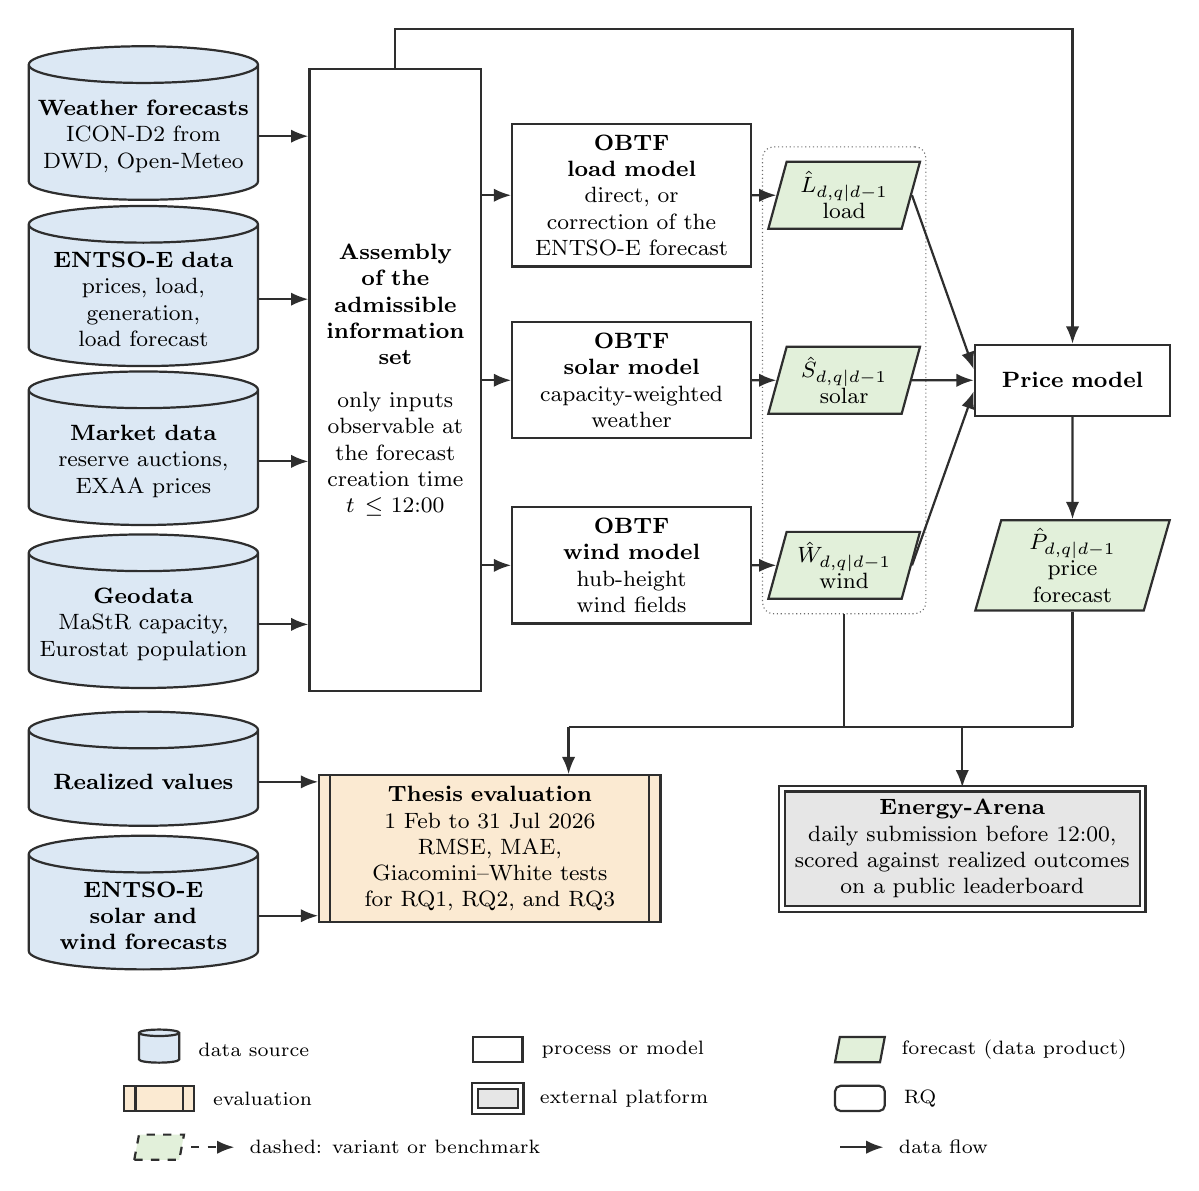
\begin{tikzpicture}[font=\footnotesize]

% ---------------- stage 1: data sources ----------------
\node[fgdata=2.7cm, minimum height=1.95cm] (wx)  at (0, 3.1)
  {\textbf{Weather forecasts}\\ICON-D2 from\\DWD, Open-Meteo};
\node[fgdata=2.7cm, minimum height=1.95cm] (ent) at (0, 1.03)
  {\textbf{\mbox{ENTSO-E} data}\\prices, load, generation,\\load forecast};
\node[fgdata=2.7cm, minimum height=1.95cm] (mkt) at (0,-1.03)
  {\textbf{Market data}\\reserve auctions,\\EXAA prices};
\node[fgdata=2.7cm, minimum height=1.95cm] (geo) at (0,-3.1)
  {\textbf{Geodata}\\MaStR capacity,\\Eurostat population};

% ---------------- stage 2: input assembly ----------------
\node[fgproc=1.9cm, minimum height=7.9cm] (asm) at (3.2, 0)
  {\textbf{Assembly of the admissible information set}\\[6pt]
   only inputs observable at the forecast creation time \(t \le\) 12:00};

% ---------------- stage 3: component models ----------------
\node[fgproc=2.75cm] (mload) at (6.2, 2.35)
  {\textbf{OBTF}\\\textbf{load model}\\direct, or correction of the \mbox{ENTSO-E} forecast};
\node[fgproc=2.75cm] (msol)  at (6.2, 0)
  {\textbf{OBTF}\\\textbf{solar model}\\capacity-weighted\\weather};
\node[fgproc=2.75cm] (mwind) at (6.2,-2.35)
  {\textbf{OBTF}\\\textbf{wind model}\\hub-height wind fields};

% ---------------- stage 4: component forecasts ----------------
\node[fgout=1.25cm] (fl) at (8.9, 2.35) {\(\hat{L}_{d,q|d-1}\)\\load};
\node[fgout=1.25cm] (fs) at (8.9, 0)    {\(\hat{S}_{d,q|d-1}\)\\solar};
\node[fgout=1.25cm] (fw) at (8.9,-2.35) {\(\hat{W}_{d,q|d-1}\)\\wind};
\begin{scope}[on background layer]
  \node[fggroup, fit=(fl)(fs)(fw)] (grp) {};
\end{scope}
% ---------------- stage 5: price model and forecast ----------------
\node[fgproc=2.2cm] (mprice) at (11.8, 0)
  {\textbf{Price model}};
\node[fgout=1.6cm] (fp) at (11.8,-2.35)
  {\(\hat{P}_{d,q|d-1}\)\\price forecast};

% ---------------- stage 6: evaluation and deployment ----------------
\node[fgdata=2.7cm, minimum height=1.45cm] (post) at (0,-5.1)
  {\textbf{Realized values}};
\node[fgdata=2.7cm, minimum height=1.45cm] (postent) at (0,-6.8)
  {\textbf{\mbox{ENTSO-E} solar and\\wind forecasts}};
\node[fgeval=3.7cm] (eval) at (4.4,-5.95)
  {\textbf{Thesis evaluation}\\1~Feb to 31~Jul~2026\\RMSE, MAE, Giacomini--White tests\\for RQ1, RQ2, and RQ3};
\node[fgext=4.3cm] (arena) at (10.4,-5.95)
  {\textbf{Energy-Arena}\\daily submission before 12:00,\\scored against realized outcomes\\on a public leaderboard};

% ---------------- flows ----------------
\foreach \s in {wx, ent, mkt, geo}
  \draw[fgflow] (\s.east) -- (\s.east -| asm.west);
\draw[fgflow] (asm.east |- mload) -- (mload.west);
\draw[fgflow] (asm.east |- msol)  -- (msol.west);
\draw[fgflow] (asm.east |- mwind) -- (mwind.west);
\draw[fgflow] (mload.east) -- (fl.west);
\draw[fgflow] (msol.east)  -- (fs.west);
\draw[fgflow] (mwind.east) -- (fw.west);
\draw[fgflow] (fl.east) -- ([yshift=4pt]mprice.west);
\draw[fgflow] (fs.east) -- (mprice.west);
\draw[fgflow] (fw.east) -- ([yshift=-4pt]mprice.west);
\draw[fgflow] (mprice.south) -- (fp.north);

% direct price-model inputs (top channel)
\draw[fgflow] (asm.north) -- ++(0,0.5) -| (mprice.north);

% forecasts to evaluation and benchmark (bus)
\coordinate (bus) at (0,-4.4);
\draw[thick, draw=fgLine] (grp.south) -- (grp.south |- bus);
\draw[thick, draw=fgLine] (fp.south)  -- (fp.south |- bus);
\draw[thick, draw=fgLine] (5.4,0 |- bus) -- (fp.south |- bus);
\draw[fgflow] (5.4,0 |- bus) -- (5.4,0 |- eval.north);
\draw[fgflow] (arena.north |- bus) -- (arena.north);
\draw[fgflow] (post.east) -- (post.east -| eval.west);
\draw[fgflow] (postent.east) -- (postent.east -| eval.west);

% ---------------- legend (two rows) ----------------
\begin{scope}[shift={(0.2,-8.5)}]
  \node[fgdata=0.3cm, minimum height=0.42cm] (k1) at (0,0) {};
  \node[right=3pt of k1, font=\scriptsize] {data source};
  \node[fgproc=0.35cm, minimum height=0.32cm] (k2) at (4.3,0) {};
  \node[right=3pt of k2, font=\scriptsize] {process or model};
  \node[fgout=0.3cm, minimum height=0.32cm] (k3) at (8.9,0) {};
  \node[right=3pt of k3, font=\scriptsize] {forecast (data product)};
  \node[fgeval=0.25cm, minimum height=0.32cm] (k4) at (0,-0.62) {};
  \node[right=3pt of k4, font=\scriptsize] {evaluation};
  \node[fgext=0.3cm, minimum height=0.32cm] (k5) at (4.3,-0.62) {};
  \node[right=3pt of k5, font=\scriptsize] {external platform};
  \node[fgrq=0.35cm, minimum height=0.32cm, rounded corners=2pt] (k6) at (8.9,-0.62) {};
  \node[right=3pt of k6, font=\scriptsize] {RQ};
  \node[fgout=0.3cm, minimum height=0.32cm, fgvar] (k7) at (0,-1.24) {};
  \draw[fgaux] ([xshift=3pt]k7.east) -- ++(0.55,0) coordinate (k7a);
  \node[right=2pt of k7a, font=\scriptsize] {dashed: variant or benchmark};
  \draw[fgflow] (8.65,-1.24) -- ++(0.55,0) coordinate (k8a);
  \node[right=2pt of k8a, font=\scriptsize] {data flow};
\end{scope}

\end{tikzpicture}%
}
\caption[Overview of the complete setup of the thesis.]
{Overview of the complete setup of the thesis, from the open data sources
through the forecasting models to the evaluation and the daily submission. The
legend applies to all process diagrams in this thesis.}
\label{fig:system_overview}
\end{figure}


In this setup, open data sources are assembled into the admissible information
set at the forecast creation time \(t\). This set feeds the OBTF load, solar, and wind models,
and the price model receives their forecasts together with further inputs from
the same set. All models are gradient-boosted trees. In RQ3, the pipeline is
rerun for each forecast creation time. The OBTF and price forecasts are
evaluated on the test period for RQ1 to RQ3. Data published only after gate
closure, namely the realized values and the \mbox{ENTSO-E} solar and wind
forecasts, are used only for evaluation and never as model inputs.

The pipeline is deployed operationally on the Energy-Arena platform
\cite{kleinebrahm2026energyarena}, which hosts separate forecasting challenges
for load, solar, wind, and the \mbox{DE-LU} day-ahead price, as
well as challenges tied to different forecast creation times. The pipeline
submits forecasts to each challenge every day before the corresponding
submission cutoff, which is the 12:00 gate closure for the day-ahead price
and correspondingly earlier for the challenges tied to earlier forecast
creation times. This deployment provides a live check that every model respects
the operational information cutoff and that the setup can be run end to end
under realistic timing constraints. The final configuration of each model in the
pipeline is summarized in Appendix~\ref{app:model_configs}.


\subsection{Problem Formulation}
\label{sec:problem_formulation}

This thesis considers the operational point forecasting problem of predicting
quarter-hourly day-ahead electricity prices in the \mbox{DE-LU} bidding zone. Let
\(P_{d,q}\) denote the realized day-ahead price for delivery
day \(d\) and market time unit (MTU) \(q\). On regular days, the day consists of
96 quarter-hourly MTUs, and the forecast for delivery day \(d\)
is created on day \(d-1\), the day before delivery. It must be available
before the day-ahead gate closure at
12:00 \cite{epexSpotPowerMarket}. For a forecast creation time
\(t\) on day \(d-1\), the price forecasting task is written as
\[
  \hat{P}_{d,q|d-1} = f(\mathcal{F}_{d-1}^{t}, q),
  \quad q \in \mathcal{Q}_d,
\]
where \(\hat{P}_{d,q|d-1}\) is the point forecast for delivery day \(d\),
\(\mathcal{Q}_d\) is the set of MTUs, and
\(\mathcal{F}_{d-1}^{t}\) is the information set available at time \(t\). Unless
stated otherwise, the information cutoff is set to the latest feasible
pre-gate-closure time, \(t=12{:}00\), and the forecast is computed and submitted
slightly before the 12:00 deadline.

The central idea is to generate forecasts of load, solar, and wind generation inside the same operational information set and then use them as
explicit inputs to the price model. The full notation is collected in the
List of Symbols. The OBTF forecasts are
\[
\begin{aligned}
  \hat{L}_{d,q|d-1} &= g^{\mathrm{load}}(\mathcal{F}_{d-1}^{t}, q), \\
  \hat{S}_{d,q|d-1} &= g^{\mathrm{solar}}(\mathcal{F}_{d-1}^{t}, q), \\
  \hat{W}_{d,q|d-1} &= g^{\mathrm{wind}}(\mathcal{F}_{d-1}^{t}, q).
\end{aligned}
\]
The OBTF solar and wind forecasts are combined into the OBTF renewable-generation
forecast
\[
  \hat{G}^{\mathrm{ren}}_{d,q|d-1}
  =
  \hat{S}_{d,q|d-1} + \hat{W}_{d,q|d-1},
\]
because the price responds to the total renewable feed-in that lowers residual
load rather than to the split between the two sources
(Section~\ref{sec:price_model}). Both are still forecast separately by their own
models.
Together with the OBTF load forecast, this defines the OBTF residual-load
forecast,
\[
  \widehat{RL}_{d,q|d-1}
  =
  \hat{L}_{d,q|d-1} - \hat{G}^{\mathrm{ren}}_{d,q|d-1}.
\]
The base price forecast, without the OBTF load, renewable-generation, and
residual-load forecasts, is denoted
\(\hat{P}^{\mathrm{base}}_{d,q|d-1}\). The price forecast with OBTF load and renewable-generation inputs, namely \(\hat{L}_{d,q|d-1}\),
\(\hat{G}^{\mathrm{ren}}_{d,q|d-1}\), and
\(\widehat{RL}_{d,q|d-1}\), is denoted
\(\hat{P}^{\mathrm{gen}}_{d,q|d-1}\). These objects define the comparisons
examined in the experimental design
(Section~\ref{sec:experimental_design}).

\subsection{Data}
\label{sec:data}

\subsubsection{Target Variable and Temporal Scope}
\label{sec:target_temporal_scope}

The target variable is the realized \mbox{DE-LU} day-ahead auction price \(P_{d,q}\),
measured in EUR/MWh. The German day-ahead market changed from hourly to
quarter-hourly market clearing on 1~October~2025
\cite{epexSpot15MinuteMarketCoupling}. Post-transition observations therefore
contain genuine 15-minute price variation, whereas pre-transition prices only
reflect hourly market clearing and are treated as historical proxy information
if they are used to extend a rolling training window. In that case, each hourly
price is expressed at quarter-hourly resolution by applying it to the four
quarter-hours of that hour, since pre-transition clearing set a single price for
the whole hour.

For model development and evaluation, the post-transition sample is split into
a development period and a held-out out-of-sample test period. The split, the
rolling estimation scheme, and their justification are defined in
Section~\ref{sec:experimental_design}.

All timestamped data are represented in the local market timezone
Europe/Berlin. To keep the model target dimension constant across delivery
days, daylight-saving transition days are mapped to the fixed 96-column
MTU representation used by the models: repeated autumn intervals
are averaged into their MTU, while missing spring intervals are
filled by within-day linear interpolation. The models and the reported evaluation use this fixed 96-unit representation, so
predicted and realized prices are always compared on the same grid. An
operational submission to Energy-Arena, which scores each delivery
day on its actual MTU grid of 92, 96, or 100 units on 23-, 24-, and
25-hour days, maps the 96-unit forecast back to those units on the two transition
days, dropping the interpolated spring units and expanding the averaged autumn
units to their two occurrences.

Figure~\ref{fig:target_price_characteristics} summarizes the empirical
behavior of the post-transition target series in the available descriptive
sample from 1~October~2025 to 31~July~2026. Prices are volatile and
asymmetric, with realized values ranging from -499.99 to 747.10~EUR/MWh and
5.8\% of observed MTUs taking negative values. The average
intraday profile shows lower prices around midday and higher prices during
morning and evening demand periods, which motivates the use of price lags,
calendar variables, weather information, load, and renewable generation.

\begin{figure}[htbp]
  \centering
  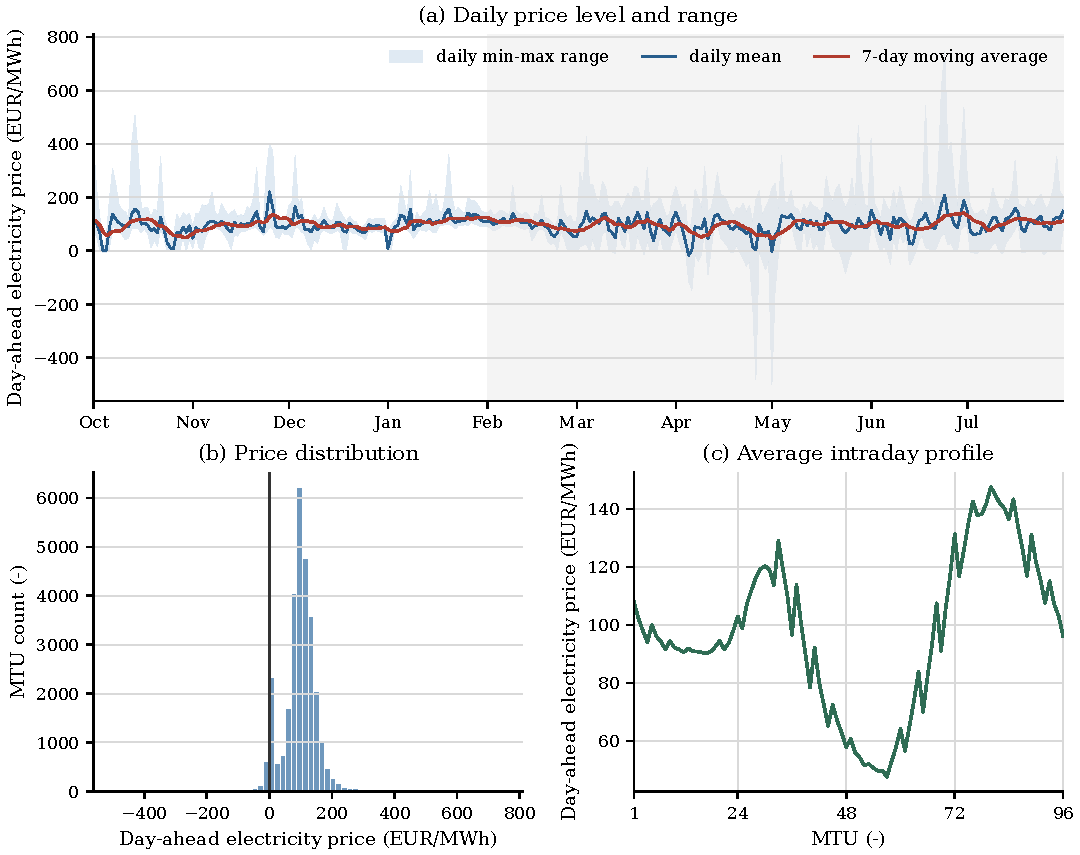
\includegraphics[width=\textwidth]{figures/target_price_characteristics.pdf}
  \caption[Empirical characteristics of the \mbox{DE-LU} day-ahead price target.]
  {Empirical characteristics of the \mbox{DE-LU} day-ahead price target in the
  available post-transition sample from 1~October~2025 to 31~July~2026. The top
  panel shows daily mean prices together with the daily minimum-maximum range
  and a seven-day moving average. The shaded area marks the fixed
  out-of-sample test period from 1~February~2026 to 31~July~2026. The lower
  panels show the empirical price distribution and the average intraday price
  profile across MTUs.}
  \label{fig:target_price_characteristics}
\end{figure}

\subsubsection{Input Data Sources and Derived Covariates}
\label{sec:input_data_sources}

The market-price data consist of realized \mbox{DE-LU} Single Day-Ahead Coupling (SDAC)
auction prices from the \mbox{ENTSO-E} Transparency Platform
\cite{entsoeTransparency}. They define the price target and provide lagged
price features that capture short-term dependence and recurring price patterns
in electricity price forecasting \cite{weron2014electricity,lago2021forecasting}.
Prices from the Energy Exchange Austria (EXAA) are treated as an
optional late market signal, because prices from this earlier auction carry
predictive information for other European day-ahead markets
\cite{ziel2015exaa}. The EXAA auction closes at 10:15
\cite{exaaTradingRules2025}, and the resulting \mbox{DE-LU} day-ahead prices are
published on the \mbox{ENTSO-E} Transparency Platform around 11:15
\cite{entsoeTransparency,eiser2026operational}.
Neighboring SDAC prices are excluded because they are released only after the
12:00 gate closure \cite{epexSpotPowerMarket}.

For the cutoff experiment, the price model also uses German control-reserve
auction results from Regelleistung.net at every cutoff after their publication
\cite{regelleistungNet2026}. Control reserve is the
balancing capacity that transmission system operators (TSOs) procure ahead of delivery
to keep grid frequency stable, split by activation speed into frequency
containment reserve (FCR), automatic frequency restoration reserve (aFRR), and manual
frequency restoration reserve (mFRR), and cleared in daily capacity auctions on the day
before delivery. The covariates summarize the published outcomes of these
auctions. They are included because capacity committed to control reserve is
withheld from the energy market and reserve prices reflect the expected scarcity
of flexible capacity. The auction outcomes are therefore expected to carry an
early signal of system tightness, which in a fundamental view shapes the
day-ahead price through the conventional supply stack \cite{pape2016fundamentals}. Together with the EXAA price signal,
these reserve-market covariates are early market signals rather than explicit
load or renewable-generation representations, so they are held out of \hyperlink{rq:component_forecast_quality}{RQ1}
and \hyperlink{rq:price_impact_generated_forecasts}{RQ2}, which study the
OBTF load and renewable-generation forecasts and their price impact without early market
information. They enter only in
\hyperlink{rq:cutoff_sensitivity}{RQ3}, where their staggered availability
across the morning is part of the information-accrual design.

Load and renewable-generation data are also obtained from \mbox{ENTSO-E}
\cite{entsoeTransparency}. For load, the pipeline uses lagged actual load,
morning actual load observed before the forecast creation time, and the public
day-ahead load forecast once it has been published before gate closure. For
renewables, realized solar generation and realized onshore and offshore wind
generation define the targets for the solar and wind forecasting models. The
\mbox{ENTSO-E} day-ahead solar and wind generation forecasts serve as
benchmarks for \hyperlink{rq:component_forecast_quality}{RQ1} but not
as price model inputs, because they are not publicly observable before gate
closure. The
publication times of all inputs and their regulatory basis are documented in
Section~\ref{sec:operational_information_set}. Load, solar, and wind are
economically relevant because demand and renewable feed-in shift the
short-run supply-demand balance and thus the merit order
\cite{sensfuss2008meritOrder}.

Weather forecasts provide the main exogenous inputs for the OBTF forecasts of
load, solar, and wind generation. The primary weather model is
\mbox{ICON-D2}, the high-resolution short-range configuration of ICON that the DWD
runs for Germany and its neighboring regions. Its forecasts are obtained both from
DWD Open Data and through the Open-Meteo API
\cite{zaengl2015icon,dwdIconForecastData,openMeteoForecastApi}. A new run starts
every three hours. Each run is named after its start time in Coordinated Universal Time (UTC), so the 06~UTC run
starts at 08:00 local summer time. A run is complete about 80~minutes after its
start, which makes the 06~UTC run available at about 09:20 local time in summer
and one hour earlier in winter. All models rely on this single weather model. The OBTF wind model additionally uses its hub-height wind
fields from Open-Meteo, described in Section~\ref{sec:wind_model}. The weather variables include
temperature, humidity, wind conditions, solar radiation, cloud cover,
precipitation, snow, and atmospheric pressure. These variables are physically
linked to load through heating and cooling demand
\cite{hong2016probabilisticLoad}, to photovoltaic generation through radiation
and cloud cover \cite{antonanzas2016pvForecasting}, and to wind generation
through wind speed and wind direction
\cite{foley2012windForecasting}. Installed renewable capacity from the
MaStR connects the weather fields to the generation fleet
\cite{bundesnetzagenturMastr}, and gridded population data from Eurostat
connect the weather fields to the demand side for load-oriented aggregation
\cite{eurostatGisco2021}. Calendar covariates comprise weekday indicators and a
German public-holiday flag taken from public-holiday calendars
\cite{pythonHolidays}.

\subsection{Operational Information Set}
\label{sec:operational_information_set}

All model inputs are restricted to information that would have been available
at the forecast creation time. For a local forecast creation time \(t\) on day
\(d-1\), the admissible information set is
\[
  \mathcal{F}_{d-1}^{t}
  =
  \left\{
    Z_{s} \mid \operatorname{avail}(Z_{s})
    \leq \tau_{d-1}^{t}
  \right\},
\]
where \(Z_{s}\) is an observation, forecast, or derived feature with reference
time \(s\), \(\operatorname{avail}(Z_{s})\) is the time at which it becomes
available to the pipeline, and \(\tau_{d-1}^{t}\) is the clock time \(t\) on day
\(d-1\). This rule is a
leakage constraint. It does not imply that every model uses every available
input.

In \hyperlink{rq:component_forecast_quality}{RQ1} and
\hyperlink{rq:price_impact_generated_forecasts}{RQ2}, forecasts are created with the
latest feasible pre-gate-closure information set
\(\mathcal{F}_{d-1}^{12:00}\), with computation and submission completed
slightly before 12:00. \hyperlink{rq:cutoff_sensitivity}{RQ3}
varies the forecast creation time over the following times on day
\(d-1\):
\[
  \mathcal{T}^{\mathrm{cut}}
  =
  \{07{:}00,08{:}00,09{:}00,10{:}00,11{:}00,12{:}00\}.
\]
At each cutoff, every input block enters only once it is published, and the
derived forecasts are rebuilt from the cutoff-specific information set.
Figure~\ref{fig:operational_timeline} summarizes the timing of the main data
blocks, Table~\ref{tab:cutoff_accrual} lists the inputs available at each
cutoff, and Appendix~\ref{app:data_timing} documents the sources behind the
availability assumptions.

The availability constraint abstracts from computation time, treating \(t\) as a
pure information cutoff and assuming the forecast is produced before gate
closure. In a strict operational sense the admissible cutoff is earlier than
\(t\) by the pipeline runtime, so a later cutoff, or a more expensive model,
trades computation time for information. In the live deployment, the creation
times \(t\) are the submission deadlines of the corresponding Energy-Arena
challenges \cite{kleinebrahm2026energyarena}. Each model run starts 20~minutes
before its deadline and submits before it, so the operational information cutoff
lies up to 20~minutes before \(t\). Because the pipeline relies on lightweight
boosted-tree models, this budget is short relative to the one-hour spacing of the
cutoff grid, and the cutoff experiment isolates the value of information rather
than a computation-time budget.

\begin{figure}[htbp]
\centering
\resizebox{0.97\textwidth}{!}{%
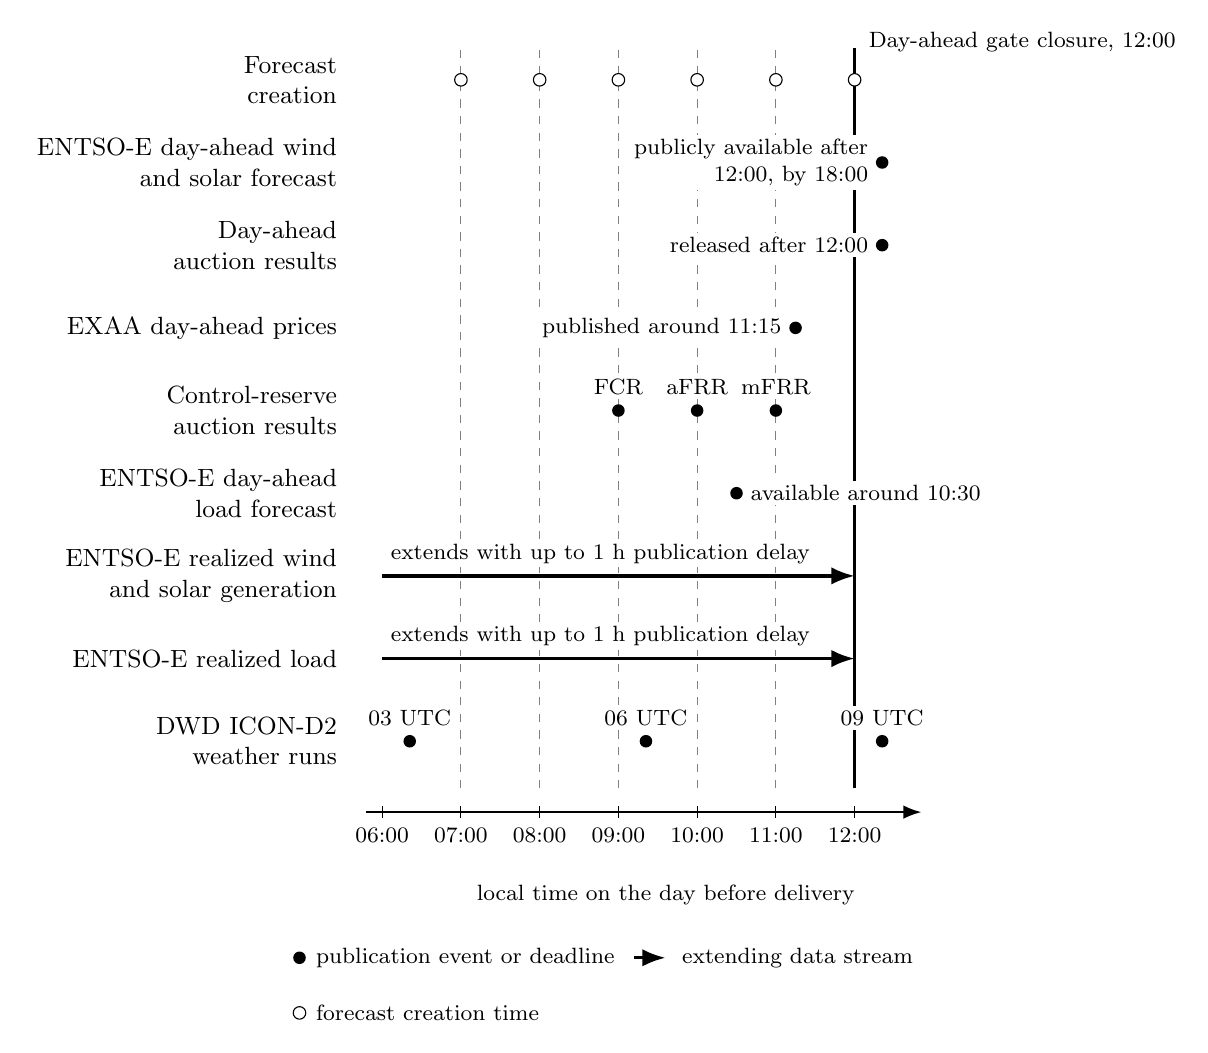
\begin{tikzpicture}[
    >=Latex,
    font=\small,
    rowlabel/.style={anchor=east, align=right, font=\small},
    event/.style={circle, fill=black, inner sep=1.6pt},
    gen/.style={circle, draw=black, fill=white, inner sep=1.6pt},
    note/.style={font=\footnotesize, inner sep=1.5pt, fill=white},
    stream/.style={very thick},
    cutoff/.style={dashed, gray}
]

% time-to-x mapping: x = t - 6, local clock time t on day d-1

% ---- cutoff grid and gate closure ----
\foreach \t in {7, 8, 9, 10, 11} {
  \draw[cutoff] ({\t-6},0.3) -- ({\t-6},9.7);
}
\draw[very thick] (6.0,0.3) -- (6.0,9.7);
\node[note, anchor=south west] at (6.12,9.6) {Day-ahead gate closure, 12:00};

% ---- time axis ----
\draw[->, thick] (-0.2,0) -- (6.85,0);
\foreach \t/\l in {6/06:00, 7/07:00, 8/08:00, 9/09:00, 10/10:00, 11/11:00,
                   12/12:00} {
  \draw ({\t-6},0.08) -- ({\t-6},-0.08)
    node[below, font=\footnotesize] {\l};
}
\node[font=\footnotesize] at (3.6,-1.05)
  {local time on the day before delivery};

% ---- data rows ----
\node[rowlabel] at (-0.45,0.9) {DWD ICON-D2\\weather runs};
\node[event] at (0.35,0.9) {};
\node[note, anchor=south] at (0.35,1.04) {03 UTC};
\node[event] at (3.35,0.9) {};
\node[note, anchor=south] at (3.35,1.04) {06 UTC};
\node[event] at (6.35,0.9) {};
\node[note, anchor=south] at (6.35,1.04) {09 UTC};

\node[rowlabel] at (-0.45,1.95) {ENTSO-E realized load};
\draw[stream,->] (0,1.95) -- (6.0,1.95);
\node[note, anchor=south west] at (0.05,2.05)
  {extends with up to 1 h publication delay};

\node[rowlabel] at (-0.45,3.0) {ENTSO-E realized wind\\and solar generation};
\draw[stream,->] (0,3.0) -- (6.0,3.0);
\node[note, anchor=south west] at (0.05,3.1)
  {extends with up to 1 h publication delay};

\node[rowlabel] at (-0.45,4.05) {ENTSO-E day-ahead\\load forecast};
\node[event] at (4.5,4.05) {};
\node[note, anchor=west] at (4.62,4.05) {available around 10:30};

\node[rowlabel] at (-0.45,5.1) {Control-reserve\\auction results};
\node[event] at (3.0,5.1) {};
\node[note, anchor=south] at (3.0,5.24) {FCR};
\node[event] at (4.0,5.1) {};
\node[note, anchor=south] at (4.0,5.24) {aFRR};
\node[event] at (5.0,5.1) {};
\node[note, anchor=south] at (5.0,5.24) {mFRR};

\node[rowlabel] at (-0.45,6.15) {EXAA day-ahead prices};
\node[event] at (5.25,6.15) {};
\node[note, anchor=east] at (5.13,6.15) {published around 11:15};

\node[rowlabel] at (-0.45,7.2) {Day-ahead\\auction results};
\node[event] at (6.35,7.2) {};
\node[note, anchor=east] at (6.23,7.2) {released after 12:00};

\node[rowlabel] at (-0.45,8.25) {ENTSO-E day-ahead wind\\and solar forecast};
\node[event] at (6.35,8.25) {};
\node[note, anchor=east, align=right] at (6.23,8.25)
  {publicly available after\\12:00, by 18:00};

% ---- model-run row ----
\node[rowlabel] at (-0.45,9.3) {Forecast\\creation};
\foreach \t in {7, 8, 9, 10, 11, 12} {
  \node[gen] at ({\t-6},9.3) {};
}

% ---- legend ----
\node[event] at (-1.05,-1.85) {};
\node[note, anchor=west] at (-0.9,-1.85) {publication event or deadline};
\draw[stream,->] (3.2,-1.85) -- (3.6,-1.85);
\node[note, anchor=west] at (3.75,-1.85) {extending data stream};
\node[gen] at (-1.05,-2.55) {};
\node[note, anchor=west, align=left] at (-0.9,-2.55)
  {forecast creation time};

\end{tikzpicture}%
}
\caption[Operational overview of data availability and forecast creation
times on the day before delivery.]
{Operational overview of data availability, forecast creation times, and
model runs on the day before delivery
\cite{euRegulation543_2013,kleinebrahm2026energyarena,exaaTradingRules2025,dwdIconForecastData,openMeteoForecastApi}.
The dashed grid marks the forecast creation times in local time.
Times are shown for summer time. Events to the right of 12:00 are not drawn to
scale.}
\label{fig:operational_timeline}
\end{figure}


\subsection{Forecasting Models}
\label{sec:component_forecast_models}

All learned forecasting tasks in this thesis use gradient-boosted regression
trees \cite{friedman2001gbm}. The same model family is used for load, solar,
wind, and price forecasting, which keeps the methodology consistent across
tasks. Gradient-boosted trees are well suited to the heterogeneous tabular
feature sets used here, on which they remain a strong and frequently superior
alternative to deep-learning models
\cite{grinsztajn2022tree,shwartzziv2022tabular}.
Boosted trees handle nonlinear relationships and interactions between
weather, calendar, lagged values, and market variables without requiring these
interactions to be specified manually
\cite{hastie2009elements,friedman2001gbm}. The implementation uses
efficient histogram-based boosted-tree regressors from scikit-learn and
LightGBM \cite{pedregosa2011sklearn,ke2017lightgbm}. Because both estimators
belong to the same model family, the estimator choice is treated as an
implementation detail and not as a separate research comparison.

\subsubsection{Weather Representations}
\label{sec:weather_representations}

All models use the DWD \mbox{ICON-D2} forecast as their weather input
(Section~\ref{sec:data}). \mbox{ICON-D2} is a gridded numerical weather
prediction that reports several weather variables at many grid points across
the bidding zone, mostly
at hourly resolution and for solar radiation at quarter-hourly resolution. Used
directly, the
number of raw grid features would far exceed the at most a few hundred daily
training observations in the rolling training window, a regime in which boosted
trees tend to overfit noise rather than learn the weather-to-target relationship. Because neighboring grid
points are strongly correlated, most of this dimensionality is redundant. Each
field is therefore converted into a fixed set of model features before it enters
the load, solar, wind, and price models: the grid points are grouped into a
small number of spatial clusters of nearby locations, and each cluster is
summarized by a weighted spatial average of every weather variable. This limits
the feature count and the resulting overfitting while retaining the weather
signal relevant for price and generation.
Clustering is preferred to a generic projection such as principal components
\cite{hastie2009elements} because it preserves the physical and spatial meaning of each feature and,
unlike orthogonal components, lets the aggregation be weighted by where the
target actually forms: population where demand matters and installed capacity
where generation matters. Spatial aggregation of gridded weather into
lower-dimensional features is also established practice in comparable
operational forecasting pipelines \cite{eiser2026operational}.
For the OBTF load, solar, and wind models, the thesis does not study alternative
clustering designs in a separate RQ, but describes the final spatial
representations used in the pipeline.
For the raw weather variables used directly by the price model, the spatial
representation is instead selected on the development period, so that the comparison of the RQ2 base forecast
\(\hat{P}^{\mathrm{base}}_{d,q|d-1}\) with the forecasts using OBTF inputs isolates
the effect of the OBTF forecasts rather than that of a suboptimal weather
aggregation. Starting from the five-cluster aggregation of
the operational price forecasting pipeline of \textcite{eiser2026operational}, the
number of clusters is varied and the development-period forecast error is
minimized, which yields a two-cluster aggregation. Finer spatial resolutions do
not improve development-period accuracy and raise the daily training cost
steeply, as reported in Appendix~\ref{app:price_results}. This selection remains
a baseline design choice rather than a separate RQ.

For load, weather variables are summarized into \mbox{DE-LU}-level features on a
25-cluster weather grid. The spatial means are population-weighted, because
demand depends on the weather experienced by consumers.
Since load is concentrated where people live, an unweighted spatial mean would
over-represent sparsely populated areas that contribute little demand, whereas a
population-weighted mean better reflects the weather in the densely populated
areas that drive most demand.
Population-weighted temperature and the derived degree-day variables are
long-established predictors in load forecasting
\cite{hong2016probabilisticLoad}. The weighting is applied explicitly rather
than left for the model to learn implicitly, because estimating the per-cluster
weights from a short rolling training window would be data-inefficient and prone
to overfitting, whereas the population--demand link is a reliable prior grounded
in the load-forecasting literature. For
solar generation, weather features are aligned with the distribution of
installed photovoltaic capacity from the MaStR, using 25
clusters per TSO proxy area. A proxy area
approximates a control area by the federal states it mainly covers, and
installed capacity is assigned to it through the federal state recorded in the
MaStR. For wind
generation, weather features are aligned with installed wind capacity through a
100-cluster representation that includes offshore sites. This keeps
the physical link between weather and the corresponding target. The cluster
counts are chosen on the development period to balance the bias-variance
trade-off rather than studied in a separate RQ: coarser grids
oversmooth the field and underfit the capacity or demand distribution, while
finer grids add correlated, redundant features that the data-limited models
overfit. Solar and wind use finer grids than load because generation is
concentrated at specific sites and spatially heterogeneous, whereas demand is
smooth and is represented at the coarser \mbox{DE-LU} level. Wind in particular
responds to local wind speed through a nonlinear power curve
\cite{bandi2016powerCurve} and is concentrated at specific onshore and offshore
sites. The resulting
spatial representations are illustrated in
Figure~\ref{fig:spatial_weather_representations}.

\begin{figure}[htbp]
  \centering
  \begin{subfigure}{0.32\textwidth}
    \centering
    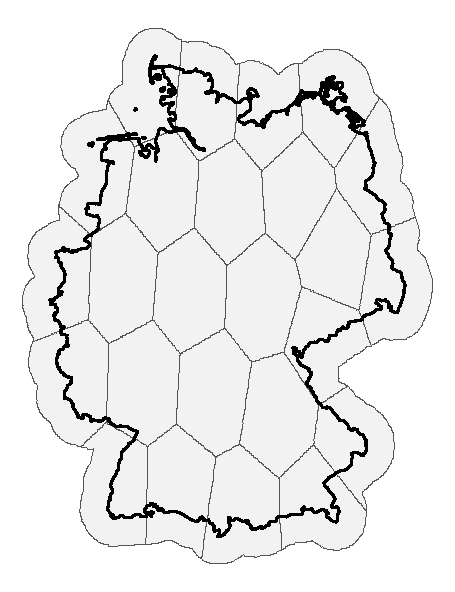
\includegraphics[width=\linewidth]{figures/spatial_weather_load_clusters.pdf}
    \caption{Load}
  \end{subfigure}
  \hfill
  \begin{subfigure}{0.33\textwidth}
    \centering
    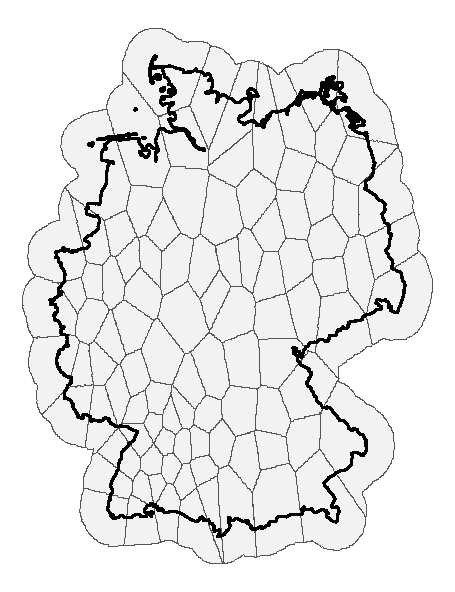
\includegraphics[width=\linewidth]{figures/spatial_weather_solar_clusters.pdf}
    \caption{Solar generation}
  \end{subfigure}
  \hfill
  \begin{subfigure}{0.32\textwidth}
    \centering
    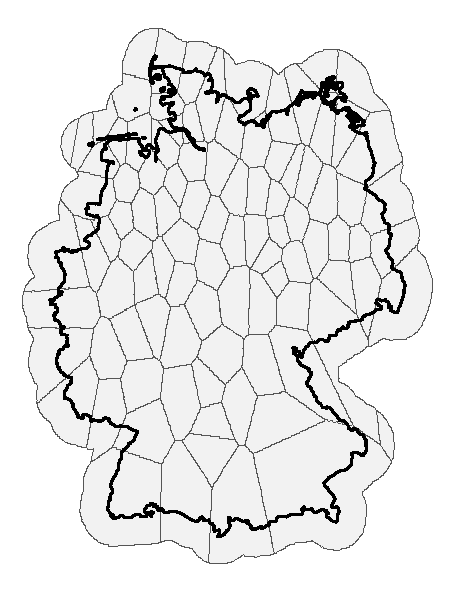
\includegraphics[width=\linewidth]{figures/spatial_weather_wind_clusters.pdf}
    \caption{Wind generation}
  \end{subfigure}
  \caption[Spatial weather representations of the forecasting models.]
  {Spatial weather representations of the forecasting models. Panel~(a) shows
  the 25-cluster weather grid used to construct population-weighted
  load-weather features. Panel~(b) shows the solar representation with 25
  clusters per TSO proxy area. Panel~(c) shows the 100-cluster wind
  representation including offshore sites.}
  \label{fig:spatial_weather_representations}
\end{figure}

\FloatBarrier

\subsubsection{OBTF Load Model}
\label{sec:load_model}

The OBTF load model predicts realized \mbox{DE-LU} load \(L_{d,q}\) for delivery day \(d\)
and MTU \(q\), producing a complete 96-MTU load curve for the
delivery day. The resulting OBTF load forecast is denoted \(\hat{L}_{d,q|d-1}\). The
model is re-estimated in a rolling scheme with a boosted-tree regressor and
uses calendar and holiday variables, lagged realized load, actual load
observed during the morning before forecast creation, weather features, and,
when available, the public \mbox{ENTSO-E} load forecast. For training, realized
load of day \(d-1\) is used only up to the last quarter-hour published before
forecast creation.

The weather block starts from cluster-level forecasts of temperature, dew
point, surface pressure, precipitation, snow depth, cloud cover, solar
radiation, and wind speed. From temperature and dew point, the pipeline derives
relative humidity, vapor-pressure deficit, and heating and cooling degree
variables. Rather than using the 25 cluster series individually, the OBTF load model summarizes
them into a compact set of \mbox{DE-LU}-wide features.
Population-weighted means describe the average weather exposure of consumers,
while daily summaries capture the mean, minimum, maximum, and range of selected
weather variables over the delivery day. Spatial weather quantiles describe the
distribution across clusters at a given MTU, for example the lower, median, and
upper part of the temperature or cloud-cover distribution. They are
descriptive spatial quantiles, not probabilistic forecast quantiles, and are
complemented by cross-cluster spread measures such as ranges and standard
deviations. These features describe whether a weather extreme is confined to one part of the
zone or spread across all of it, which affects aggregate demand beyond what the
population-weighted mean captures.

The model has two operational modes. Before the public load forecast becomes
available, it predicts load directly from the admissible input data. Once the
public load forecast is available, the final model uses a forecast-correction
specification. Let \(L^{\mathrm{ENTSOE}}_{d,q|d-1}\) denote the public
\mbox{ENTSO-E} load forecast, with the correction target defined as the
forecast deviation
\[
  \Delta^{L}_{d,q}
  =
  L_{d,q} - L^{\mathrm{ENTSOE}}_{d,q|d-1},
\]
and adds the predicted correction back to the public forecast,
\[
  \hat{L}_{d,q|d-1}
  =
  L^{\mathrm{ENTSOE}}_{d,q|d-1} + \hat{\Delta}^{L}_{d,q|d-1}.
\]
This treats the \mbox{ENTSO-E} forecast as an admissible baseline and uses the
model to correct remaining errors with the available load, calendar, and
weather information. The public forecast is produced by the system operators
with undisclosed models and inputs \cite{euRegulation543_2013,entsoeTransparency},
which cannot be reconstructed from the open data available here. Correcting it
lets the model add whatever information the public forecast does not already
reflect, namely its systematic errors, information that arrived after it was
issued, such as newer weather runs and the morning's realized load, and
information that was available but is not exploited by the undisclosed model. Predicting this correction rather than the
load level is also favorable in bias-variance terms: the correction is a small
and comparatively stationary target with far less variance than the full load
curve, so a model trained on only a few hundred rolling days estimates it more
reliably than it could estimate load from scratch. The direct mode is relevant for early forecast
creation times in RQ3, while the correction mode is used whenever the public
load forecast is available.

\subsubsection{OBTF Solar Model}
\label{sec:solar_model}

The OBTF solar model predicts realized solar generation \(S_{d,q}\) for all 96
MTUs of the delivery day. The resulting OBTF solar forecast is denoted
\(\hat{S}_{d,q|d-1}\). In the empirical analysis, the model is implemented
with histogram-based boosted trees and estimated on a rolling training window.
It is trained separately for the four German control areas of 50Hertz,
Amprion, TenneT, and TransnetBW, because realized solar generation is published
per control area and the bidding-zone value is essentially their sum. In the
test period, the four areas account for 99.4\% of realized \mbox{DE-LU} solar
generation, with the remainder from Luxembourg. Summing the four area forecasts
to the aggregate OBTF solar forecast therefore mirrors how the realized
value is composed.

The inputs are calendar variables, installed photovoltaic capacity, the position
of the sun, and weather. Realized generation is not used as a lagged input. It
enters only as the training target and through the bias correction described
below. The weather is aggregated over 25 clusters per TSO proxy area
(Section~\ref{sec:weather_representations}) and weighted by installed
photovoltaic capacity. It includes irradiance, temperature,
precipitation, snow, and cloud cover, together with spread measures that
distinguish uniformly cloudy areas from areas where conditions differ across
locations.

The model also uses a physics-based solar baseline, the expected photovoltaic
generation computed from the forecast irradiance and temperature, the position
of the sun, and the installed capacity \cite{antonanzas2016pvForecasting}. The
boosted-tree model then predicts only the deviation from this baseline, which
keeps the forecast physically plausible. Training days on which realized
generation falls far below the baseline under clear-sky conditions, a pattern
more consistent with data errors or curtailment than with weather, are
excluded. Predictions are finally adjusted with a rolling bias correction that
subtracts the average error of recent days, applied per control area and to the
\mbox{DE-LU} total, which also covers the small Luxembourg share.

\subsubsection{OBTF Wind Model}
\label{sec:wind_model}

The OBTF wind model predicts realized wind generation \(W_{d,q}\), including both
onshore and offshore generation, for all 96 MTUs of the delivery day. The
resulting OBTF wind forecast is denoted \(\hat{W}_{d,q|d-1}\). In the
empirical analysis, the model is implemented with histogram-based boosted
trees and estimated on a rolling training window. Onshore and offshore
generation are forecast separately, because they differ in their weather drivers
and spatial concentration and are published as separate production types
\cite{entsoeTransparency}. The two forecasts are then summed to the aggregate
OBTF wind forecast used by the price model.

The inputs are calendar variables, installed wind capacity, and weather. As for
solar, realized generation enters only as the training target and through the
bias correction. The weather is aggregated over 100 clusters including offshore
sites (Section~\ref{sec:weather_representations}), grouped into an offshore
region and five onshore regions, and weighted by installed wind capacity. It
includes wind speed and direction, temperature, and precipitation. Because wind
generation rises nonlinearly with wind speed, the model also uses transformed
wind speeds that approximate a turbine power curve \cite{bandi2016powerCurve}.
From the same \mbox{ICON-D2} run, accessed through Open-Meteo
\cite{openMeteoForecastApi}, it additionally uses wind speeds at typical turbine
hub heights between 80 and 180~m, because generation is especially sensitive to
the wind at hub height \cite{bandi2016powerCurve,foley2012windForecasting}. Predictions are corrected with the same rolling bias
correction as for solar.

\subsubsection{Price Model}
\label{sec:price_model}
\label{sec:price_features}

The price model predicts \(P_{d,q}\) with boosted trees. Before fitting, the
price target is robustly standardized and passed through an inverse hyperbolic
sine transform \cite{uniejewski2018variance}, which stabilizes the variance of
the volatile, spike-prone, and occasionally negative price series, and
predictions are transformed back to price levels for evaluation. As is common in
day-ahead price forecasting, a separate model is fitted for each MTU, because the price level and its drivers differ strongly across the day
\cite{lago2021forecasting}. In RQ2, the base
price forecast \(\hat{P}^{\mathrm{base}}_{d,q|d-1}\) is compared with the
price forecast with OBTF load and renewable-generation forecasts
\(\hat{P}^{\mathrm{gen}}_{d,q|d-1}\). The base price forecast uses price lags,
calendar variables, weather variables, and the published \mbox{ENTSO-E}
day-ahead load forecast, and excludes early cross-market
price signals. The price forecast with OBTF load and renewable-generation forecasts uses the same
variables but replaces the \mbox{ENTSO-E} load forecast with the OBTF
load forecast \(\hat{L}_{d,q|d-1}\) and adds the OBTF combined
renewable-generation forecast \(\hat{G}^{\mathrm{ren}}_{d,q|d-1}\) and the
OBTF residual-load forecast \(\widehat{RL}_{d,q|d-1}\). Because these inputs are themselves model forecasts
rather than realized values, they enter the price model as forecasted inputs
and carry their own forecast error \cite{pagan1984generated}.
Solar and wind enter the price model as a single combined forecast rather than as
two separate inputs, because price formation responds to the total renewable
feed-in that lowers residual load rather than to the split between the two
sources, and a single input keeps the data-limited price model parsimonious. Both
are still forecast separately by their own models.
Residual load denotes load net of renewable generation and is also referred to
as residual demand or net load in the literature
\cite{do2021residualDemand}. It is included as an explicit input in addition
to load and combined renewable generation because it directly represents the
demand that must be met by dispatchable plants, which is the quantity that
sets the marginal price in the merit order \cite{sensfuss2008meritOrder}.
Providing residual load explicitly allows a single tree split to represent
this supply-demand balance, which the boosted-tree model would otherwise have
to recover from load and renewable generation through feature interactions.
This comparison isolates the value of \(\hat{L}_{d,q|d-1}\),
\(\hat{G}^{\mathrm{ren}}_{d,q|d-1}\), and
\(\widehat{RL}_{d,q|d-1}\) because the remaining price lags, calendar
variables, and weather variables are kept the same.
A weather-free price forecast with OBTF load and renewable-generation forecasts,
\(\hat{P}^{\mathrm{gen},-\mathrm{wea}}_{d,q|d-1}\), keeps these forecasts but omits the raw weather features. Because OBTF forecasts are themselves derived from weather, this variant tests
whether they provide a representation of the weather-driven system state that
can substitute for the raw weather inputs.
The cluster-level weather representations are not passed on to the price
model, but are used only inside the OBTF models. These models
first generate final forecasts for load, solar, and wind generation
for each MTU, and the price model receives only the three \mbox{DE-LU} totals
\(\hat{L}_{d,q|d-1}\), \(\hat{G}^{\mathrm{ren}}_{d,q|d-1}\), and
\(\widehat{RL}_{d,q|d-1}\). Intermediate outputs of the OBTF models, such as the separate OBTF solar and wind forecasts before they are combined or any
regional and cluster-level series, are not passed on.
The RQ3 timing experiment then changes the admissible input set according to
the forecast creation time. Additional inputs enter only after their
publication. In particular, reserve-market covariates are included only after
the corresponding Regelleistung.net auction-result blocks are available, and
EXAA prices enter only at the 12:00 cutoff.

Two design choices of the price model are fixed on the development period before
the test period is used. The raw weather variables used by the price model are aggregated to
two spatial clusters, as described in Section~\ref{sec:weather_representations},
and the rolling training window is set to 70 days, the shortest length beyond
which development-period accuracy no longer improves. The window is short
because price relationships shift quickly with fuel prices, renewable capacity,
and season, so recent days are more informative than older ones. These choices
are made with
the same boosted-tree setup for \(\hat{P}^{\mathrm{base}}_{d,q|d-1}\) and
\(\hat{P}^{\mathrm{gen}}_{d,q|d-1}\), so that the RQ2 comparison is not confounded
by a weaker base price forecast.
Appendix~\ref{app:price_results} reports both selection sweeps, including the
steep growth of the daily training cost with the number of weather clusters.

Two simple benchmark forecasts for the price forecast are included in
RQ2. The previous-day naive benchmark uses the realized price curve of delivery
day \(d-1\) as the forecast for day \(d\). The previous-week naive benchmark
uses the realized price curve of delivery day \(d-7\). Both benchmarks are
admissible before the 12:00 gate closure and provide an easily
interpretable baseline for the model-based price forecasts.
Table~\ref{tab:price_model_variants} summarizes the price forecast variants used
in RQ2 and RQ3.

\begin{table}[H]
  \centering
  \small
  \caption[Price forecast model variants and their inputs.]
  {Price forecast variants used in RQ2 and RQ3.}
  \label{tab:price_model_variants}
  \begin{tabular}{@{}>{\raggedright\arraybackslash}p{0.20\textwidth}
                  >{\raggedright\arraybackslash}p{0.70\textwidth}@{}}
    \toprule
    Variant & Description \\
    \midrule
    \(\mathrm{N}_{d-1}\)
    & Previous-day naive price forecast using the realized price curve of
      delivery day \(d-1\). \\
    \addlinespace
    \(\mathrm{N}_{d-7}\)
    & Previous-week naive price forecast using the realized price curve of
      delivery day \(d-7\). \\
    \addlinespace
    \(\hat{P}^{\mathrm{base}}_{d,q|d-1}\)
    & Base price forecast from the boosted-tree model using the
      \mbox{ENTSO-E} load forecast but without OBTF load,
      renewable-generation, and residual-load forecasts. \\
    \addlinespace
    \(\hat{P}^{\mathrm{gen}}_{d,q|d-1}\)
    & Price forecast with OBTF load and renewable-generation forecasts, using the same boosted-tree model
      structure as
      \(\hat{P}^{\mathrm{base}}_{d,q|d-1}\), replacing the \mbox{ENTSO-E} load
      forecast with \(\hat{L}_{d,q|d-1}\) and adding
      \(\hat{G}^{\mathrm{ren}}_{d,q|d-1}\) and
      \(\widehat{RL}_{d,q|d-1}\) as inputs. \\
    \addlinespace
    \(\hat{P}^{\mathrm{gen},-\mathrm{wea}}_{d,q|d-1}\)
    & Weather-free price forecast with OBTF load and renewable-generation
      forecasts. It keeps these forecasts but omits the raw weather features. \\
    \addlinespace
    \(\hat{P}^{t}_{d,q|d-1}\)
    & Cutoff-specific RQ3 price forecast for
      \(t \in \mathcal{T}^{\mathrm{cut}}\), using the weather, morning actuals, OBTF load and renewable-generation forecasts, reserve-market features, public
      \mbox{ENTSO-E} load forecast, and EXAA price signal that are admissible
      at cutoff \(t\). \\
    \bottomrule
  \end{tabular}
\end{table}

\subsection{Experimental Design}
\label{sec:experimental_design}

All experiments share the same temporal setup. Models are re-estimated daily
in a rolling scheme: for each delivery day, each model is trained on a preceding
rolling window of fixed length and then produces the forecast for that day. A
fixed-length rolling window, rather than an expanding one, is used because the
\mbox{DE-LU} system is non-stationary: installed capacity, demand, and price behavior
drift over time, so recent history is more representative of the delivery day,
and bounding the window keeps the model adaptive and the daily training cost
fixed. For the base price model, the development-period sweep shows no
meaningful accuracy gain from an expanding window
(Appendix~\ref{app:price_base_selection}). The
post-transition sample is split into a development period from
1~October~2025 to 31~January~2026 and an out-of-sample test period from
1~February~2026 to 31~July~2026. The development period is used to fix all
design choices, including feature sets, model hyperparameters, and the
rolling-window length, while the test period is held out and used only for the
reported results, so that no design decision depends on test-period
information. The window length is selected per model on the development period,
which for the price model yields 70 days. It is kept short enough that the
price model is trained entirely on post-transition quarter-hourly prices for
every test day, so no reported result relies on pre-transition prices, which are
available only at hourly resolution. Such hourly prices enter only the training
windows of the earliest development days, which reach before 1~October~2025. Evaluations that involve the OBTF wind forecast exclude 7~February~2026, for which no \mbox{ICON-D2} run with wind
fields is archived. The test period spans late winter, spring, and summer, which
matters because load, solar, and wind generation follow different
seasonal patterns and a single-season window would test them unevenly.

\subsubsection{Research Design Matrix}
\label{sec:rq_experiment_mapping}

Table~\ref{tab:rq_experiment_mapping} links the empirical design to the
three RQs. The design covers the accuracy of OBTF forecasts,
their effect on the price forecast, and changes in price forecast performance
as richer information sets become available before gate closure.
The weather representation and spatial aggregation of the OBTF load, solar, and wind models are fixed parts of the implemented pipeline rather than separate
experimental factors. The weather aggregation used by the price model is the one exception,
and it is selected on the development period to keep the base price forecast
in RQ2 a fair control (Section~\ref{sec:weather_representations}).

\begin{table}[H]
  \centering
  \small
  \caption[Mapping of RQs and hypotheses to empirical designs.]
  {Research and hypothesis design matrix.}
  \label{tab:rq_experiment_mapping}
  \begin{tabular}{@{}>{\raggedright\arraybackslash}p{0.13\textwidth}
                  >{\raggedright\arraybackslash}p{0.53\textwidth}
                  >{\raggedright\arraybackslash}p{0.24\textwidth}@{}}
    \toprule
    RQ/H & Empirical design & Outcome assessed \\
    \midrule
    \hyperlink{rq:component_forecast_quality}{RQ1}/\hyperlink{hyp:component_forecast_quality}{H1}
    & \(\hat{L}_{d,q|d-1}\), \(\hat{S}_{d,q|d-1}\), and
      \(\hat{W}_{d,q|d-1}\) are compared with
      \(L^{\mathrm{ENTSOE}}_{d,q|d-1}\),
      \(S^{\mathrm{ENTSOE}}_{d,q|d-1}\), and
      \(W^{\mathrm{ENTSOE}}_{d,q|d-1}\). The realized targets are
      \(L_{d,q}\), \(S_{d,q}\), and \(W_{d,q}\).
    & Forecast quality of the OBTF forecasts \(\hat{L}\), \(\hat{S}\), and
      \(\hat{W}\) relative to \mbox{ENTSO-E} benchmarks \\
    \addlinespace
    \hyperlink{rq:price_impact_generated_forecasts}{RQ2}/\hyperlink{hyp:price_impact_generated_forecasts}{H2}
    & \(\hat{P}^{\mathrm{gen}}_{d,q|d-1}\) is compared with
      \(\hat{P}^{\mathrm{base}}_{d,q|d-1}\). The two forecasts differ only in
      whether \(\hat{L}_{d,q|d-1}\), \(\hat{G}^{\mathrm{ren}}_{d,q|d-1}\), and
      \(\widehat{RL}_{d,q|d-1}\) enter the price model.
    & Effect of the OBTF load and renewable-generation forecasts on price
      forecast accuracy \\
    \addlinespace
    \hyperlink{rq:cutoff_sensitivity}{RQ3}/\hyperlink{hyp:cutoff_sensitivity}{H3}
    & The forecasting pipeline is rerun for
      \(t \in \mathcal{T}^{\mathrm{cut}}\). Inputs are restricted to what is
      available at each cutoff, including the staggered arrival of
      reserve-market results and the late EXAA price signal.
    & Price forecast performance with richer information sets over time \\
    \bottomrule
  \end{tabular}
\end{table}

\FloatBarrier

\subsubsection{RQ1: OBTF Forecasts versus \mbox{ENTSO-E} Forecasts}
\label{sec:rq1_component_forecast_benchmarking}

\hyperlink{rq:component_forecast_quality}{RQ1} is addressed by comparing
\(\hat{L}_{d,q|d-1}\), \(\hat{S}_{d,q|d-1}\), and
\(\hat{W}_{d,q|d-1}\) with the corresponding \mbox{ENTSO-E} day-ahead
forecasts. All forecasts are aligned to the same 96-MTU delivery-day grid and
evaluated against realized load, solar, and wind generation after
delivery. The comparison is deliberately not a same-information comparison:
OBTF forecasts are restricted to the operational information cutoff
of the price pipeline, while the \mbox{ENTSO-E} day-ahead solar and wind
generation benchmark forecasts are not publicly observable before the
12:00 gate closure. This difference reflects the operational setting rather than a flaw of the
design, because the OBTF forecasts have to be created before gate
closure so that they can enter the price model, a constraint the \mbox{ENTSO-E}
solar and wind benchmarks do not face.
Figure~\ref{fig:rq1_component_forecast_design} illustrates this comparison.

\begin{figure}[htbp]
\centering
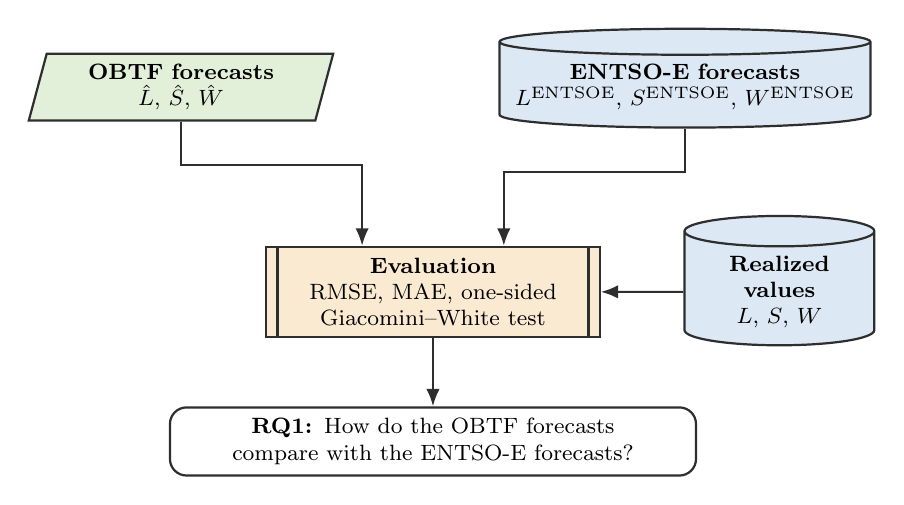
\begin{tikzpicture}[font=\footnotesize]

% ---- forecasts under comparison ----
\node[fgout=3.2cm] (own) at (-3.2, 0)
  {\textbf{OBTF forecasts}\\\(\hat{L}\), \(\hat{S}\), \(\hat{W}\)};
\node[fgdata=4.5cm, aspect=0.07] (ent) at (3.2, 0)
  {\textbf{\mbox{ENTSO-E} forecasts}\\\mbox{\(L^{\mathrm{ENTSOE}}\), \(S^{\mathrm{ENTSOE}}\), \(W^{\mathrm{ENTSOE}}\)}};

% ---- evaluation row ----
\node[fgeval=3.6cm] (eval) at (0,-2.6)
  {\textbf{Evaluation}\\RMSE, MAE, one-sided\\Giacomini--White test};
\node[fgdata=2.2cm] (real) at (4.4,-2.6)
  {\textbf{Realized values}\\\(L\), \(S\), \(W\)};

\node[fgrq=6.4cm] (rq) at (0,-4.5)
  {\textbf{RQ1:} How do the OBTF forecasts compare with the
   \mbox{ENTSO-E} forecasts?};

% ---- flows ----
\draw[fgflow] (own.south) -- ++(0,-0.55) -| ([xshift=-0.9cm]eval.north);
\draw[fgflow] (ent.south) -- ++(0,-0.55) -| ([xshift=0.9cm]eval.north);
\draw[fgflow] (real.west) -- (eval.east);
\draw[fgflow] (eval.south) -- (rq.north);

\end{tikzpicture}
\caption[OBTF forecast comparison for RQ1.]
{Design of RQ1. The OBTF load, solar, and wind
forecasts and the \mbox{ENTSO-E} forecasts are each scored against the realized
values on a matched panel. The OBTF forecasts use only information
available before the 12:00 deadline. Notation as in
Figure~\ref{fig:system_overview}.}
\label{fig:rq1_component_forecast_design}
\end{figure}


\FloatBarrier

\subsubsection{RQ2: Explicit Load and Renewable-Generation Forecasts in Price Forecasting}
\label{sec:rq2_price_experiments}

\hyperlink{rq:price_impact_generated_forecasts}{RQ2} is addressed by testing
how an explicit representation of load and renewable-generation forecasts
affects the price forecast. This is implemented by adding
\(\hat{L}_{d,q|d-1}\),
\(\hat{G}^{\mathrm{ren}}_{d,q|d-1}\), and
\(\widehat{RL}_{d,q|d-1}\) to the price model. The main
comparison is between \(\hat{P}^{\mathrm{base}}_{d,q|d-1}\) and
\(\hat{P}^{\mathrm{gen}}_{d,q|d-1}\). Both forecasts are produced with the same
boosted-tree model class, the same forecast creation time, the same evaluation
window, and the same price-lag, calendar, and raw weather inputs.
They differ only in whether \(\hat{L}_{d,q|d-1}\),
\(\hat{G}^{\mathrm{ren}}_{d,q|d-1}\), and
\(\widehat{RL}_{d,q|d-1}\) are included.
Since OBTF forecasts are produced by the separate OBTF load, solar, and wind models with task-specific weather representations, this comparison measures
the effect of the explicit load and renewable-generation forecast
representation rather than the effect of an identical raw weather information
set.

A secondary comparison uses the weather-free variant
\(\hat{P}^{\mathrm{gen},-\mathrm{wea}}_{d,q|d-1}\), which keeps OBTF forecasts but omits the raw weather features. Because OBTF forecasts
are derived from weather, comparing
\(\hat{P}^{\mathrm{gen},-\mathrm{wea}}_{d,q|d-1}\) with
\(\hat{P}^{\mathrm{base}}_{d,q|d-1}\) tests whether they can stand in for the raw
weather features, while comparing it with
\(\hat{P}^{\mathrm{gen}}_{d,q|d-1}\) shows whether the raw weather features
still add information beyond OBTF forecasts.

The previous-day and previous-week naive price forecasts are included in this
price forecast comparison. They are not used as benchmarks for the load, solar,
and wind forecasts because RQ1 concerns the quality of
OBTF forecasts relative to the corresponding \mbox{ENTSO-E}
day-ahead forecasts. In RQ2, their role is to show whether the price
models add value beyond simple price persistence.
Figure~\ref{fig:rq3_price_experiments_design} illustrates the RQ2 comparison
together with the weather-free variant and the naive benchmarks.

\begin{figure}[htbp]
\centering
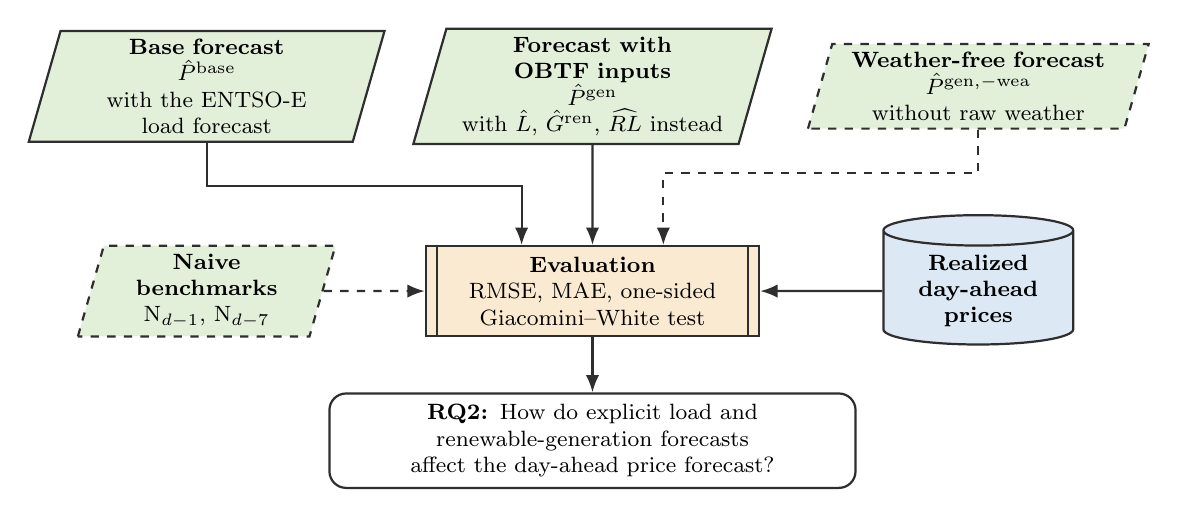
\begin{tikzpicture}[font=\footnotesize]

% ---- price forecast variants ----
\node[fgout=3.5cm] (base) at (-4.9, 0)
  {\textbf{Base forecast}\\\(\hat{P}^{\mathrm{base}}\)\\with the \mbox{ENTSO-E} load forecast};
\node[fgout=3.5cm] (gen) at (0, 0)
  {\textbf{Forecast with OBTF inputs}\\\(\hat{P}^{\mathrm{gen}}\)\\with \(\hat{L}\), \(\hat{G}^{\mathrm{ren}}\), \(\widehat{RL}\) instead};
\node[fgout=3.5cm, fgvar] (wea) at (4.9, 0)
  {\textbf{Weather-free forecast}\\\(\hat{P}^{\mathrm{gen},-\mathrm{wea}}\)\\without raw weather};

% ---- evaluation row ----
\node[fgout=2.4cm, fgvar] (naive) at (-4.9,-2.6)
  {\textbf{Naive benchmarks}\\\(\mathrm{N}_{d-1}\), \(\mathrm{N}_{d-7}\)};
\node[fgeval=3.6cm] (eval) at (0,-2.6)
  {\textbf{Evaluation}\\RMSE, MAE, one-sided\\Giacomini--White test};
\node[fgdata=2.2cm] (real) at (4.9,-2.6)
  {\textbf{Realized}\\\textbf{day-ahead prices}};

\node[fgrq=6.4cm] (rq) at (0,-4.5)
  {\textbf{RQ2:} How do explicit load and renewable-generation forecasts
   affect the day-ahead price forecast?};

% ---- flows ----
\draw[fgflow] (base.south) -- ++(0,-0.55) -| ([xshift=-0.9cm]eval.north);
\draw[fgflow] (gen.south) -- (eval.north);
\draw[fgaux]  (wea.south) -- ++(0,-0.55) -| ([xshift=0.9cm]eval.north);
\draw[fgaux]  (naive.east) -- (eval.west);
\draw[fgflow] (real.west) -- (eval.east);
\draw[fgflow] (eval.south) -- (rq.north);

\end{tikzpicture}
\caption[Price forecast comparison for RQ2.]
{Design of RQ2. The base forecast uses price history, calendar
features, weather, and the \mbox{ENTSO-E} load forecast, while
\(\hat{P}^{\mathrm{gen}}\) replaces the latter with the OBTF load,
renewable-generation, and residual-load forecasts. A weather-free variant and two
naive forecasts serve as secondary comparisons. Notation as in
Figure~\ref{fig:system_overview}.}
\label{fig:rq3_price_experiments_design}
\end{figure}


\FloatBarrier

\subsubsection{RQ3: Richer Information Sets over Time}
\label{sec:cutoff_sensitivity}

\hyperlink{rq:cutoff_sensitivity}{RQ3} is addressed through a
timing experiment that evaluates how electricity price forecast
performance changes with richer information sets over time. The
forecasting pipeline is rerun at the cutoff times
\(\mathcal{T}^{\mathrm{cut}}\) from Section~\ref{sec:operational_information_set}.
At each cutoff, the OBTF load, solar, and wind models of RQ1 and RQ2 are rerun
unchanged with only the inputs available before that time on day \(d-1\), so the OBTF forecasts entering the price model are themselves
cutoff-specific. Realized load and generation enter only up to the last
quarter-hour published at the start of the model run, allowing for a
publication delay of up to one hour \cite{euRegulation543_2013}. All cutoffs use the \mbox{ICON-D2} 06~UTC run, which is
complete about 80~minutes after its start and is therefore admissible from the
10:00 cutoff onward in both winter and summer time. Operationally, the earlier
cutoffs would use an earlier run (Table~\ref{tab:cutoff_accrual}). In the backtest this is not
possible, because the later 09~UTC run is complete only after 12:00 in summer
and the earlier 00 and 03~UTC runs were not archived for the first months of
the test period, so the
earlier cutoffs also use the 06~UTC run (Section~\ref{sec:limitations}). Because
all cutoffs share this weather run, moving
later in the morning can improve the forecasts through more recent realized load
and generation values, reserve-market auction results, and additional inputs
with later publication times. For load, this also
changes the admissible model setup: early cutoffs rely on the direct OBTF load model, while cutoffs after publication of the public
\mbox{ENTSO-E} load forecast can use the forecast-correction mode from
Section~\ref{sec:load_model}. Reserve-market results enter in stages as the
corresponding product auctions become observable: FCR
from 09:00, aFRR from 10:00, and mFRR from 11:00. The EXAA day-ahead price, published around 11:15,
becomes admissible only at the 12:00 cutoff and is included
there as a late price signal.
Table~\ref{tab:cutoff_accrual} lists the admissible inputs at each cutoff. Figure~\ref{fig:cutoff_sensitivity_design} illustrates
the timing experiment.

\begin{figure}[htbp]
\centering
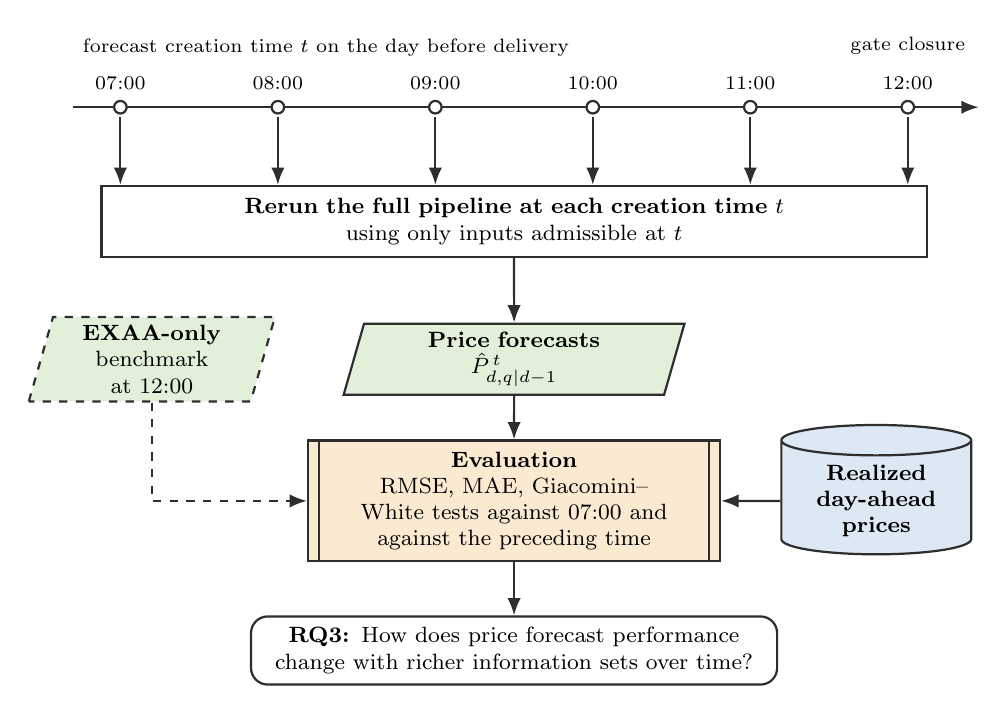
\begin{tikzpicture}[font=\footnotesize]

% ---- time axis of forecast creation times ----
\draw[thick, draw=fgLine, -{Latex[length=2.2mm,width=1.7mm]}] (-5.6,0) -- (5.9,0);
\foreach \x/\l in {-5/07:00, -3/08:00, -1/09:00, 1/10:00, 3/11:00, 5/12:00} {
  \draw[thick, draw=fgLine] (\x,0.08) -- (\x,-0.08);
  \node[font=\scriptsize, above] at (\x,0.1) {\l};
  \node[circle, draw=fgLine, thick, fill=white, inner sep=1.6pt] at (\x,0) {};
}
\node[font=\scriptsize, anchor=west] at (-5.6,0.75)
  {forecast creation time \(t\) on the day before delivery};
\node[font=\scriptsize, anchor=south] at (5,0.55) {gate closure};

% ---- rerun of the pipeline ----
\node[fgproc=10.2cm] (run) at (0,-1.45)
  {\textbf{Rerun the full pipeline at each creation time \(t\)}\\using only inputs admissible at \(t\)};
\foreach \x in {-5,-3,-1,1,3,5}
  \draw[fgflow] (\x,-0.12) -- (\x,0 |- run.north);

% ---- forecasts ----
\node[fgout=3.6cm] (fc) at (0,-3.2)
  {\textbf{Price forecasts}\\\(\hat{P}^{\,t}_{d,q|d-1}\)};
\node[fgout=2.3cm, fgvar] (exaa) at (-4.6,-3.2)
  {\textbf{EXAA-only}\\benchmark at 12:00};

% ---- evaluation ----
\node[fgeval=4.6cm] (eval) at (0,-5.0)
  {\textbf{Evaluation}\\RMSE, MAE, Giacomini--White tests
   against 07:00 and against the preceding time};
\node[fgdata=2.2cm] (real) at (4.6,-5.0)
  {\textbf{Realized}\\\textbf{day-ahead prices}};

\node[fgrq=6.4cm] (rq) at (0,-6.9)
  {\textbf{RQ3:} How does price forecast performance change with richer
   information sets over time?};

% ---- flows ----
\draw[fgflow] (run.south) -- (fc.north);
\draw[fgflow] (fc.south) -- (eval.north);
\draw[fgaux]  (exaa.south) |- (eval.west);
\draw[fgflow] (real.west) -- (eval.east);
\draw[fgflow] (eval.south) -- (rq.north);

\end{tikzpicture}
\caption[Information-set timing experiment for RQ3.]
{Design of RQ3. The full pipeline is rerun at six forecast
creation times from 07:00 to the 12:00 gate closure, each time with only the
information admissible at that time, and the resulting price forecasts are
compared with each other and with a compact EXAA-only benchmark. Notation as in
Figure~\ref{fig:system_overview}.}
\label{fig:cutoff_sensitivity_design}
\end{figure}


\FloatBarrier

\begin{table}[H]
  \centering
  \footnotesize
  \setlength{\tabcolsep}{5pt}
  \caption[Admissible inputs at each forecast creation time.]
  {Admissible inputs at each forecast creation time on day \(d-1\). A dash denotes an input that is not yet admissible.
  \textsuperscript{a}Due to data limitations, the backtest uses the 06~UTC run at
  every cutoff (Section~\ref{sec:limitations}).}
  \label{tab:cutoff_accrual}
  \begin{tabular}{@{}llllllc@{}}
    \toprule
    & \multicolumn{2}{l}{Weather run} & Realized & OBTF & Reserve & \\
    \cmidrule(lr){2-3}
    Cutoff & Operation & Backtest\textsuperscript{a} & data to & load model & products & EXAA \\
    \midrule
    07:00 & 03~UTC & 06~UTC & 05:30 & Direct & \(-\) & \(-\) \\
    08:00 & 03~UTC & 06~UTC & 06:30 & Direct & \(-\) & \(-\) \\
    09:00 & 03~UTC & 06~UTC & 07:30 & Direct & FCR & \(-\) \\
    10:00 & 06~UTC & 06~UTC & 08:30 & Direct & FCR, aFRR & \(-\) \\
    11:00 & 06~UTC & 06~UTC & 09:30 & Correction & FCR, aFRR, mFRR & \(-\) \\
    12:00 & 06~UTC & 06~UTC & 10:30 & Correction & FCR, aFRR, mFRR
      & \(\checkmark\) \\
    \bottomrule
  \end{tabular}
\end{table}

\FloatBarrier

\subsection{Evaluation Framework}
\label{sec:evaluation}

\subsubsection{Evaluation Panel and Error Metrics}
\label{sec:error_metrics}

The evaluation framework is shared across all RQs. Each
comparison uses
out-of-sample forecasts generated under the admissible information set for the
corresponding forecast creation time, over the test period from
1~February~2026 to 31~July~2026 defined in
Section~\ref{sec:experimental_design}. Models within the same RQ
are evaluated on the same delivery days and MTUs. If a model is
missing a forecast for a timestamp in the matched panel, the timestamp is
removed for all models in that specific comparison and the number of
observations is reported.

Let \(e^{m}_{d,q} = Y_{d,q} - \hat{Y}^{\,m}_{d,q|d-1}\) denote the forecast
error of model \(m\), and let \(\mathcal{E}\) be the matched evaluation panel.
All point models are estimated by minimizing squared error, so their forecasts
target the conditional mean of the delivery-period outcome. The primary metric
is therefore the root mean squared error (RMSE),
\[
  \operatorname{RMSE}(m)
  =
  \sqrt{\frac{1}{|\mathcal{E}|}
  \sum_{(d,q)\in\mathcal{E}}
  \bigl(e^{m}_{d,q}\bigr)^{2}},
\]
which rewards accurate estimation of that conditional mean and is the scoring
metric of the Energy-Arena submissions \cite{kleinebrahm2026energyarena}. The
mean absolute error (MAE)
\(\operatorname{MAE}(m) = |\mathcal{E}|^{-1} \sum_{(d,q)\in\mathcal{E}}
|e^{m}_{d,q}|\) is reported alongside it for every comparison, because it is a
standard accuracy metric in the electricity price forecasting literature and,
being expressed in the target unit, aids interpretation and comparison with
published work \cite{lago2021forecasting,hyndman2006another}. Price metrics are
reported in EUR/MWh. Load, solar, and wind
metrics are reported in MW.

\subsubsection{Paired Model Comparisons}
\label{sec:paired_model_comparisons}

Model comparisons are reported as relative RMSE changes. For a reference
forecast \(a\) and a challenger \(b\),
\[
  \Delta\operatorname{RMSE}_{a,b}
  =
  \frac{\operatorname{RMSE}(b) - \operatorname{RMSE}(a)}{\operatorname{RMSE}(a)},
\]
so a negative value means that \(b\) has a lower error than \(a\). When
statistical significance is assessed, the thesis uses the Giacomini-White (GW)
conditional predictive ability test \cite{giacomini2006tests} on the
squared-error loss, consistent with the squared-error training objective and the
RMSE metric. Because the 96 quarter-hourly prices of a delivery day are
forecast jointly, the test is applied to the daily mean loss differential
\(\bar{\delta}_{d}\) across the 96 MTUs. The test uses two instruments,
namely a constant and the previous day's differential \(\bar{\delta}_{d-1}\), so
the test statistic is asymptotically \(\chi^{2}\)-distributed with two degrees of
freedom. The test is
used one-sided, in the direction of the forecast with the lower average loss. The test provides supporting evidence, while the
main interpretation is based on the size, direction, and consistency of the
out-of-sample error differences. When several tests address the same question,
the chance that at least one of them appears significant by coincidence grows
with their number. Within each such family, namely each column of the RQ3 cutoff
results and the three pre-EXAA cutoffs of the reserve ablation, the p-values are
therefore additionally checked with the Holm procedure \cite{holm1979simple}. It
orders the \(m\) p-values of a family from smallest to largest, compares the
smallest with \(5\%/m\), the next with \(5\%/(m-1)\), and so on, and stops at
the first one that exceeds its threshold. This keeps the probability of any
false significant result within the family at 5\%.

\subsubsection{Feature Importance}
\label{sec:feature_importance}

As a diagnostic, the boosted-tree price model is analyzed with SHapley Additive exPlanations (SHAP) values
\cite{lundberg2017shap,lundberg2020treeshap}. SHAP values attribute each individual prediction to
its input features and are aggregated by summation within the feature groups
that make up the price model: price lags, calendar and holiday variables,
weather variables, the EXAA price and reserve-market auction results where
admissible, and the OBTF forecasts
\(\hat{L}_{d,q|d-1}\), \(\hat{G}^{\mathrm{ren}}_{d,q|d-1}\), and
\(\widehat{RL}_{d,q|d-1}\). Because SHAP values are signed, they also show the
direction of each feature's effect, that is, whether it raises or lowers the
forecast, which summary plots across all predictions make visible
\cite{lundberg2017shap,lundberg2020treeshap}, as in
Figure~\ref{fig:rq2_shap_beeswarm}. This analysis helps interpret whether the OBTF forecasts are actually
used by the price model.

\clearpage
\section{Results}
\label{sec:results}

\subsection{RQ1: OBTF Forecasts versus \mbox{ENTSO-E} Forecasts}
\label{sec:results_rq1}

Table~\ref{tab:rq1_component_forecast_results} compares OBTF
forecasts with the corresponding \mbox{ENTSO-E} day-ahead forecasts, each
evaluated against the same realized value. For load, the OBTF forecast is
the forecast-correction model of Section~\ref{sec:load_model}, created at the
final pre-gate-closure run before 12:00, so the comparison is against the
uncorrected \mbox{ENTSO-E} load forecast that this model takes as its baseline. The direct OBTF load model, which
uses no \mbox{ENTSO-E} forecast, is not part of the fixed comparison in
Table~\ref{tab:rq1_component_forecast_results}, but is benchmarked against
\mbox{ENTSO-E} separately below and enters RQ3 at cutoff times before the public
\mbox{ENTSO-E} load forecast is available. For solar and wind, the
\mbox{ENTSO-E} benchmark forecast is missing for a small number of timestamps,
which are dropped from the matched panel.

\begin{table}[htbp]
  \centering
  \small
  \setlength{\tabcolsep}{4.2pt}
  \caption[Accuracy of the OBTF load, solar, and wind forecasts versus \mbox{ENTSO-E}.]
  {Accuracy of OBTF load, solar, and wind forecasts compared with
  \mbox{ENTSO-E} forecasts.}
  \label{tab:rq1_component_forecast_results}
  \begin{threeparttable}
  \begin{tabular}{@{}lrrrrrrr@{}}
    \toprule
    Target & \(n\) & \multicolumn{2}{c}{RMSE} &
    \(\Delta\) RMSE\tnote{a} & \multicolumn{2}{c}{MAE} &
    \(p_{\mathrm{GW}}\)\tnote{b} \\
    \cmidrule(lr){3-4} \cmidrule(l){6-7}
    & & OBTF & \mbox{ENTSO-E} & & OBTF & \mbox{ENTSO-E}
    \\
    \midrule
    Load & 17,376 & \textbf{1,727} & 2,697 & \textbf{-36.0\%}
      & \textbf{1,350} & 2,140 & \(<0.001\) \\
    Solar gen. & 17,280 & 2,301 & \textbf{1,370} & +68.0\%
      & 1,109 & \textbf{747} & \(<0.001\) \\
    Wind gen. & 17,184 & 3,119 & \textbf{2,248} & +38.8\%
      & 2,092 & \textbf{1,450} & \(<0.001\) \\
    \bottomrule
  \end{tabular}
  \begin{tablenotes}[flushleft]
    \footnotesize
    \item[a] \(\Delta\) RMSE is computed relative to the corresponding
    \mbox{ENTSO-E} forecast. Negative values indicate lower errors of the OBTF forecast. All error values are in MW. The column \(n\) gives the
    number of matched observations used for the comparison. The evaluation
    window is 1~February~2026 to 31~July~2026. The renewable-generation
    comparisons have fewer observations because the \mbox{ENTSO-E} solar and
    wind benchmark forecasts are missing for some timestamps, and the wind
    comparison excludes 7~February~2026, for which no \mbox{ICON-D2} run with
    wind fields is archived.
    \item[b] One-sided GW p-value for the forecast with the lower
    RMSE against the alternative forecast, using paired squared-error loss
    differences.
  \end{tablenotes}
  \end{threeparttable}
\end{table}

The load result supports the first part of
\hyperlink{hyp:component_forecast_quality}{H1}. The OBTF load forecast
reduces the RMSE from 2,697~MW to 1,727~MW, a 36.0\%
error reduction relative to the \mbox{ENTSO-E} load forecast, with a comparable
reduction in MAE. This pattern is
consistent with the model design, because the OBTF load forecast used here corrects the public \mbox{ENTSO-E} forecast instead
of replacing it with an independent direct forecast. It can therefore combine
the public forecast with recent morning load and weather information available
before gate closure. Because the two forecasts do not share an information
cutoff, this is an operational rather than a like-for-like modeling comparison:
the \mbox{ENTSO-E} forecast is produced by an undisclosed model and issued at a
generally earlier, unspecified time, so the 36.0\% reduction measures the
operational value of the additional pre-gate-closure information the correction
exploits rather than a difference in modeling skill alone. A stricter comparison
nonetheless isolates a genuine modeling component: the direct OBTF load model, which
uses only open data and does not use the \mbox{ENTSO-E} forecast at all, still
reduces RMSE by 17.3\% relative to \mbox{ENTSO-E} when it is formed at the 10:30
cutoff at which the public forecast is published, a difference that is
statistically significant (GW p-value of 0.003). Correcting the
public forecast then extends this advantage to 36.0\%. Within this
operational setting, the OBTF load forecast is not only
competitive with the \mbox{ENTSO-E} forecast, but substantially more accurate in this
test window. The GW test supports this ranking with a p-value
below 0.001.

The renewable-generation comparison shows the opposite pattern. The OBTF solar forecast
has an RMSE of 2,301~MW compared with 1,370~MW for the \mbox{ENTSO-E} solar
forecast. The OBTF wind forecast has an RMSE of 3,119~MW compared with
2,248~MW for the \mbox{ENTSO-E} wind forecast. The \mbox{ENTSO-E}
renewable-generation forecasts therefore outperform the OBTF solar and
wind forecasts in this benchmark comparison. The GW test also
supports the \mbox{ENTSO-E} ranking for both renewable-generation targets. For
solar and wind, however, the \mbox{ENTSO-E} forecasts are not admissible inputs
for the operational price forecast studied in this thesis. The \mbox{ENTSO-E}
forecasts used here are not publicly observable before the 12:00
day-ahead gate closure, while the OBTF solar and wind forecasts are restricted
to information that is available before gate closure. The higher errors of the OBTF solar and wind
forecasts therefore do not rule out their relevance for the price model.

Overall, \hyperlink{hyp:component_forecast_quality}{H1} is supported. The
OBTF load forecast is not only competitive with but more accurate than
the \mbox{ENTSO-E} forecast, and the OBTF solar and wind forecasts have
higher errors than the \mbox{ENTSO-E} benchmarks, as expected. The renewable gap
is substantial, however, with an RMSE that is 68.0\% higher for solar and 38.8\%
higher for wind. The
result therefore establishes the empirical trade-off for RQ2: the OBTF solar and wind forecasts are less accurate than their
\mbox{ENTSO-E} benchmarks, but they are admissible inputs for the
price forecast. Whether this operationally available
representation still improves the price forecast is tested in RQ2.

\subsection{RQ2: Explicit Load and Renewable-Generation Forecasts in Price Forecasting}
\label{sec:results_rq2}

\hyperlink{rq:price_impact_generated_forecasts}{RQ2} tests how an explicit
representation of load and renewable-generation forecasts affects the
day-ahead price forecast.
This representation consists of the OBTF load forecast, the
OBTF combined renewable-generation forecast, and the OBTF
residual-load forecast.
Table~\ref{tab:rq2_price_results} reports the
out-of-sample accuracy of the two naive benchmarks and the three price
forecasts from the boosted-tree price model, all evaluated on the same matched panel of delivery days and
MTUs.

\begin{table}[htbp]
  \centering
  \small
  \setlength{\tabcolsep}{5.5pt}
  \caption[Price forecast accuracy with and without OBTF forecasts.]
  {Out-of-sample price forecast accuracy of the naive benchmarks and the
  price forecasts with and without OBTF load and renewable-generation forecasts.}
  \label{tab:rq2_price_results}
  \begin{threeparttable}
  \begin{tabular}{@{}lrrrrr@{}}
    \toprule
    Forecast & \(n\) & RMSE & \(\Delta\)RMSE\tnote{a} & MAE
      & \(p_{\mathrm{GW}}\)\tnote{b} \\
    \midrule
    \(\mathrm{N}_{d-1}\)
      & 17,184 & 49.69 & +40.0\% & 30.63 & \(<0.001\) \\
    \(\mathrm{N}_{d-7}\)
      & 17,184 & 60.31 & +69.9\% & 38.18 & \(<0.001\) \\
    \(\hat{P}^{\mathrm{base}}\)
      & 17,184 & 35.50 & --- & 20.82 & --- \\
    \(\hat{P}^{\mathrm{gen}}\)
      & 17,184 & \textbf{31.54} & \textbf{-11.2\%} & \textbf{18.05} & \(<0.001\) \\
    \(\hat{P}^{\mathrm{gen},-\mathrm{wea}}\)
      & 17,184 & 31.79 & -10.5\% & 18.18 & \(<0.001\) \\
    \bottomrule
  \end{tabular}
  \begin{tablenotes}[flushleft]
    \footnotesize
    \item[a] \(\Delta\)RMSE is computed relative to
    \(\hat{P}^{\mathrm{base}}\). Negative values indicate lower errors
    than the base price forecast. All error values are in EUR/MWh. The column
    \(n\) gives the number of matched observations. The evaluation window is
    1~February~2026 to 31~July~2026, with 7~February~2026 (no archived wind
    input) and 19~June~2026 (weather input unavailable) removed.
    \item[b] One-sided GW p-value between the row forecast and
    \(\hat{P}^{\mathrm{base}}\), for the forecast with the lower RMSE of
    the two, using paired squared-error loss differences.
  \end{tablenotes}
  \end{threeparttable}
\end{table}

Explicitly representing load and renewable generation improves the price
forecast. The price forecast with OBTF load and renewable-generation forecasts,
\(\hat{P}^{\mathrm{gen}}\), reduces the RMSE from
35.50~EUR/MWh for the base forecast
\(\hat{P}^{\mathrm{base}}\) to 31.54~EUR/MWh, a
reduction of 11.2\%, with a comparable reduction in MAE. The
GW test rejects equal predictive accuracy in favor of
\(\hat{P}^{\mathrm{gen}}\), with a p-value below 0.001.
\hyperlink{hyp:price_impact_generated_forecasts}{H2} is therefore supported: the explicit load and
renewable-generation forecast representation carries information that
\(\hat{P}^{\mathrm{base}}\) does not already recover from price lags, calendar
variables, raw weather, and the \mbox{ENTSO-E} load forecast.

The weather-free variant \(\hat{P}^{\mathrm{gen},-\mathrm{wea}}\) isolates where
this information comes from. It keeps the OBTF forecasts
but drops the raw weather features. Its RMSE of 31.79~EUR/MWh is statistically
indistinguishable from \(\hat{P}^{\mathrm{gen}}\), with a
GW p-value of 0.20, and it still improves on \(\hat{P}^{\mathrm{base}}\)
by essentially the same margin, with a p-value below 0.001. The raw weather features
therefore add no measurable accuracy once OBTF forecasts are included.
Because the OBTF load, solar, and wind forecasts are themselves derived
from weather, this is consistent with them carrying the price-relevant part of
the weather information available to the model.

Both naive benchmarks are far less accurate than the model-based forecasts. The
previous-day benchmark \(\mathrm{N}_{d-1}\) has an RMSE of 49.69~EUR/MWh and the
previous-week benchmark \(\mathrm{N}_{d-7}\) an RMSE of 60.31~EUR/MWh, against
35.50~EUR/MWh for \(\hat{P}^{\mathrm{base}}\) and 31.54~EUR/MWh for
\(\hat{P}^{\mathrm{gen}}\). All three model-based price forecasts
(\(\hat{P}^{\mathrm{base}}\), \(\hat{P}^{\mathrm{gen}}\), and
\(\hat{P}^{\mathrm{gen},-\mathrm{wea}}\)) outperform both benchmarks with
GW p-values below 0.001, and \(\mathrm{N}_{d-1}\) in turn
outperforms \(\mathrm{N}_{d-7}\). The model-based price forecasts therefore add
substantial value beyond simple price persistence.

Taken together with RQ1, this resolves the trade-off identified there. The OBTF solar and wind forecasts are less accurate than the \mbox{ENTSO-E}
benchmarks, but those benchmarks are not publicly
observable before gate closure and are not admissible for the price forecast. The OBTF
forecasts, which are available before gate closure, still let
\(\hat{P}^{\mathrm{gen}}\) improve significantly on \(\hat{P}^{\mathrm{base}}\),
which already uses price lags, calendar variables, raw weather, and the
\mbox{ENTSO-E} load forecast.

\subsection{RQ3: Richer Information Sets over Time}
\label{sec:results_rq3}

\hyperlink{rq:cutoff_sensitivity}{RQ3} evaluates how the operational
day-ahead price forecast changes as the information set expands during the
morning of day \(d-1\). All models predict the \mbox{DE-LU} day-ahead price at
quarter-hourly resolution and are evaluated on the same test period as RQ2. The cutoff-specific OBTF load, solar, and wind forecasts are generated
separately for each forecast creation time, so that the price model receives
only information that would have been available at the corresponding cutoff.
The 07:00, 08:00, 09:00, and 10:00 specifications use the direct OBTF
load forecast, while the 11:00 and 12:00 specifications use the correction of
the public \mbox{ENTSO-E} day-ahead load forecast. Reserve-market
features enter only after the assumed publication cutoff of the corresponding
product: FCR from 09:00, FCR and aFRR from 10:00, and FCR, aFRR, and mFRR from
11:00 onward. EXAA prices enter only at the 12:00 cutoff.

Table~\ref{tab:rq3_cutoff_results} and Figure~\ref{fig:rq3_cutoff_accuracy}
report the cutoff-grid results. Forecast accuracy improves over the morning, but
gradually and without a statistically significant step before 12:00. The 07:00
model reaches an RMSE of 32.63~EUR/MWh. The 08:00 and 09:00 models are close to
it, at 32.83 and 32.39~EUR/MWh. Neither improves significantly on the 07:00
baseline, with GW p-values of 1.00 and 0.42, and neither improves
significantly on the cutoff one hour earlier.

From 10:00 onward the error declines more clearly. The 10:00 model, which adds
the aFRR results to the FCR results, reaches an RMSE of 31.78~EUR/MWh. The 11:00
model, which additionally includes the mFRR results and switches to the load
correction mode, reaches 30.81~EUR/MWh, 5.6\% below the 07:00 baseline. Neither
gain is statistically significant, however. Against the 07:00 baseline the
p-values are 0.083 and 0.054, and none of the steps between consecutive cutoffs
before 12:00 is significant. The direction of the 11:00 reduction is consistent
with RQ1. Once the public \mbox{ENTSO-E} load forecast is published around
10:30, the OBTF load model switches from its direct forecast to the more
accurate correction mode. A reserve-market ablation
(Appendix~\ref{app:reserve_ablation}) shows that the reserve-market results lower
the error at every cutoff before 12:00, most at 10:00 with 3.4\%. None of these
reductions is significant after the Holm correction.

The largest improvement occurs once EXAA prices become available. The full
12:00 model, which combines residual load, OBTF renewable-generation forecasts,
weather, all reserve products, and EXAA prices, reaches an RMSE of
27.58~EUR/MWh, 10.5\% below the 11:00 forecast. This is the only step that
significantly improves on its preceding cutoff, and it also significantly
improves on the 07:00 baseline (\(p<0.001\)), in both cases also after the Holm
correction. The compact EXAA-only benchmark is slightly more accurate, with an
RMSE of 27.13~EUR/MWh. This indicates that EXAA prices contain a very strong late-market
signal, consistent with \textcite{ziel2015exaa}, who documents the predictive
value of the earlier-closing EXAA auction for the German day-ahead market. In
the current specification, adding the full set of fundamental and reserve
features on top of EXAA does not improve the 12:00 point forecast. The
EXAA-only model is statistically indistinguishable from the full 12:00
specification, with a GW p-value of 0.65. This matches
\textcite{eiser2026operational}, who likewise found the compact EXAA-only model
to be the best-performing specification for this market.

\begin{table}[htbp]
  \centering
  \small
  \setlength{\tabcolsep}{5pt}
  \caption[Price forecast accuracy at each morning cutoff.]
  {Selected cutoff-grid price forecast results for RQ3.}
  \label{tab:rq3_cutoff_results}
  \begin{threeparttable}
  \begin{tabular}{@{}lrrrrr@{}}
    \toprule
    Forecast specification & RMSE & MAE & \(n\)
      & \(p_{\mathrm{GW}}^{07}\)\tnote{a} & \(p_{\mathrm{GW}}^{\mathrm{prev}}\)\tnote{b} \\
    \midrule
    07:00 & 32.63 & 18.34 & 17,184 & --- & --- \\
    08:00 & 32.83 & 18.31 & 17,184 & 1.00 & 1.00 \\
    09:00 & 32.39 & 18.25 & 17,184 & 0.42 & 0.43 \\
    10:00 & 31.78 & 17.81 & 17,184 & 0.083 & 0.091 \\
    11:00 & 30.81 & 17.53 & 17,184 & 0.054 & 0.14 \\
    12:00 & 27.58 & 13.72 & 17,184 & \(<0.001\) & \(<0.001\) \\
    12:00, EXAA-only & \textbf{27.13} & \textbf{13.62} & 17,184 & \(<0.001\) & 0.65 \\
    \bottomrule
  \end{tabular}
  \begin{tablenotes}[flushleft]
    \footnotesize
    \item[a] One-sided GW p-value, squared-error loss, against the
    07:00 forecast.
    \item[b] One-sided GW p-value, squared-error loss, against the
    preceding row. For the EXAA-only model, this is the full 12:00 specification.
    \item Errors in EUR/MWh.
  \end{tablenotes}
  \end{threeparttable}
\end{table}

\begin{figure}[htbp]
  \centering
  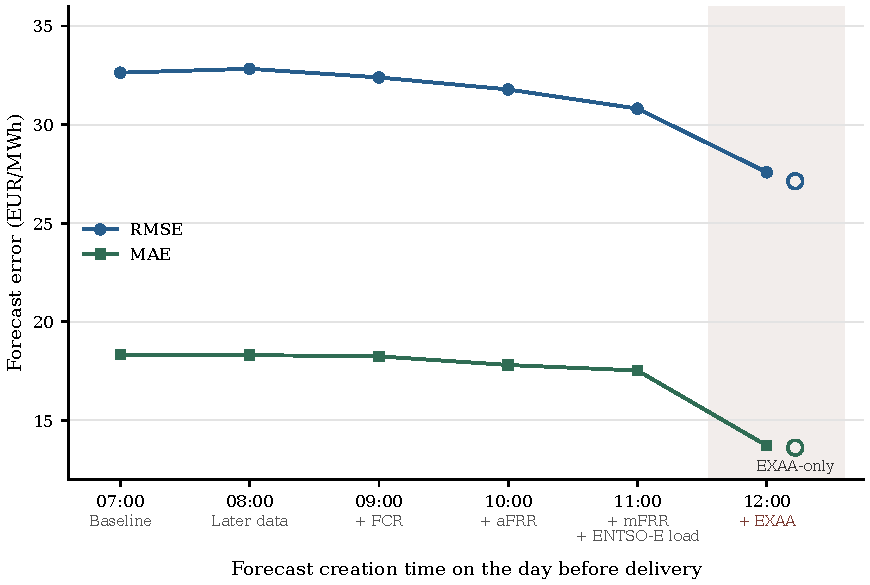
\includegraphics[width=0.78\textwidth]{figures/rq3_cutoff_accuracy.pdf}
  \caption[Price forecast accuracy across forecast creation times.]
  {Price forecast accuracy across the forecast creation times of the cutoff
  grid. The labels below each time name the information added at that cutoff,
  and realized data advance by one hour at every step. The shaded area marks the
  12:00 cutoff, at which EXAA prices become admissible. The hollow markers show
  the compact EXAA-only benchmark.}
  \label{fig:rq3_cutoff_accuracy}
\end{figure}

\FloatBarrier

\hyperlink{hyp:cutoff_sensitivity}{H3} is therefore only partly supported.
Later and richer information sets lower the price forecast error, and the RMSE
at 11:00 is 5.6\% below the 07:00 baseline, but before the EXAA price becomes
available none of these gains is statistically significant. The only significant
improvement, also after the Holm correction, is the step to 12:00. At that
cutoff the EXAA price captures most of the information relevant for the point
forecast, so the compact EXAA-only model matches the full specification, a known
effect for this market rather than a contribution of this thesis.

\FloatBarrier

\subsection{Diagnostic Feature Importance}
\label{sec:results_feature_importance}

The boosted-tree price forecasts are also analyzed with the SHAP values
introduced in Section~\ref{sec:feature_importance}. The forecast experiment
refits a separate LightGBM model for each delivery day on its rolling training
window. For this diagnostic, and for each selected specification, these daily
models are refitted for every delivery day in the evaluation window with the same
training window and hyperparameters, and their SHAP contributions are computed
for all MTUs with LightGBM's built-in TreeSHAP decomposition, then
aggregated by the feature groups defined in Section~\ref{sec:feature_importance}.
Because the price model is fitted on the variance-stabilized target of
Section~\ref{sec:price_model}, the contributions live in that transformed space
and are interpretable in direction and relative magnitude rather than as EUR/MWh
amounts. The grouped shares reported here are unit-free ratios of each group's
contribution to the total, so they are comparable across models but describe
relative importance in the transformed space, not EUR/MWh contributions. They
are diagnostic relative importances within the fitted model, not causal effects.

Figure~\ref{fig:rq2_feature_importance} reports the grouped contribution shares
for the RQ2 price models. In the base model, raw weather and price lags account
for most of the contribution mass, with shares of 43.1\% and 35.4\%, respectively,
and the \mbox{ENTSO-E} load forecast contributes 21.4\%. Once OBTF
forecasts are added, the structure of the model changes: the OBTF
residual-load forecast becomes the most important group, with a contribution
share of 42.3\% against 24.7\% for price lags, while raw weather falls to
13.0\% and the OBTF renewable-generation forecast contributes 15.3\%. In the
weather-free variant, residual load and renewable generation absorb the
weather-driven information directly, at 45.4\% and 21.7\%. This supports the interpretation from RQ2
that the OBTF load and renewable-generation forecasts provide a compact
weather-informed representation of the power-system state.

\begin{figure}[htbp]
  \centering
  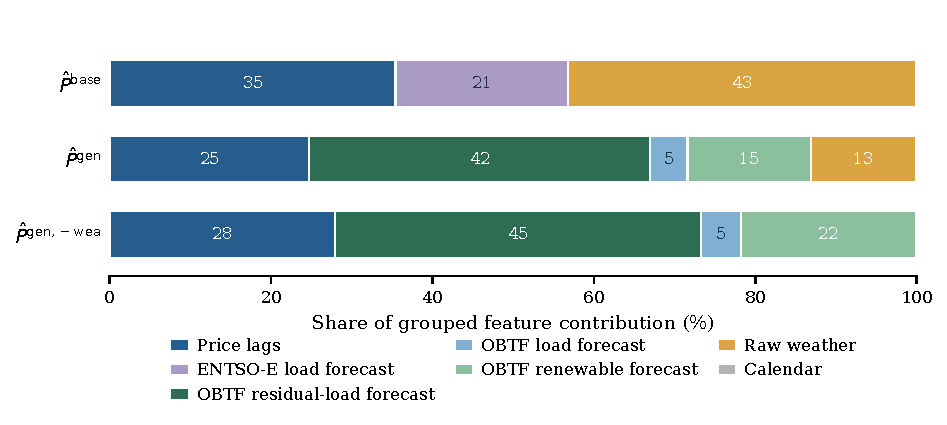
\includegraphics[width=0.86\textwidth]{figures/rq2_feature_importance_bars.pdf}
  \caption[Feature-importance shares for the RQ2 price models.]
  {Grouped feature-contribution shares for the RQ2 price models, as percentages
  of the mean absolute grouped SHAP contribution. The diagnostic covers all delivery days and MTUs in the evaluation window. Shares may not sum exactly to 100 because of
  rounding.}
  \label{fig:rq2_feature_importance}
\end{figure}

Figure~\ref{fig:rq3_feature_importance} reports the same diagnostic for selected
cutoff-grid models. Before EXAA prices become available, the residual-load
forecast and the price lags drive the price forecasts, alongside the renewable-generation
forecast, raw weather, and a growing reserve-market block. The reserve-market
share rises once aFRR information is available, from 4.4\% at 09:00 to 18.5\% at
10:00, and to 20.3\% at 11:00 as mFRR is added. The fitted models therefore make
substantial use of the reserve-market results, even though their contribution to
accuracy is not robustly significant (Section~\ref{sec:results_rq3}). At 12:00,
EXAA prices dominate the feature contributions, at 66.9\% of the mass, although
all other feature blocks are available. Together with the statistically
indistinguishable accuracy of the full 12:00 model and the EXAA-only model, this
is consistent with the late EXAA signal already containing most of the
short-horizon price information that the other feature blocks provide.
Appendix~\ref{app:feature_details} reports the leading subgroups for
\(\hat{P}^{\mathrm{gen}}\) and the 12:00 model, and shows the direction of the
leading effects.

\begin{figure}[htbp]
  \centering
  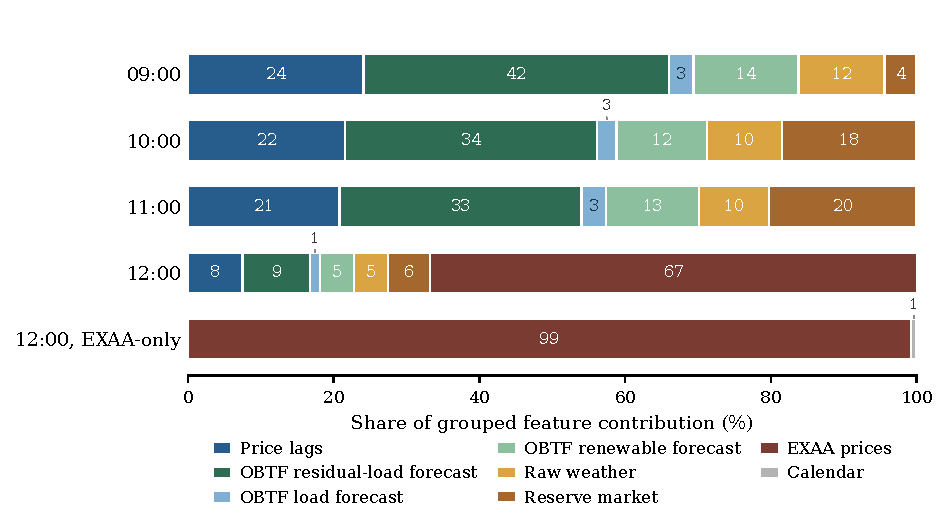
\includegraphics[width=0.86\textwidth]{figures/rq3_feature_importance_bars.pdf}
  \caption[Feature-importance shares for selected RQ3 cutoff models.]
  {Grouped feature-contribution shares for selected RQ3 cutoff models, as
  percentages of the mean absolute grouped SHAP contribution. The calendar group
  is below 1\% throughout. The
  diagnostic covers all delivery days and MTUs in the evaluation
  window. Shares may not sum exactly to 100 because
  of rounding.}
  \label{fig:rq3_feature_importance}
\end{figure}

\clearpage
\section{Discussion}
\label{sec:discussion}

\subsection{Do OBTF Load and Renewable Forecasts Improve Price Forecasts?}
\label{sec:discussion_rq2}

The OBTF forecasts improve the price forecast. Replacing the
published \mbox{ENTSO-E} load forecast with the OBTF load, combined
renewable-generation, and residual-load forecasts lowers the day-ahead price
RMSE by 11.2\% relative to the base price forecast, and the improvement is
statistically significant. Both forecasts use the same estimator, the same
forecast creation time, and the same price-lag, calendar, and raw-weather
inputs. They do not, however, share the same information set. The OBTF models
draw on a much richer weather representation, installed capacity from the
MaStR, population weights, and realized load, which the base
model does not receive directly, because hundreds of such features could not be
estimated from 70 daily training observations. The gain therefore measures the
value of this information delivered in the compact form of explicit forecasts,
not the value of the forecast representation alone
(Section~\ref{sec:limitations}).
The OBTF load and renewable-generation forecasts thus carry
predictive information that the price model does not recover on its own from
price history, raw weather, and the public load forecast.
This agrees with \textcite{maciejowska2021enhancing}, who show that including
load, wind, and solar forecasts, and improving their accuracy, yields more
accurate day-ahead price forecasts. Their comparison is against price models
without these forecasts, whereas the base forecast here already contains raw
weather, so the result extends their finding to a price model that already has
access to the underlying weather information.

The weather-free variant refines this interpretation. A price model that keeps
the OBTF forecasts but drops the raw weather features is statistically
indistinguishable from the model that retains both, and it still improves on the
base forecast by essentially the same margin. Once the OBTF forecasts
are included, the two-cluster raw weather features thus add no detectable
accuracy. This is consistent with how the forecasts are constructed, because
each is produced by a task-specific model that already distills the relevant
weather signal into an expected load, solar, or wind quantity. For the
data-limited price model, these few summary variables appear to be a more usable
form of the weather information than the raw weather from which they are
derived, although a non-significant difference does not prove that the raw
weather is redundant.

The most operationally relevant finding emerges when this result is read together
with RQ1. The OBTF solar and wind forecasts are less accurate than the
corresponding \mbox{ENTSO-E} benchmarks, yet they still improve the price
forecast, whereas the more accurate \mbox{ENTSO-E} renewable-generation forecasts,
which several price studies use as direct inputs
\cite{trebbien2023probabilistic,marcjasz2023distributional,hilger2024multivariate},
cannot be used at all because they are published only after gate closure. For
an operational price forecast, accuracy and admissibility are therefore both
required. A more accurate benchmark that is not observable before the deadline
cannot serve as an input, and an admissible forecast is useful only if it adds
information beyond price history, weather, and the public load forecast. The
OBTF forecasts satisfy both conditions, and the OBTF load forecast additionally exceeds the accuracy of the public forecast it is compared to.

\subsection{Operational Value of Waiting}

RQ3 shows that the accuracy of the operational price forecast improves as the
morning progresses and the admissible information set grows, but gradually and,
before 12:00, without statistically significant steps. Between 07:00 and 09:00
the forecast barely changes. From 10:00, when the aFRR results become available, and 11:00, when the public load
forecast and the mFRR results enter, the error
declines more clearly and is 5.6\% lower at 11:00 than at 07:00. On the
six-month test period, however, these gains are not statistically significant,
which may partly reflect that the backtest uses the same weather run at all
cutoffs (Section~\ref{sec:limitations}). A
participant who must commit early therefore loses little by forecasting at 07:00
rather than waiting until 11:00, although the direction of the evidence favors
waiting.

A further and larger gain comes at the gate-closure cutoff, once the EXAA price
is admissible. The EXAA auction clears earlier than the SDAC auction and its
price is a direct market estimate of the same day-ahead quantity, so it is
unsurprising that it carries more short-horizon information than any fundamental
input, consistent with the predictive value of the EXAA auction documented by
\textcite{ziel2015exaa}. That a compact model using the EXAA price alone matches
the full specification is a known property of this market rather than a finding
of this thesis \cite{eiser2026operational}, and the feature-importance analysis
reflects it, with the EXAA price accounting for about two-thirds of the
contribution mass at 12:00.

This does not diminish the value of the OBTF forecasts but clarifies
where each source matters. The EXAA price is published only shortly before gate
closure, so throughout the earlier part of the morning, while a participant is
still forming a bid rather than submitting it at the deadline, no market price is
yet available. Across those cutoffs the forecast rests on price lags, weather, the OBTF load and renewable-generation forecasts, and the reserve-market results,
which lower the error at every cutoff before 12:00, although not by a robustly
significant margin. Once the EXAA price arrives, it dominates.

\subsection{Role of Weather and Public Inputs}

The literature review left open how weather is best represented in a day-ahead
price model. The weather-free variant and the feature-importance results help
answer this question. In the base model,
raw weather is one of the two largest groups of inputs, so the fitted model
relies heavily on weather. When the OBTF
forecasts are added, the importance of raw weather drops sharply and is taken over by the OBTF residual-load and renewable-generation forecasts, and the
weather-free variant shows that the raw weather features can be removed
altogether without a measurable loss. For this data-limited price model, the
OBTF forecasts are therefore at least as useful a representation of
the weather-driven system state as the two-cluster raw weather fields, plausibly
because they condense a much richer weather signal into a small number of
variables that are already aligned with how weather affects prices. The dominance of the OBTF residual-load forecast is consistent with residual demand as a
central driver of the price \cite{do2021residualDemand,pape2016fundamentals} and
with the explainable machine-learning analysis of \textcite{trebbien2023merit},
who find load, wind, and solar generation to be the most important features for
German day-ahead prices. This
contrasts with operational pipelines that instead feed spatially resolved
weather directly into the price model in place of the unavailable renewable-generation forecasts \cite{eiser2026operational}, and with studies that select among a large
set of weather variables within the price model \cite{ludwig2015bigdata}. Meteorological
forecasts have been shown to improve German price forecasts beyond the day-ahead
horizon \cite{sgarlato2023weatherPredictions}. At the day-ahead horizon, the
results here suggest that explicitly
forecasting load and renewable generation is a promising way to bring weather
information into a day-ahead price model, subject to the caveat on the unequal
weather information discussed in the limitations.

The public data sources play distinct and complementary roles. The published
\mbox{ENTSO-E} load forecast is a useful baseline whose accuracy the
OBTF load model improves on by correcting it with later information, so
in this setting the public forecast is more useful as a starting point for
correction than as a final input. The reserve-market results add some information about system tightness
before any market price is available, although their effect is not robust on
this test period. The EXAA price is the single most informative
public input at gate closure, but it is admissible only at the very end of the
morning. Read together, these inputs form a sequence in which fundamental and
reserve information dominate early and the exchange price dominates late, and an
operational price model benefits from using each of them at the point in the
morning where it becomes available.

\subsection{Openness and Operational Deployment}

A defining property of the pipeline is that it is fully open and operationally
admissible. Every input is drawn from open, automatically retrievable sources,
namely open weather forecasts, the \mbox{ENTSO-E} Transparency Platform, the
MaStR, and gridded population data, so the self-generated load,
solar, wind, and price forecasts can be generated and extended without
proprietary inputs. The preprocessing, the OBTF models, and the price model
are released as a modular, configuration-driven codebase that is ready for
operational use and deployment, so each stage can be reused and extended.
Together with the daily Energy-Arena submission, this follows the call of
\textcite{lago2021forecasting} for open-access benchmarks in electricity price
forecasting. By replacing the
post-gate-closure \mbox{ENTSO-E} renewable-generation forecasts with
OBTF forecasts, the pipeline also respects the operational timing,
so the reported accuracy reflects what a participant could actually have
produced before the deadline.

The pipeline is additionally submitted to Energy-Arena \cite{kleinebrahm2026energyarena}, where its load, solar, wind,\footnote{The Energy-Arena
\mbox{DE-LU} wind challenge targets onshore wind generation, so only the onshore
component of the OBTF wind forecast is submitted there, whereas the OBTF wind forecast evaluated in this thesis is total wind generation, onshore and
offshore.} and price forecasts are
scored against realized outcomes under a common gate-closure deadline and shared
in the benchmark's cooperative mode so that other forecasters can reuse them, for
example as ensemble members. This provides a continuous, forward-looking, and
leakage-controlled evaluation that extends the fixed test period of this thesis
and lets the OBTF forecasts serve as a reusable building block for further
work.

Beyond serving the price model, the OBTF component forecasts are
directly reusable. Regenerated from the open repository, the OBTF load forecast improves on the public \mbox{ENTSO-E} load forecast and can be used in its place,
while the OBTF solar and wind forecasts provide admissible substitutes for the
\mbox{ENTSO-E} renewable-generation forecasts, which are not published before
gate closure. Unlike the \mbox{ENTSO-E} forecasts, which are produced by
undisclosed models and cannot be inspected, the OBTF forecasts are
fully transparent, because their inputs, models, and construction are open and
can be examined and adapted rather than taken as given.

\subsection{Limitations}
\label{sec:limitations}

The load benchmarking in RQ1 is an operational rather than a like-for-like
modeling comparison. The OBTF load forecast corrects the public
\mbox{ENTSO-E} forecast with information available up to the pre-gate-closure
cutoff, whereas the \mbox{ENTSO-E} forecast is produced by an undisclosed model
at a generally earlier, unspecified cutoff. A comparison that fixes both
forecasts to an identical cutoff is therefore not feasible, and the reported load
improvement should be read as the operational value of correcting the public
forecast before gate closure rather than as evidence of a superior standalone
load model. This caveat concerns only the interpretation of the standalone load
comparison. Because the OBTF load forecast serves solely as an admissible input to the
price model, its only operational requirement is to be available before the 12:00
gate closure, so producing it at a later cutoff than the \mbox{ENTSO-E} forecast,
with correspondingly more recent information, is by design rather than a
disadvantage.

The central caveat of the RQ2 comparison, discussed in
Section~\ref{sec:discussion_rq2}, is that the base price model and the OBTF models do
not share the same information set. The base model receives raw weather only
through a compact two-cluster aggregation of the \mbox{ICON-D2} fields and none
of the capacity, population, and realized-load inputs of the OBTF models. A
comparison that supplied the base model with all of these inputs directly would
isolate the effect of the explicit representation, but hundreds of such features
cannot be estimated reliably from 70 daily training observations. The OBTF forecasts avoid this by splitting the
problem. Load, solar, and wind generation depend on different weather
variables, such as temperature for load, irradiance and cloud cover for solar,
and wind speed for wind. Without the first-stage forecasts, a single price model
would have to receive all of these variables at once. With them, each OBTF model uses only the weather it needs, and the price model receives the result as
a small number of forecast series, namely load, renewable generation, and
residual load. This limitation is thus at the same time the central appeal of
the approach.

The evaluation covers a single test window from February to July 2026, which is
the period for which post-transition quarter-hourly prices and the full set of
operational inputs are available. The results therefore describe one half-year of
a market that only recently moved to quarter-hourly clearing, and the autumn and
mid-winter months lie outside the test window. Whether the reported effects are
stable across seasons and across years with different fuel-price and
renewable-capacity conditions cannot be established from this sample, and a longer
multi-year evaluation would be needed to settle it. The ongoing Energy-Arena submission
extends this evidence with each new delivery day.

A major limitation of RQ3 concerns the weather input. The earlier
\mbox{ICON-D2} runs that would be admissible at the 07:00 to 09:00 cutoffs are
not archived for the whole test period, so all cutoffs use the 06~UTC run,
which is available only from about 09:20. The early cutoffs therefore receive a
more recent weather forecast than they could use in operation, which favors
them. At the same time, the backtest cannot capture any improvement from newer
weather runs over the morning, although weather is a central input of both the
OBTF and the price models. Both effects bias the measured gain from waiting
downward and may explain why the gains before 12:00 are not statistically
significant. A backtest with the operational run schedule of
Table~\ref{tab:cutoff_accrual}, possible once the earlier runs have been archived
over a full test period, would resolve this.

The OBTF solar and wind forecasts remain less accurate than the
\mbox{ENTSO-E} benchmarks, and the feature-importance analysis attributes more of
the price model's contribution to the OBTF load and residual-load forecasts than to the OBTF renewable-generation forecast (Section~\ref{sec:results_feature_importance}). The
OBTF solar and wind forecasts are thus admissible and useful but not competitive
in absolute accuracy, and closing this gap is a limitation of the current OBTF models rather than a property of the price model. The capacity data from the
current MaStR also include late-registered units that were not
yet known at the time, an effect the rolling bias correction partly absorbs. In
addition, the archived \mbox{ICON-D2} irradiance is incomplete or implausible on a
few days in June 2026. These days are retained, so the affected solar forecasts,
and through them the price forecasts, carry these input errors. As with the OBTF load forecast, however, the comparison is not on equal footing. The \mbox{ENTSO-E}
solar and wind benchmarks are produced by undisclosed models and, being published
only after gate closure, may draw on later weather runs and more recent
information than the OBTF forecasts, which are restricted to the
pre-gate-closure cutoff. Part of the observed gap may therefore reflect this
information and timing advantage rather than modeling skill alone, and how much of
it is genuinely attributable to the OBTF models cannot be established from
this comparison.

The feature-importance analysis is diagnostic rather than causal. The SHAP
contributions describe how the fitted model distributes its predictions across
inputs on the sampled data, not the true causal effect of each input, and they
are computed on the variance-stabilized model target so that only their direction
and relative magnitude are interpretable.

Finally, the thesis evaluates point forecasts only. Operational trading and risk
management typically require the full predictive distribution, and the pipeline
does not yet produce or evaluate probabilistic price forecasts.

\subsection{Future Work}

Several extensions follow directly from these limitations. The most immediate is
to close the accuracy gap of the OBTF solar and wind forecasts, for
example through multi-model weather ensembles \cite{bruninx2026windensembles}, wind speeds interpolated to the
turbine-specific hub heights recorded in the MaStR, or an
explicit treatment of curtailment, since more accurate renewable-generation forecasts would
strengthen the fundamental contribution to the price model.

The estimators themselves could also be revisited. Tabular
foundation models such as TabPFN are designed for small training sets
\cite{hollmann2025tabpfn}, which makes them a natural candidate for the
data-limited price model with its 70-day training window.

Beyond point forecasts, the pipeline could be extended to probabilistic
forecasting. The OBTF models could provide quantile forecasts of load, solar, and
wind generation as price-model inputs, which \textcite{uniejewski2026probabilistic}
show to lower the price RMSE by up to 13\% compared with point inputs for the
German market. The same OBTF forecasts and cutoff structure could feed a
distributional or quantile price model \cite{marcjasz2023distributional}, which would make the operational value of
the approach measurable in terms of the full predictive distribution rather than
the conditional mean alone.

Further gains may come from a broader admissible information set. Cross-border
prices and residual-load forecasts of neighboring bidding zones, as well as fuel
and emission-allowance prices, are known to carry predictive information for
German day-ahead prices
\cite{trebbien2023probabilistic,hilger2024multivariate,pape2016fundamentals},
and incorporating them within the open-data and
pre-gate-closure constraints of this thesis would show how much further the
operational forecast can be improved.

Finally, a longer and multi-seasonal evaluation would establish the stability of
the reported effects across market regimes, and extending the setup to the
intraday markets that follow the day-ahead auction would broaden its operational
relevance.

\clearpage
\section{Conclusion}
\label{sec:conclusion}

The main contribution of this thesis is a set of fully operational forecasting
models for load, solar, and wind generation based exclusively on open data, the
OBTF models. They are released as part of an open pipeline that enforces
forecast-time information availability and that others can rerun and reuse.
Their daily submission to the Energy-Arena benchmark
\cite{kleinebrahm2026energyarena} lets anyone verify their accuracy beyond
the test period of this thesis. In
contrast to the \mbox{ENTSO-E} forecasts, whose methods are not disclosed, their
inputs and construction are fully open. Each model is either more accurate than its
\mbox{ENTSO-E} counterpart, as for load, or admissible before gate closure when
the \mbox{ENTSO-E} forecast is not, as for solar and wind. Used as explicit
inputs, the OBTF forecasts improve the operational day-ahead price forecast for
the \mbox{DE-LU} bidding zone, in which every input must be available before the
12:00 gate closure. The models can therefore be reused as admissible,
transparent inputs in other operational applications.

For RQ1, the OBTF load forecast is more accurate than the published
\mbox{ENTSO-E} forecast in the operational setting, reducing the load RMSE by
36.0\%. The OBTF solar and wind forecasts are less accurate than the
\mbox{ENTSO-E} forecasts, but those benchmarks are not published before gate
closure and cannot be used in an operational price forecast.

For RQ2, adding the OBTF load, combined renewable-generation, and
residual-load forecasts to the price model lowers the day-ahead price RMSE by
11.2\%, a statistically significant improvement. The weather-free variant is
statistically indistinguishable in accuracy, so the raw weather fields add no detectable accuracy once these
forecasts are included, which makes them a compact representation of the
weather-driven system state for the price model.

For RQ3, price accuracy improves as the morning progresses, but gradually. Up to 11:00 the error falls by 5.6\% without a statistically significant step,
which may partly reflect that the backtest uses the same weather run at all
cutoffs. The only significant gain follows at gate closure once the EXAA price
becomes admissible. That
the earlier-clearing EXAA price captures most of the achievable accuracy at 12:00
is a known property of this market rather than a result of this thesis
\cite{eiser2026operational}. Before any market price is available, the forecast
rests on price lags, weather, the OBTF forecasts, and the
reserve-market results.

The findings are relevant beyond the market and period studied here. Day-ahead
prices depend strongly on weather-driven load and renewable generation
\cite{sensfuss2008meritOrder,pape2016fundamentals}, and the corresponding public
forecasts are either less accurate than the OBTF forecast or unavailable before
gate closure. Turning open weather data into admissible load and
renewable-generation forecasts is therefore valuable in other bidding zones with
the same gate-closure constraint. In a field where forecasts are often produced by
undisclosed models and evaluated retrospectively, such an open and continuously
benchmarked pipeline offers a transparent operational baseline that others can
reproduce, extend, and compare against. The thesis is thus a step toward
day-ahead price forecasting that is operational, open, and explicit about what
information it uses and when.

\clearpage
\clearpage
\appendix
\renewcommand{\thesubsection}{\thesection\arabic{subsection}}
\refstepcounter{section}
\section*{Appendix \thesection}
\markboth{Appendix \thesection}{Appendix \thesection}
\addcontentsline{toc}{section}{Appendix \thesection}
\label{app:additional_material}

% Number appendix floats with the appendix letter (Table A1, Figure A1, ...)
\renewcommand{\thetable}{\thesection\arabic{table}}
\renewcommand{\thefigure}{\thesection\arabic{figure}}
\setcounter{table}{0}
\setcounter{figure}{0}

\subsection{Data Availability and Operational Timing}
\label{app:data_timing}

Table~\ref{tab:data_timing} documents the main availability times shown in
Figure~\ref{fig:operational_timeline}. Regulatory deadlines and exchange rules
are binding latest times. Platform behavior and publication latencies describe
typical availability and can deviate on individual days. The admissible
information set of Section~\ref{sec:operational_information_set} is applied
with these availability times at every cutoff.

\begin{table}[H]
  \centering
  \footnotesize
  \caption[Data sources and availability times of the operational inputs.]
  {Sources and status of the operational availability times used in
  Figure~\ref{fig:operational_timeline}.}
  \label{tab:data_timing}
  \begin{tabular}{@{}>{\raggedright\arraybackslash}p{0.26\textwidth}
                  >{\raggedright\arraybackslash}p{0.34\textwidth}
                  >{\raggedright\arraybackslash}p{0.32\textwidth}@{}}
    \toprule
    Element & Operational timing used & Source and status \\
    \midrule
    SDAC gate closure
    & 12:00 on day \(d-1\)
    & Exchange rule \cite{epexSpotPowerMarket} \\
    \addlinespace
    \mbox{ENTSO-E} day-ahead load forecast
    & Regulatory deadline two hours before gate closure, observed available
      around 10:30 on day \(d-1\) in the data collection
    & Regulatory deadline, Regulation 543/2013 Art.~6(1)(b)
      \cite{euRegulation543_2013}, availability observed by the data
      collection \\
    \addlinespace
    \mbox{ENTSO-E} realized load
    & Published no later than one hour after the operating period
    & Regulatory deadline, Art.~6(1)(a) \cite{euRegulation543_2013} \\
    \addlinespace
    \mbox{ENTSO-E} realized wind and solar generation
    & Published no later than one hour after the operating period, with
      initial estimates updated as measured data becomes available
    & Regulatory deadline, Art.~16(1)(j) \cite{euRegulation543_2013} \\
    \addlinespace
    \mbox{ENTSO-E} day-ahead wind and solar forecast
    & Published after the 12:00 gate closure and no later than
      18:00 on day \(d-1\)
    & Publication time reported for the \mbox{ENTSO-E} Transparency Platform
      \cite{kleinebrahm2026energyarena}, with the publication requirement set
      under Art.~14(2)(d) \cite{euRegulation543_2013} \\
    \addlinespace
    EXAA day-ahead prices
    & Auction closes at 10:15 on day \(d-1\). EXAA
      day-ahead prices for Germany are published on the \mbox{ENTSO-E} Transparency
      Platform around 11:15
    & Exchange rule \cite{exaaTradingRules2025}, publication time
      \cite{entsoeTransparency,eiser2026operational} \\
    \addlinespace
    Control-reserve auction results
    & German control-reserve capacity auctions for delivery day \(d\) close on
      day \(d-1\) at 08:00 (FCR), 09:00 (aFRR), and 10:00 (mFRR). Their
      results are used from one hour after gate closure. A check on
      28~September~2026 found them published 14 to 23 minutes after gate
      closure
    & Auction platform \cite{regelleistungNet2026} \\
    \addlinespace
    SDAC auction results
    & Released after gate closure and therefore not admissible before
      12:00
    & Market-coupling process \cite{epexSpotMarketCoupling} \\
    \addlinespace
    \mbox{ICON-D2} weather forecasts
    & A new run starts every three hours and is complete about 80 minutes after
      its start
    & DWD Open Data \cite{dwdIconForecastData} and Open-Meteo documentation
      \cite{openMeteoForecastApi} \\
    \bottomrule
  \end{tabular}
\end{table}

\FloatBarrier

\subsection{Model Configurations}
\label{app:model_configs}

Table~\ref{tab:model_configs} summarizes the final configuration of every model
in the pipeline. All models use a rolling origin: for each delivery day they are
refitted on a trailing training window ending on the day before delivery. The
load, solar, and wind forecasting models use their own task-specific weather
representations and forecast creation times, while the price models use the
coarse two-cluster weather aggregation selected on the development period
(Appendix~\ref{app:price_base_selection}). The RQ3 cutoff models reuse the RQ2
price-model configuration and vary only the admissible information set with the
forecast creation time.

\begin{table}[H]
  \centering
  \footnotesize
  \setlength{\tabcolsep}{3.8pt}
  \caption[Final model configurations.]
  {Final configuration of each pipeline model. The window is the length of the
  rolling training window in days. All weather features are derived from the DWD
  ICON-D2 model, accessed through DWD Open Data or the Open-Meteo API.}
  \label{tab:model_configs}
  \begin{tabular}{@{}>{\raggedright\arraybackslash}p{0.135\textwidth}
                  >{\raggedright\arraybackslash}p{0.11\textwidth}
                  >{\raggedright\arraybackslash}p{0.055\textwidth}
                  >{\raggedright\arraybackslash}p{0.20\textwidth}
                  >{\raggedright\arraybackslash}p{0.27\textwidth}@{}}
    \toprule
    Model & Estimator & Win. & Weather representation & Key inputs \\
    \midrule
    Load, correction
      & LightGBM & 224 & \mbox{ICON-D2}, 25 clusters, population-weighted
      & \mbox{ENTSO-E} load forecast, realized load to 10:30, calendar, weather \\
    \addlinespace
    Load, direct
      & LightGBM & 224 & \mbox{ICON-D2}, 25 clusters, population-weighted
      & Realized load to the cutoff, calendar, and weather, without the
        \mbox{ENTSO-E} forecast \\
    \addlinespace
    Solar
      & Hist.\ gradient boosting & 90 & \mbox{ICON-D2}, 25 clusters per TSO,
        capacity-weighted
      & Clear-sky geometry and physics baseline, irradiance, cloud cover,
        installed capacity \\
    \addlinespace
    Wind
      & Hist.\ gradient boosting & 180 & ICON-D2 incl.\ hub-height fields, 100 clusters
        incl.\ offshore, capacity-weighted
      & Hub-height wind speed, power-curve and cubic transforms, installed
        capacity \\
    \addlinespace
    Price \(\hat{P}^{\mathrm{base}}\)
      & LightGBM, 300 trees & 70 & \mbox{ICON-D2}, 2 clusters
      & Price lags, calendar, weather, \mbox{ENTSO-E} load forecast \\
    \addlinespace
    Price \(\hat{P}^{\mathrm{gen}}\)
      & LightGBM, 300 trees & 70 & \mbox{ICON-D2}, 2 clusters
      & As \(\hat{P}^{\mathrm{base}}\), with the \mbox{ENTSO-E} load forecast
        replaced by the OBTF load, renewable-generation, and residual-load
        forecasts \\
    \addlinespace
    Price, RQ3 cutoffs
      & LightGBM, 300 trees & 70 & \mbox{ICON-D2}, 2 clusters, 06~UTC run
        at all cutoffs
      & Inputs admissible at each cutoff, adding reserve-market results from
        09:00 and EXAA prices at 12:00 \\
    \bottomrule
  \end{tabular}
\end{table}

\FloatBarrier

\subsection{Additional Price Forecast Results}
\label{app:price_results}

This appendix reports the development-period selection of the base price model,
which fixes the rolling training window and the weather-cluster count used
throughout the price experiments.

\subsubsection{Selection of the Base Price Model Window and Weather Clustering}
\label{app:price_base_selection}

The rolling training window and the raw-weather cluster count of the base
price model are selected by a staged search on the development period
(20~December~2025 to 31~January~2026), so that no design choice depends on the
test period. The search is a coordinate descent. The training window is chosen
first at a fixed mid-range count of sixteen weather clusters, the boosted-tree
hyperparameters are chosen next at the selected window, and the number of
weather clusters is chosen last at the selected window. The hyperparameter stage
selects a small tree size and moderate \(L_2\) regularization, with the number of
leaves having little effect at the available sample size and stronger
regularization degrading accuracy. The two knobs that carry the comparison are
therefore the window length and the cluster count, reported below.

Table~\ref{tab:price_base_window} varies the training window from 28 days to an
expanding window that uses all post-transition history. Development-period
accuracy improves up to 70 days and then plateaus, and the expanding window
gives no meaningful further gain. A 70-day window is selected.

\begin{table}[H]
  \centering
  \small
  \caption[Base price model training-window selection.]
  {Development-period accuracy of the base price model over the rolling
  training window, at sixteen weather clusters and 300 boosted-tree rounds. The
  expanding window uses all post-transition history. The selected window is in
  bold. Errors are in EUR/MWh.}
  \label{tab:price_base_window}
  \begin{tabular}{@{}lrr@{}}
    \toprule
    Training window (days) & RMSE & MAE \\
    \midrule
    28        & 26.75 & 16.79 \\
    42        & 26.37 & 16.36 \\
    56        & 24.49 & 14.75 \\
    \textbf{70} & \textbf{23.30} & \textbf{14.19} \\
    Expanding & 23.21 & 14.28 \\
    \bottomrule
  \end{tabular}
\end{table}

Table~\ref{tab:price_base_clusters} fixes the window at 70 days and varies the
number of weather clusters from 1 to 100. Accuracy is best at two clusters and
degrades as the spatial resolution increases, while the mean training time per
delivery day grows from about twelve seconds at one cluster to nearly half an
hour at one hundred clusters. Finer spatial resolution therefore raises the
training cost sharply without improving accuracy, so no accuracy--runtime
trade-off arises from using a coarse grid. The selected two-cluster
representation is the most accurate and among the cheapest, with only the
single-cluster grid marginally faster but less accurate. A plausible explanation
is that the data-limited price model, which sees at most 70 daily training rows,
cannot exploit fine spatial weather detail and instead overfits it. Two clusters
are selected. To keep the sweep tractable given this steep cost growth, the cluster
search uses 100 boosted-tree rounds rather than the 300 rounds of the final
model, which is why the same sixteen-cluster, 70-day configuration appears at a
lower error in Table~\ref{tab:price_base_window}, run at 300 rounds, than in
Table~\ref{tab:price_base_clusters}. The selection assumes that using fewer
rounds shifts the error level roughly uniformly rather than reordering the
cluster counts. This assumption is not tested for every count, but the selected
two-cluster configuration is retrained at the full 300 rounds for all reported
results.
Figure~\ref{fig:price_base_cluster_pareto} shows the same result as an
accuracy--runtime frontier. The selection is robust to the choice of metric. The two-cluster
representation minimizes both the RMSE and the MAE, and the 70-day window has
the lowest MAE of all windows while lying on the RMSE plateau.

\begin{table}[H]
  \centering
  \small
  \caption[Base price model weather-clustering selection.]
  {Development-period accuracy and mean training cost of the base price
  model over the number of weather clusters, at a 70-day window and 100
  boosted-tree rounds. Training time is the mean wall-clock time per delivery
  day of the rolling backtest. The selected cluster count is in bold. Errors are
  in EUR/MWh.}
  \label{tab:price_base_clusters}
  \begin{tabular}{@{}lrrr@{}}
    \toprule
    Weather clusters & RMSE & MAE & Training time (s/day) \\
    \midrule
    1   & 24.21 & 14.89 & 12 \\
    \textbf{2}   & \textbf{23.70} & \textbf{14.49} & 17 \\
    5   & 24.02 & 14.86 & 31 \\
    8   & 23.96 & 14.63 & 49 \\
    12  & 24.31 & 14.92 & 79 \\
    16  & 24.33 & 14.95 & 110 \\
    25  & 24.56 & 15.03 & 189 \\
    40  & 25.43 & 15.61 & 363 \\
    64  & 25.12 & 15.58 & 758 \\
    100 & 25.49 & 15.64 & 1712 \\
    \bottomrule
  \end{tabular}
\end{table}

\begin{figure}[htbp]
  \centering
  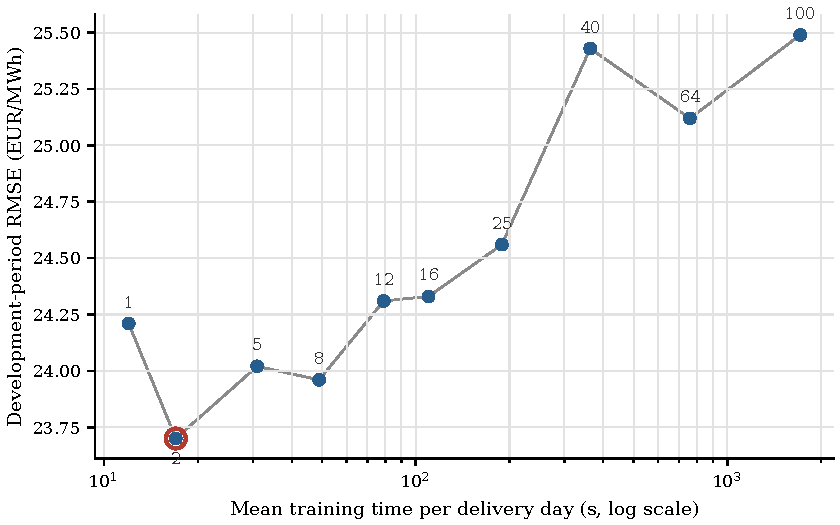
\includegraphics[width=0.72\textwidth]{figures/price_base_cluster_pareto.pdf}
  \caption[Accuracy--runtime frontier of the base price model weather
  clustering.]
  {Development-period RMSE against mean training time per delivery day for the
  base price model, over weather-cluster counts from 1 to 100 at a 70-day
  window. The selected two-cluster representation is highlighted.}
  \label{fig:price_base_cluster_pareto}
\end{figure}

\FloatBarrier

\subsubsection{Reserve-Market Ablation}
\label{app:reserve_ablation}

Table~\ref{tab:reserve_ablation} isolates the effect of the reserve-market
features by comparing each cutoff price model with an otherwise identical model
that excludes the reserve-market covariates, on the same matched panel. Before
the EXAA price is admissible, adding the reserve-market results lowers the RMSE
at every cutoff, by 1.1\% at 09:00, 3.4\% at 10:00, and 2.1\% at 11:00. Only the
10:00 improvement, after the aFRR results enter, is significant on its own, and
it does not remain significant after the Holm correction across the three
pre-EXAA cutoffs. At the 12:00 cutoff, once the EXAA price is admissible, the
reserve-market features no longer help and slightly increase the error, which is
consistent with the EXAA signal absorbing most of the short-horizon price
information. The reserve-market results therefore contribute to the gradual
improvement before 12:00, but their effect cannot be established robustly on
this test period.

\begin{table}[H]
  \centering
  \small
  \caption[Reserve-market ablation for the cutoff price models.]
  {Reserve-market ablation for the cutoff price models. Each row compares a
  cutoff model without reserve-market features against the otherwise identical
  model with them, on the matched test panel from 1~February~2026 to
  31~July~2026 (\(n=17{,}184\)). The \emph{With reserve} \mbox{RMSE} column holds
  the selected cutoff models and matches their RMSE in
  Table~\ref{tab:rq3_cutoff_results}, while the \emph{No reserve} column is the
  counterfactual without reserve-market features. Errors are in EUR/MWh.}
  \label{tab:reserve_ablation}
  \begin{threeparttable}
  \begin{tabular}{@{}llrrrr@{}}
    \toprule
    Cutoff & Reserve products & \multicolumn{2}{c}{RMSE}
      & \(\Delta\)RMSE & \(p_{\mathrm{GW}}\)\tnote{a} \\
    \cmidrule(lr){3-4}
    & & No reserve & With reserve & & \\
    \midrule
    09:00 & FCR & 32.76 & 32.39 & -1.1\% & 0.23 \\
    10:00 & FCR, aFRR & 32.89 & 31.78 & -3.4\% & 0.025 \\
    11:00 & FCR, aFRR, mFRR & 31.46 & 30.81 & -2.1\% & 0.11 \\
    12:00\tnote{b} & FCR, aFRR, mFRR & 27.27 & 27.58 & +1.1\% & --- \\
    \bottomrule
  \end{tabular}
  \begin{tablenotes}[flushleft]
    \footnotesize
    \item[a] One-sided GW p-value, squared-error loss, with against
    without reserve-market features. None remains significant after a Holm
    correction across the three pre-EXAA cutoffs.
    \item[b] Both 12:00 models include the EXAA price. The reserve-market features
    do not improve the forecast, so no p-value is reported.
  \end{tablenotes}
  \end{threeparttable}
\end{table}

\FloatBarrier

\subsubsection{Detailed Feature-Importance Results}
\label{app:feature_details}

The grouped shares in Section~\ref{sec:results_feature_importance} aggregate over
feature groups. A subgroup collects all the per-MTU columns of
one signal, such as the lagged price on day \(d-1\), which enters as a separate
feature for each of the 96 quarter-hours, or the OBTF residual-load forecast.
Tables~\ref{tab:rq2_top_features} and \ref{tab:rq3_top_features} break the feature
groups down one level finer, into these subgroups, for the price forecast with
OBTF load and renewable-generation forecasts \(\hat{P}^{\mathrm{gen}}\) and for the full 12:00 cutoff
model.

Shares use the same normalization as the grouped shares in
Figures~\ref{fig:rq2_feature_importance} and~\ref{fig:rq3_feature_importance}, so
a group with a single subgroup, such as the EXAA price, matches those figures
exactly. Subgroups within a group need not sum to the group share, because
importance is measured as a mean absolute contribution: when two subgroups in the
same group push the forecast in opposite directions on a given prediction, their
effects partly cancel in the group total, so the group's absolute contribution is
smaller than the sum of the subgroups' absolute contributions.

For \(\hat{P}^{\mathrm{gen}}\), the residual-load level is the single largest
subgroup, followed by the previous-day price lag, with the residual-load ramp,
wind, radiation, and the OBTF renewable-generation forecasts contributing further.
For the 12:00 model, the EXAA price subgroup alone accounts for about
two-thirds of the contribution mass, far ahead of the residual-load level, the
previous-day price lag, and the reserve-market results, which confirms the dominance of the late EXAA signal
at the final cutoff. Figure~\ref{fig:rq2_shap_beeswarm} shows the direction of the
leading effects in \(\hat{P}^{\mathrm{gen}}\). Higher recent prices and higher
residual load push the forecast up, while higher wind generation pushes it down,
in the economically expected direction.

\begin{table}[H]
  \centering
  \small
  \caption[Leading feature contributions in the RQ2 price model.]
  {Subgroups with the largest mean absolute SHAP contribution for \(\hat{P}^{\mathrm{gen}}\), combining each signal
  over its MTUs.
  Shares are percentages of the model's total grouped contribution.}
  \label{tab:rq2_top_features}
  \begin{tabular}{@{}llr@{}}
    \toprule
    Subgroup & Group & Share (\%) \\
    \midrule
    Residual load & Residual load & 36.9 \\
    Lagged price (day \(d-1\)) & Price lags & 21.2 \\
    Residual load ramp & Residual load & 9.9 \\
    Wind generation & Renewables & 9.9 \\
    Shortwave diffuse radiation & Raw weather & 6.2 \\
    Wind speed & Raw weather & 5.8 \\
    Shortwave direct radiation & Raw weather & 5.0 \\
    Load forecast & Load & 4.6 \\
    Solar generation & Renewables & 4.5 \\
    Total renewable generation & Renewables & 4.1 \\
    \bottomrule
  \end{tabular}
\end{table}

\begin{table}[H]
  \centering
  \small
  \caption[Leading feature contributions in the 12:00 cutoff model.]
  {Subgroups with the largest mean absolute SHAP contribution for the
  full 12:00 cutoff model, combining each signal over its MTUs.
  Shares are percentages of the model's total grouped contribution.}
  \label{tab:rq3_top_features}
  \begin{tabular}{@{}llr@{}}
    \toprule
    Subgroup & Group & Share (\%) \\
    \midrule
    EXAA price & EXAA & 66.9 \\
    Residual load & Residual load & 6.9 \\
    Lagged price (day \(d-1\)) & Price lags & 6.1 \\
    Reserve market & Reserve & 5.7 \\
    Residual load ramp & Residual load & 3.9 \\
    Wind generation & Renewables & 2.8 \\
    Wind speed & Raw weather & 2.7 \\
    Shortwave diffuse radiation & Raw weather & 1.9 \\
    Total renewable generation & Renewables & 1.7 \\
    Shortwave direct radiation & Raw weather & 1.6 \\
    \bottomrule
  \end{tabular}
\end{table}

\begin{figure}[H]
  \centering
  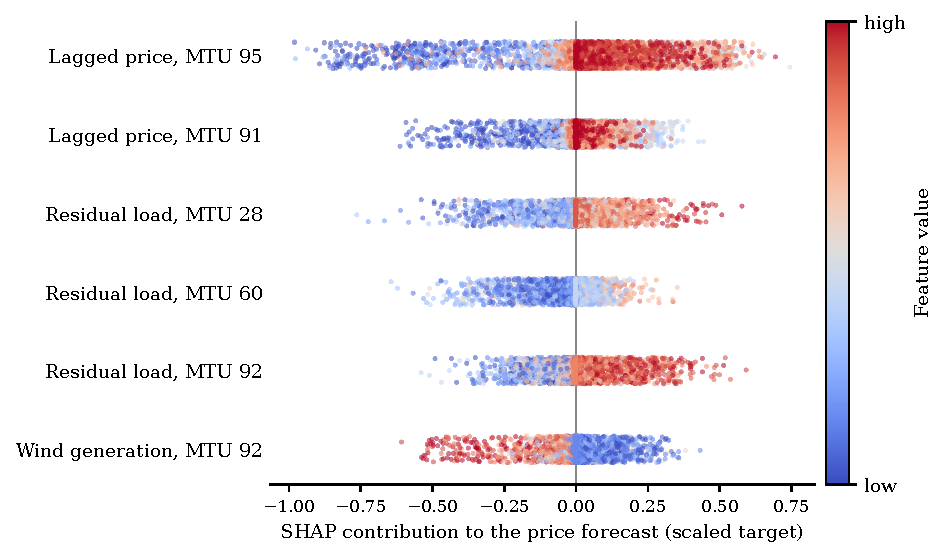
\includegraphics[width=0.82\textwidth]{figures/rq2_shap_beeswarm.pdf}
  \caption[Direction of the leading feature effects in the RQ2 price model.]
  {Direction of the leading feature effects for \(\hat{P}^{\mathrm{gen}}\). Each
  point is one sampled prediction, its horizontal position is the feature's SHAP
  contribution to that forecast, and its color is the feature value from low
  (blue) to high (red). Contributions are on the scaled model target, so only
  their direction and relative magnitude are interpretable.}
  \label{fig:rq2_shap_beeswarm}
\end{figure}

\FloatBarrier


%%%%%%%%%%%%%%%%%%%%%%%%%%%%%%%%%%%%%%%%%%%%%%%%%%%%%%%%%%%%%%%%%%%%%%%%%%%%%%%%
%% DATA AND CODE AVAILABILITY
%%%%%%%%%%%%%%%%%%%%%%%%%%%%%%%%%%%%%%%%%%%%%%%%%%%%%%%%%%%%%%%%%%%%%%%%%%%%%%%%

\clearpage
\thispagestyle{plain}
\markboth{}{}
\section*{Data and Code}
\addcontentsline{toc}{section}{Data and Code}

The operational forecasting pipeline developed in this thesis is publicly
available at

\begin{center}
\url{https://github.com/davideig/DA_Price_Forecasting_DE_LU_Fundamental}
\end{center}

\noindent It provides the data-access integrations and endpoints, the
preprocessing and modeling code, and the configuration files, so that open-data
load, solar, wind, and day-ahead price forecasts for the \mbox{DE-LU} market can be
generated and extended without building the data infrastructure from scratch.

\noindent The resulting load, solar, wind, and day-ahead price forecasts are also
submitted to Energy-Arena
\cite{kleinebrahm2026energyarena} under the username
\nolinkurl{Eiglsperger_2026}, using the benchmark's \enquote{open immediately} cooperative
mode, so that other forecasters can download them before the target period is
realized and reuse them, for example as members of forecast ensembles.

%%%%%%%%%%%%%%%%%%%%%%%%%%%%%%%%%%%%%%%%%%%%%%%%%%%%%%%%%%%%%%%%%%%%%%%%%%%%%%%%
%% REFERENCES
%%%%%%%%%%%%%%%%%%%%%%%%%%%%%%%%%%%%%%%%%%%%%%%%%%%%%%%%%%%%%%%%%%%%%%%%%%%%%%%%

\clearpage
\pagestyle{plain}
\printbibliography
\clearpage

%%%%%%%%%%%%%%%%%%%%%%%%%%%%%%%%%%%%%%%%%%%%%%%%%%%%%%%%%%%%%%%%%%%%%%%%%%%%%%%%
%% STATUTORY DECLARATION (Selbststaendigkeitserklaerung)
%%%%%%%%%%%%%%%%%%%%%%%%%%%%%%%%%%%%%%%%%%%%%%%%%%%%%%%%%%%%%%%%%%%%%%%%%%%%%%%%
\thispagestyle{empty}
\vspace*{4.0cm}

\noindent
\begin{sloppypar}
Ich versichere wahrheitsgem\"a\ss, die Arbeit selbstst\"andig verfasst, alle
benutzten Hilfsmittel vollst\"andig und genau angegeben und alles kenntlich
gemacht zu haben, was aus Arbeiten anderer unver\"andert oder mit
Ab\"anderungen entnommen wurde sowie die Satzung des KIT zur Sicherung guter
wissenschaftlicher Praxis in der jeweils g\"ultigen Fassung beachtet zu haben.
\end{sloppypar}

\vspace{2.0cm}

\noindent
\begin{minipage}[t]{0.45\textwidth}
Karlsruhe, den 30.09.2026
\end{minipage}
\hfill
\begin{minipage}[t]{0.35\textwidth}
\hrule
\vspace{0.3cm}
David Maximilian Eiglsperger
\end{minipage}

\clearpage

%%%%%%%%%%%%%%%%%%%%%%%%%%%%%%%%%%%%%%%%%%%%%%%%%%%%%%%%%%%%%%%%%%%%%%%%%%%%%%%%
%% ANLAGE: DECLARATION ON THE USE OF GENERATIVE AI (official KIT form)
%%%%%%%%%%%%%%%%%%%%%%%%%%%%%%%%%%%%%%%%%%%%%%%%%%%%%%%%%%%%%%%%%%%%%%%%%%%%%%%%
\pagestyle{empty}

\noindent{\large\bfseries Anlage: Erkl\"arung zur Verwendung generativer
KI-Systeme\par}

\vspace{0.8cm}

\noindent Bei der Erstellung der Arbeit habe ich die folgenden auf
k\"unstlicher Intelligenz (KI) basierten Systeme benutzt:

\vspace{0.4cm}
\noindent
\begin{tabular}{@{}ll@{}}
1. & Claude (Anthropic) \\
2. & Claude Code (Anthropic) \\
3. & Codex (OpenAI) \\
\end{tabular}

\vspace{0.6cm}

\noindent Ich erkl\"are weiterhin, dass ich

\vspace{0.3cm}
\noindent
\begin{tabular}{@{}p{1.4em}p{0.90\textwidth}@{}}
$\boxtimes$ & mich aktiv \"uber die Leistungsf\"ahigkeit und Beschr\"ankungen der
oben genannten KI-Systeme informiert habe, \\[0.4em]
$\boxtimes$ & \"uberpr\"uft habe, dass die mithilfe der oben genannten KI-Systeme
generierten und von mir \"ubernommenen Inhalte faktisch richtig sind, \\[0.4em]
$\boxtimes$ & mir bewusst bin, dass ich als Autor dieser Arbeit die Verantwortung
f\"ur die in ihr gemachten Angaben und Aussagen trage. \\
\end{tabular}

\vspace{0.6cm}

\noindent Die oben genannten KI-Systeme habe ich wie im Folgenden dargestellt
eingesetzt.

\vspace{0.3cm}

\begin{longtable}{@{}>{\raggedright\arraybackslash}p{0.24\textwidth}
                    >{\raggedright\arraybackslash}p{0.19\textwidth}
                    >{\raggedright\arraybackslash}p{0.49\textwidth}@{}}
\toprule
\textbf{Arbeitsschritt} & \textbf{Eingesetzte(s) KI-System(e)} &
\textbf{Beschreibung der Verwendungsweise} \\
\midrule
\endfirsthead
\toprule
\textbf{Arbeitsschritt} & \textbf{Eingesetzte(s) KI-System(e)} &
\textbf{Beschreibung der Verwendungsweise} \\
\midrule
\endhead
\bottomrule
\endlastfoot
Generierung von Ideen und Konzeption der Arbeit & Claude &
Diskussion m\"oglicher Forschungsfragen und experimenteller Designs als
Ausgangspunkt f\"ur eigene Entscheidungen \\
\addlinespace
Literatursuche & -- & -- \\
\addlinespace
Literaturanalyse & Claude & Unterst\"utzung beim Verst\"andnis spezifischer
Methoden und Modelle \\
\addlinespace
Literaturverwaltung und Zitationsmanagement & Claude &
\"Uberpr\"ufung von Referenzeintr\"agen auf formale Vollst\"andigkeit. Alle
Zitate wurden selbstst\"andig auf Korrektheit gepr\"uft \\
\addlinespace
Auswahl von Methoden und Modellen & Claude, Claude Code &
Diskussion geeigneter Prognosemethoden und Modellspezifikationen. Die finale
Methodenauswahl wurde selbst getroffen \\
\addlinespace
Datensammlung und -analyse & Claude, Claude Code, Codex &
Unterst\"utzung beim Verst\"andnis der ICON-D2-, \mbox{ENTSO-E}- und weiteren
Open-Data-Strukturen. \"Uberpr\"ufung der Datenverarbeitungspipeline in Python \\
\addlinespace
Generierung von Programmcodes & Claude Code, Codex &
Implementierung und \"Uberarbeitung der Skripte und Konfigurationen im
Repository. Korrektur von LaTeX-Code. Fehlersuche und Optimierung bestehender
Code-Abschnitte \\
\addlinespace
Erstellung von Visualisierungen & Claude, Claude Code &
Unterst\"utzung bei Implementierung und Verbesserung von Abbildungen in Python
und LaTeX \\
\addlinespace
Interpretation und Validierung & Claude &
Diskussion von Modellergebnissen als Denkansatz. Die finale Interpretation und
Validierung erfolgten selbstst\"andig \\
\addlinespace
Strukturierung des Texts der Arbeit & Claude &
Vorschl\"age f\"ur Gliederung und Kapitelaufbau \\
\addlinespace
Formulierung des Texts der Arbeit & Claude &
Erste Formulierungsideen und Umformulierung von W\"ortern und Abs\"atzen \\
\addlinespace
\"Ubersetzung des Texts der Arbeit & -- & -- \\
\addlinespace
Redigieren des Texts & Claude &
Rechtschreib-, Grammatik- und Stilpr\"ufung sowie Konsistenzpr\"ufung. Alle
Korrekturen wurden selbstst\"andig gepr\"uft und eigenverantwortlich
\"ubernommen \\
\addlinespace
Vorbereitung der Pr\"asentation des Texts & -- & -- \\
\addlinespace
Sonstiges & -- & -- \\
\end{longtable}

\vspace{1.0cm}

\noindent
\begin{minipage}[t]{0.45\textwidth}
Karlsruhe, den 30.09.2026
\end{minipage}
\hfill
\begin{minipage}[t]{0.35\textwidth}
\hrule
\vspace{0.3cm}
David Maximilian Eiglsperger
\end{minipage}

\clearpage

\end{document}
